%\documentclass[12pt]{article}
\documentclass[12pt]{report} % for chapters
%\usepackage{fullpage}
%\usepackage[top=1in,bottom=1in,left=1in,right=1in]{geometry}
\usepackage[margin=1in, paperwidth=8.5in, paperheight=11in]{geometry}
\usepackage[english]{babel}
\usepackage[utf8x]{inputenc}
\usepackage{amsmath}
\usepackage{graphicx}
\usepackage{caption}
\usepackage[depth=subsection]{bookmark}
\usepackage{multirow}
\usepackage[usestackEOL]{stackengine}
%https://www.sharelatex.com/learn/Code_listing
%For code view in latex

\usepackage{pdflscape}

\usepackage{listings}


%\usepackage[linktocpage=true]{hyperref}
\hypersetup{
    pdfborder = {0 0 0}
}

\usepackage[colorinlistoftodos]{todonotes}
\usepackage{chngcntr}
\usepackage{url}
%header and footer package
\usepackage{fancyhdr}
\usepackage[en-US]{datetime2}

%clearing default page heading and footer
\pagestyle{fancy}



\fancyhf{}
%
\ifx
     E for even page
    O for odd page
    L for left side
    C for centered
    R for right side 
\fi
%\fancyfoot[EC]{\rightmark}
\lfoot{\fancyfoot[LE,LO]{\leftmark}} 
\rfoot{ PAGE - \thepage} 


\fancyhead{}
\renewcommand{\footrulewidth}{1pt}
\renewcommand{\headrulewidth}{0pt}
\parindent 0ex
\renewcommand{\baselinestretch}{1.5}




%\cfoot{sadasd}


\begin{document}


\begin{titlepage}

\newcommand{\HRule}{\rule{\linewidth}{0.5mm}} % Defines a new command for the horizontal lines, change thickness here
\center % Center everything on the page
 
%----------------------------------------------------------------------------------------
%	HEADING SECTIONS
%----------------------------------------------------------------------------------------

\textsc{\Large Department of Computer Science \& Engineering}\\[0.5cm] % Name of your university/college
\textsc{\Huge United International University}\\[1cm] % Name of your university/college
 %\textsc{\Large Major Heading}\\[0.5cm] % Major heading such as course name
 % \textsc{\large Minor Heading}\\[0.5cm] % Minor heading such as course title

%----------------------------------------------------------------------------------------
%	TITLE SECTION
%----------------------------------------------------------------------------------------

\HRule \\[0.4cm]
{ \huge \LARGE \textbf{CSE6011: Data Mining}}\\ [0.4cm] % Title of your document
{ {\Large \textbf{Forecasting SMS Traffic and Balance Availability with Machine Learning}}}\\
\HRule \\
%  \textit{A dissertation submitted to the United International University in partial fulfillment of the
% requirement for the degree B. Sc. in Computer Science \& Engineering}
\\[1cm]
%----------------------------------------------------------------------------------------
%	AUTHOR SECTION
%----------------------------------------------------------------------------------------

\begin{minipage}{0.5\textwidth}
\begin{flushleft} \small
\emph{\textbf{\large Author}:}\\
MOHAMMAD SAIFUR RAHMAN  \\ % Your name
ID : 0122420002\\
Nirupom Das Dipto  \\ % Your name
ID : 0122230023\\
Md. Raqibur Rahman  \\ % Your name
ID : 0122310001\\
MOHAMMAD SAIFUR RAHMAN  \\ % Your name
ID : 0122420002\\

\end{flushleft}
\end{minipage}
~
\begin{minipage}{0.4\textwidth}
\begin{flushright} \large
\emph{\textbf{Supervisor}:} \\
Dr. Mohammad Nurul Huda  \\% Supervisor's Name
Professor, Head of CSE Dept. \\
Department of CSE, UIU\\

\end{flushright}
\end{minipage}\\[3cm]

% If you don't want a supervisor, uncomment the two lines below and remove the section above
%\Large \emph{Author:}\\
%John \textsc{Smith}\\[3cm] % Your name

%----------------------------------------------------------------------------------------
%	DATE SECTION
%----------------------------------------------------------------------------------------

\ifx
\textregistered\textcopyright
\sffamily\textregistered\textcopyright
\fi

Copyright\textcopyright{Year \the\year}\\
%{\large \today}\\[2cm] % Date, change the \today to a set date if you want to be precise
\DTMlangsetup{showdayofmonth=false}
\today\\[1cm]
%----------------------------------------------------------------------------------------
%	LOGO SECTION
%----------------------------------------------------------------------------------------


\includegraphics[width=100px]{assets/uiu-logo.png}\\[1cm] % Include a department/university logo - this will require the graphicx package
 
%----------------------------------------------------------------------------------------

\vfill % Fill the rest of the page with whitespace

\end{titlepage}


%COVER PAGE ENDS HERE
%COVER PAGE ENDS HERE


%Letter of Transmittal PAGE starts HERE
%Letter of Transmittal PAGE starts HERE

% \section*{Letter of Transmittal}
% \thispagestyle{empty}
% \today\\
% The Chairman,\\
% Department of Computer Science \& Engineering,\\
% Southeast University,\\
% Banani, Dhaka-1213\\

% Through: Supervisor, Kimia Aksir\\
% Subject: Submission of Research Paper\\
% Dear sir,\\
% With due respect, we have researched on ``SEU Purchase Requisition Management System" (Oracle Forms Development) under the course, Research Methodology. We want to develop a SEU Purchase Requisition Management System software which is based on the Oracle platform.\\
% So, we try our level best to complete our project. We have given our best efforts to complete the research. We are requesting for your kind approval of this report. Hope you will appreciate our hard work and excuse the minor errors.\\
% Thank you.\\
% Sincerely yours,\\~\\

% \begin{minipage}[t]{0.5\textwidth}
% $\overline
% {\text{Md. Saifur Rahman}}$\\
% ID: 2013100000067\\
% Batch: 34  Program: CSE\\
% \\
% $\overline
% {\text{Md. Habibur Rahman}}$\\
% ID: 2013100000056\\
% Batch: 34  Program: CSE\\
% \\


% \end{minipage}
% \begin{minipage}[t]{0.5\textwidth}


% \begin{center}
% \textbf{Supervised by} \\~\\~\\
% 	$\overline{\text{}\mkern 230mu}$\\
% Kimia Aksir\\
% Lecturer, Department of CSE\\
% Southeast University
% \end{center}


% \end{minipage}




% \thispagestyle{empty}
% \clearpage

%Letter of Transmittal PAGE ENDS HERE
%Letter of Transmittal PAGE ENDS HERE




%Certificate PAGE starts HERE------------
%Certificate PAGE starts HERE------------

% \section*{Certificate}
% This is to certify that the research paper titled ``\textbf{SEU Purchase Requisition Management System}" is the bona-fide record of research work done by Md. Saifur Rahman and Md. Habibur Rahman for the partial fulfillment of the requirements for B.Sc. in Computer Science \& Engineering (CSE) from Southeast University.\\~\\
% This paper was carried out under my supervision and is record of the bona-fide work carried out successfully.\\~\\~\\
% \begin{minipage}[t]{0.5\textwidth}

% \textbf{Author:}\\~\\
% $\overline{\text{Md. Saifur Rahman}}$\\
% ID: 2013100000067\\
% Batch: 34,  Program: CSE\\
% \\
% $\overline
% {\text{Md. Habibur Rahman}}$\\
% ID: 2013100000056\\
% Batch: 34,  Program: CSE\\
% \\~\\

% \end{minipage}
% \begin{minipage}[t]{0.5\textwidth}

% \begin{center}
% \textbf{Approved by the Supervisor}\\~\\~\\
% $\overline{\text{}\mkern 250mu}$\\
% Kimia Aksir\\
% Lecturer, Department of CSE\\
% Southeast University
% \end{center}
% \end{minipage}



% \thispagestyle{empty}
% \clearpage


%\pagestyle{phdthesis}
%\frontmatter 
%\begin{doublespace}


%Certificate PAGE ends HERE----------
%Certificate PAGE ends HERE----------













\pagenumbering{roman}
%Acknowledgement PAGE starts HERE----------
%Acknowledgement PAGE starts HERE----------
% \addcontentsline{toc}{chapter}{Acknowledgment}
% \chapter*{Acknowledgment}

% At First and above all, we want to acknowledge the almighty Allah who providing us this opportunity and granting us the capability to complete this research project work and finally finished researching a report without any trouble so far. \\

% We are pleased to acknowledge supervisor Kimia Aksir, Lecturer, Department of CSE whose warm encouragement, thoughtful guidance and effective suggestion during the course of this project work helped us in a great way to complete this project successfully. \\

% We extend our sincere thanks to Monirul Hasan, Lecturer and Coordinator, Department of CSE for guiding us into a right direction when we were encountering bigger issues. We are also grateful to SEU procurement authority to give us the information and SEU Purchase Manual which was very helpful to implement our project. \\

% Last but not the least, we would like to thank our parents who always give us mental support
% and encouragement. And finally, we are really grateful having such a great group member
% for the stimulating discussions, passing sleepless nights together for completing this project
% before deadline and all the moments we have passed in the last four months. For all these
% supports and encouragement, we are able to complete this report within deadline.

% %clearing the left portion of the page
% %\thispagestyle{empty}
% \clearpage

%Acknowledgement PAGE ends HERE----------
%Acknowledgement PAGE ends HERE----------



















%Abstract PAGE starts HERE----------
%Abstract PAGE starts HERE----------
%n abstract summarizes, usually in one paragraph of 300 words or less, the major aspects of the entire paper in a prescribed sequence that includes: 1) the overall purpose of the study and the research problem(s) you investigated; 2) the basic design of the study; 3) major findings or trends found as a result of your
%300 words or less
%description of your project , summary of a larger project 
%that concisely describes the content and scope of the project and identifies the project’s objective, its methodology and its findings, conclusions, or intended results.
%make sure you are summarizing the project you have undertaken rather than the more general topic.  
%https://writing.wisc.edu/Handbook/presentations_abstracts.html
%  1. What should my Objective/Rationale section look like?

	%What is the problem or main issue? Why did you want to do this project in the first place? 

	%The first few sentences of your abstract should state the problem you set out to solve or the issue you set out to explore and explain your rationale or motivation for pursuing the project.  The problem or issue might be a research question, a gap in critical attention to a text, a societal concern, etc.  The purpose of your study is to solve this problem and/or add to your discipline’s understanding of the issue.









% \addcontentsline{toc}{chapter}{Abstract}
% \chapter*{Abstract}   %* = don't include section number

% This applied Research project is an web based application using oracle database 11g and oracle forms 10g that defines \textbf{Purchase Requisition Management System of Southeast University}. The idea is to establish a strong communication between employees and authority in order to optimize time and effort and completing the procurement process efficiently and stay organized. Here, employees can place an requisition for an item according to their demands. An approver can give approvals for specific requisition item with proper resources all in one place. Buyer then place order for that item and create schedules. Then receiver create receive list and items against the order schedules. In manual purchasing process, it is often difficult for organizations to identify the gaps and opportunities to save cost, time, resources. Security is a big issue in a business process. The safety of this project has been of paramount importance. A specific user with proper role can access the specified information. The system is able to help employees and authorities to the next era.




% %clearing the left portion of the page
% %\thispagestyle{empty}
% \clearpage

%Abstract PAGE ends HERE----------
%Abstract PAGE ends HERE----------
















%tableofcontents PAGE starts HERE----------
%tableofcontents PAGE starts HERE----------
%\frontmatter
\pagenumbering{arabic}
\counterwithin{equation}{chapter}
\counterwithin{figure}{chapter}

%\makeatletter
%\@removefromreset{figure}{section}
%\@addtoreset{figure}{chapter}
%\renewcommand{\thefigure}{\thechapter.\@arabic\c@figure}
%\renewcommand{\footrulewidth}{1pt}
%\makeatother












\thispagestyle{empty}
    \addtocontents{toc}{\protect\thispagestyle{empty}}
\tableofcontents
\thispagestyle{empty}

%\addtocontents{toc}{~\vfill}
\addtocontents{toc}{~\hfill{\large \textbf{Chapters}}}
\addtocontents{toc}{~\hfill{\large \textbf{Page}}\par}

\cleardoublepage
\clearpage
%tableofcontents PAGE ends HERE----------
%tableofcontents PAGE ends HERE----------




\setcounter{page}{1}
\thispagestyle{empty}
\listoffigures
\thispagestyle{empty}
\clearpage





%\setcounter{page}{1}  %ADD IMMEDIATELY BEFORE EVERY CHAPTER

%Introduction PAGE starts HERE----------
%Introduction PAGE starts HERE----------
%RATIONALE,PURPOSE,RESEARCH QUESTION(S) 
% Major components : 1. Background, 2. Importance 3. Limitations 4. Assumptions
% https://www.youtube.com/watch?v=67YNoDLdSkE   


% \chapter{Introduction}
\section*{Introduction}
\setcounter{page}{1}    %ADD IMMEDIATELY BEFORE EVERY CHAPTER
\thispagestyle{empty}    %ADD IMMEDIATELY BEFORE EVERY CHAPTER
% What is Purchase Management System ?

\subsection*{}

This report presents a comprehensive analysis of SMS traffic and balance availability for a specific set of clients, with a particular focus on predicting potential service interruptions during holidays. By employing advanced machine learning techniques, such as \textbf{polynomial regression}, we aim to accurately forecast future SMS traffic and balance levels, enabling clients to optimize their usage and avoid unexpected service disruptions. 

By leveraging advanced data analytics, this study provides a comprehensive forecast of SMS traffic and balance levels, enabling organizations to proactively manage their client communication strategies and resource allocation. This predictive model accurately anticipates SMS traffic during peak periods, such as holidays, and offers hourly updates on balance levels for the next two days, ensuring a seamless and uninterrupted service experience for clients.

Ultimately, this research contributes to the field of machine learning applications and provides practical solutions for organizations seeking to effectively manage their SMS balance allocation to clients, particularly during peak demand periods like holidays.

\clearpage
%\section{Purpose}
%\section{Method}
% \section{Motivation}
% In Southeast University's current existing purchase management system is a manual system. In here, if a requisitioner creates a requisition for an item, requisitioner can't track the requisition status and can't track which stage it is currently positioned. For transferring files desk to desk it takes a long time for processing the approvals for that requisition. A requisitioner can't even find out right away which approver when and why authorized the approval, modified prices, commented for that requisition item. Southeast University doesn't have any current software system to maintain purchasing process and didn't take any further step to make this kind of software before. SEU authority didn't fund for this type of software project before. If a system like this can be developed it will be very helpful to procurement authorities.



% \section{Project scope}
% Using this software a user can create requisition and can send it for approval throughout the software. Using this automated system time is being reduced at high level. This system is with the aim of providing high efficiency, effective control of time, labor and cost savings to its user in their purchasing activities. If a requisitioner needs an item immediately he can add note in the requisition item and send it for approval immediately and it can be approved right way by the approvers because all information are gathered here in one place. An approver don't have to call multiple places to confirm the validation of the information that has been added in the requisition item.





% \section{Purpose}
% The purpose of this software is to serve SEU procurement authorities, employees, lecturers and all other personals to avoid wasting of times and efforts and do procurement process more efficiently in this online system instead of a manual outdated purchase management system.

% \section{Courses and goals}
% %https://www.sharelatex.com/learn/Lists
% % key component of your approach and result ?
% Successful purchasing management system requires several procedures that are to be established for managing all critical materials and services. Some of the objectives are given below: 
% % R12 Oracle Purchasing Fundamentals Ed 1 Student Guide Chapter 1 - Page 5
% \renewcommand{\labelenumi}{\alph{enumi})}
% \begin{enumerate}
% 		\item Secured Log-in System	
% 		\item User management and access level assigning
% 		\item Role wise user access
% 		\item Requisition generation
% 		\item Requisition approvals and notifications
% 		\item Purchase order generation, addition of items and its schedules and distributions 
% 		\item Receiving 
% 		\item Supplier, Supplier Sites and Supplier Site's product price information management
% 		%\item agreement vendor and organization
% 		\item Approve vendors by organization
% 		% \item purchase agreement
% 		%\item inventory
% 		%\item purchase contract list supplier
% 		\item Maintain inventory items
% 		\item Automatic database backup system
% 		%\item receiving, inspecting,testing, storing, and handling of materials
% \end{enumerate}




% \ifx %comment starting=============================================
% \section{Scope of Research}
% %https://www.youtube.com/watch?v=UK_YoUq5Pk8
% This project was conducted  to enable functionality of requisition generation, approval, rejection, tracking the stage requisition currently located in, purchase order generation and a rapid increase of purchase orders of SEU purchase requisition management system. The project was conducted by students and lecturers of Southeast University, Department of CSE during the academic year of 2017-2018.
% \fi%comment ends=============================================
% \ifx %comment starting=============================================
% \subsection{General Purpose}
% This software enables the requisition generation, approval, rejection, tracking the stage requisition currently located in, purchase order generation and a rapid increase of purchase orders functionality . But in a manual outdated system those functionalities are off limit. It has effective notification system so that a requisitioner can find which approver and when approved or rejected the requisition items and why. A requisitioner doesn't have to wait for a long time for the status of that requisition and requisitioner can view in which stage the requisition is currently positioned and which approver did or didn't give the approvals.

% \subsection{Subject matter}
% \subsection{The locale of the study}
% The data has been gathered from numerous sources. Purchase manual of southeast university has been collected to gather data for this project. Some printed documents also has been collected and categorized for the study to understand procurement process in real life. The study has been conducted in southeast university.

% \subsection{The period of the study}
% For data collection and implementation of the project it took 4 months times. But the project isn't completed yet. It needs atleast one year for completing the whole project.


% \fi  %comment ending=============================================










%clearing the left portion of the page
% \clearpage

%Introduction PAGE ends HERE----------
%Introduction PAGE ends HERE----------







\section*{Background}
\subsection*{The Problem}

In today's fast-paced world, SMS communication has become an integral part of our daily lives. For organizations with a large customer base, managing SMS traffic and ensuring adequate balance availability can be a complex challenge, especially during peak periods such as holidays. Service interruptions due to insufficient balance or overloaded networks can lead to customer dissatisfaction and financial losses.

\subsection*{The Solution}

To address these challenges, this report presents a comprehensive analysis of SMS traffic and balance prediction \& automation for a specific set of clients. By employing advanced machine learning techniques, such as \textbf{polynomial regression}, we aim to develop a predictive model that can accurately forecast future SMS traffic and balance levels. This information will empower organizations to make informed decisions regarding their communication strategies and resource allocation, ensuring a seamless and uninterrupted service experience for their clients.

\subsection*{The Benefits}
\renewcommand{\labelenumi}{\alph{enumi}}
\begin{enumerate}
		\item \textbf{Improved Service Quality:} Accurate predictions of SMS traffic and balance levels will enable organizations to proactively address potential issues, ensuring a consistent and reliable service experience for their clients.
        \item \textbf{Optimized Resource Allocation:}  By understanding future demand, organizations can allocate resources more efficiently, reducing employees hours of struggle during the holidays and minimizing service disruptions.
        \item \textbf{Enhanced Customer Satisfaction:} A reliable and uninterrupted SMS service can significantly improve customer satisfaction and loyalty.
        \item \textbf{Data-Driven Decision Making:} The insights gained from this analysis will provide organizations with a data-driven foundation for making informed decisions about their SMS communication strategies.
\end{enumerate}

This report aims to contribute to the field of machine learning applications and provide practical solutions for organizations seeking to optimize their SMS communication infrastructure and deliver exceptional customer service.





\clearpage



% \chapter{Literature Review}
\section*{Literature Review}
% \setcounter{page}{1}
\thispagestyle{empty}    %ADD IMMEDIATELY BEFORE EVERY CHAPTER
%https://www.youtube.com/watch?v=2IUZWZX4OGI
%1. not an essay/paper  2. not state or prove your points
%Literature Review = braining the readers up-to-date
%Example = after a long time first meet up what you ask your old friends === hey,  what are you doing all these years..fill me in, update me
% # past scholers then past scholers then your ideas
%review = snapshot(capture major concepts/points/elements/outcome/whatever in the source/),  not detailed, relationships between these snapshots, extracting the elements and relationships among them

There are several ERP based system has been developed by many organizations including purchasing modules. Some are very expensive and huge resources and huge man powers are needed to make such environment fit for the organization, which most of the cases organizations don't have. Oracle E-Business Suite is one of them. Each and every organizations requires their own types of system which often requires a customized solution. Oracle E-Business Suite gives purchase module gives a whole customized solutions as per as southeast university procurement policy requires in daily basis. Requirements like requisition generations, requisition management, managing requisition item approval and notification systems, role wise access of the users to avoid unauthorized information, purchase order generations, order item receiving, supplier management, tender management, vendor management, automatic database backup system and so on can be solved by Oracle E-Business Suite's purchase module.\cite{purchase_module_book} \label{sec:purchase_module_book_1}\\


%Though southeast university doesn't have any software system for that and often requires a project like this to maintain and process the huge data it is currently dealing with . The main focus of this project is to gives a customized solution as per as southeast university procurement policy requires in daily basis. This project solves the requisition generations, requisition management, managing requisition item approval and notification systems, role wise access of the users to avoid unauthorized information, purchase order generations, order item receiving, supplier management, automatic database backup system and so on. The system can reduce cost in different ways such as can avoid unnecessary items by tracking the purchases all in one place. The scope of this review is limited by the availability of literature and time. As a broad study, it does not present the full range of literature on the state of SEU Purchase requisition Management System. But gives an overview of the main concerns and areas for improvement. \\




Building a project like purchase management system by Oracle Forms can be more reliable, robust and efficient. It isn't just about data-entry into an Oracle database any more. Oracle Forms can get the job done that modern applications requires. Powerful desktop applications delivered with the easy and scalability of a web applications. An old technology but widely used in Oracle ERP. it's simple and fast but anybody can develop the way they want. It's originally developed to run on server-side. By using Oracle Forms creating graphical user interface is more easy and with the use of PL/SQL code it becomes more reliable. \cite{form_builder_book}  \label{sec:form_builder_book_1}\\


Oracle Database 11g deliver the highest quality of service in terms of manageability, high availability, and performance. It has capabilities to use and manage all the major application development environments such as PL/SQL, Java/JDBC, .NET and Windows, PHP, SQL Developer, and Application Express. It also helps organizations protect their information with unique secure configurations, data encryption and masking, and sophisticated auditing capabilities. \cite{sql_book, sql_book2} \label{sec:sql_book_1}\\


PL/SQL includes procedural language elements like conditions and loops and so on. PL/SQL units like  functions, procedures,  types, packages, and triggers, which are stored in the database level for the purpose of re-usability by applications that uses Oracle Databases. PL/SQL is one of three key programming languages embedded in the Oracle Database, along with SQL itself and Java. It's completely portable, high-performance transaction-processing language and provides a built-in, interpreted and OS independent programming environment,high security level.\cite{plsql_book, plsql_book2}  \label{sec:plsql_book_1}\\



There are three available alternatives for a Forms application nowadays. Doing nothing, Modernize and Migrate. Leaving as it is running Oracle Forms application is not a good idea at all. The java versions, browser versions are continuously updated and users changes operating systems regularly. But Doing nothing at all leaves the systems powerless to these changes, and unless at least upgraded to the latest version of Oracle Forms, even Oracle supports cannot help. \cite{feature_forms}  \label{sec:feature_forms_1}\\






%Chapter 2 Requirements of the project  start HERE----------
%Introduction Requirements of the project start HERE----------







%clearing the left portion of the page

%Chapter 2 Requirements of the project  ends HERE----------
%Chapter 2 Requirements of the project ends HERE----------









\chapter{Development Methodology}
\setcounter{page}{1}
\thispagestyle{empty}    %ADD IMMEDIATELY BEFORE EVERY CHAPTER

\section{Process Model}
\subsection{Unified Process}
For developing a complex, long and ongoing project like this it needs a lower risk and certainty and good process model too. So, by understanding the consequences of the reasons, Unified Process model is being selected for this project. The purposes of selecting this model are it's Use Case driven to capture the user requirements . This model is incremental and iterative and it resolves the project risks related with the requirements.
%In, Figure-\ref{fig:up_model} Unified Process Model has been shown below.
%
\ifx
\begin{figure}[h]
	\begin{center}
	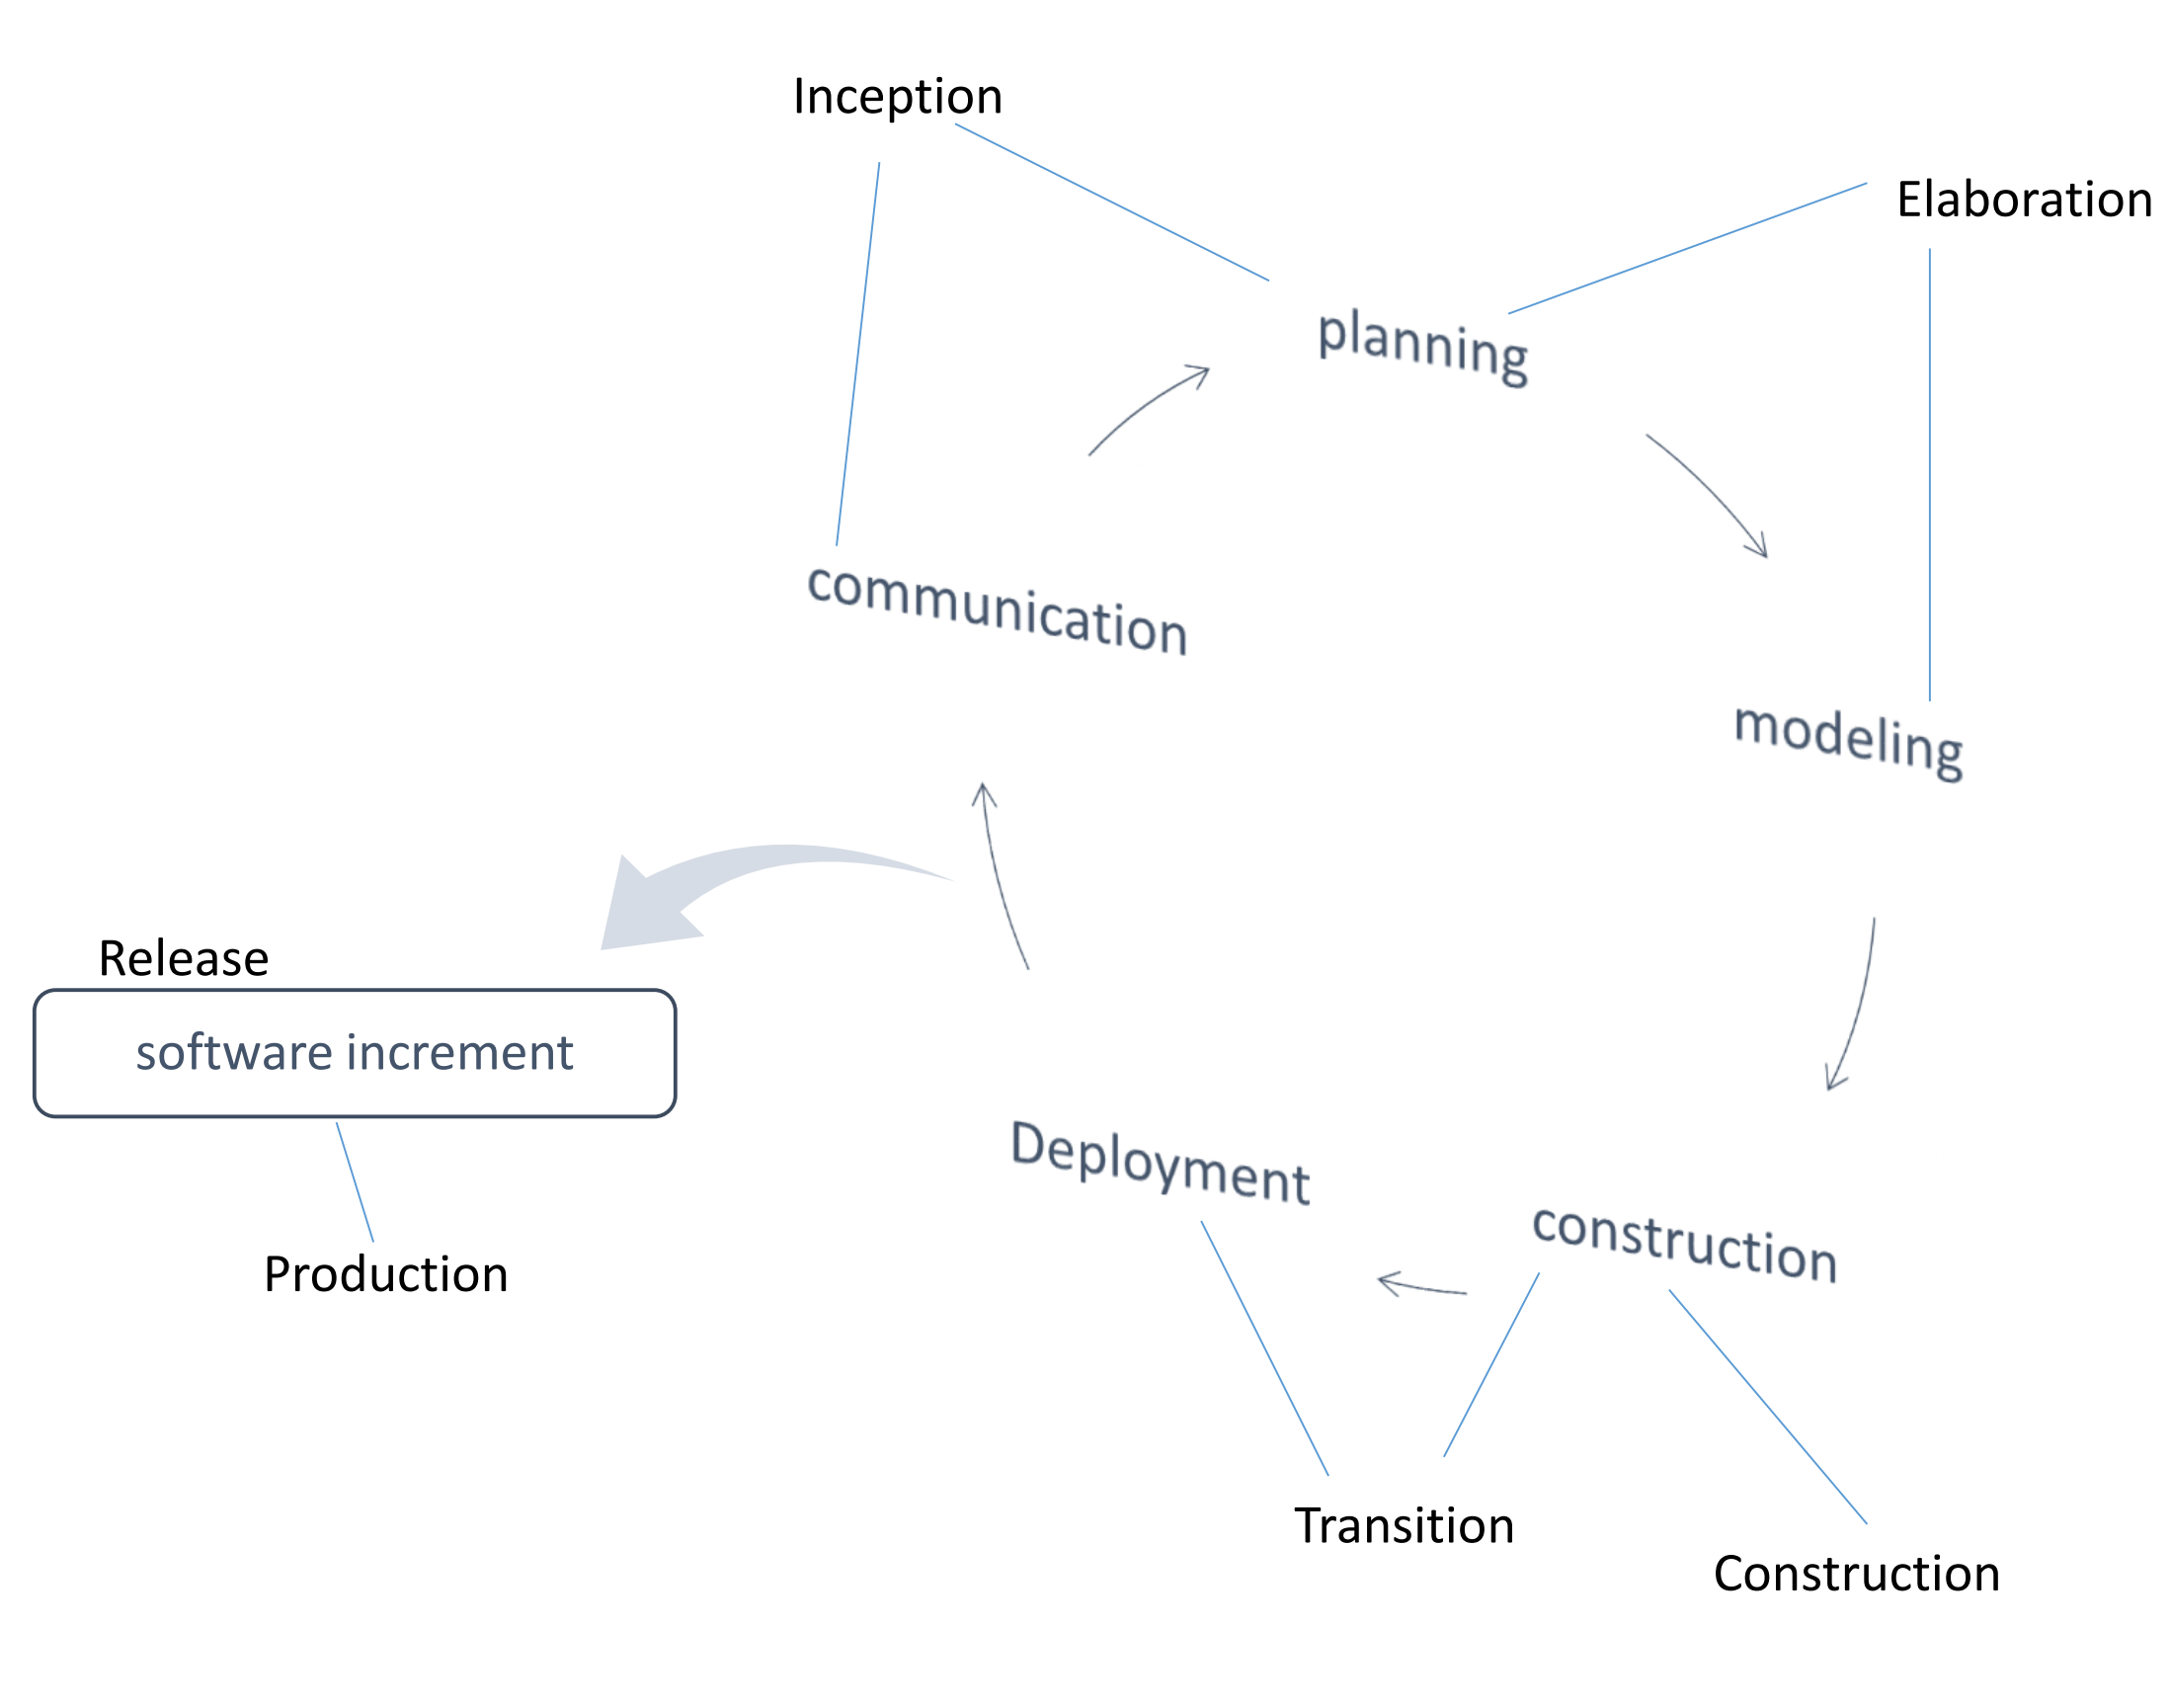
\includegraphics[width=1\textwidth]{pic/up_model.png}
	\end{center}
	\caption{Unified Process Model}
	\label{fig:up_model}
\end{figure}
\fi

\begin{figure}[h]
	\begin{center}
	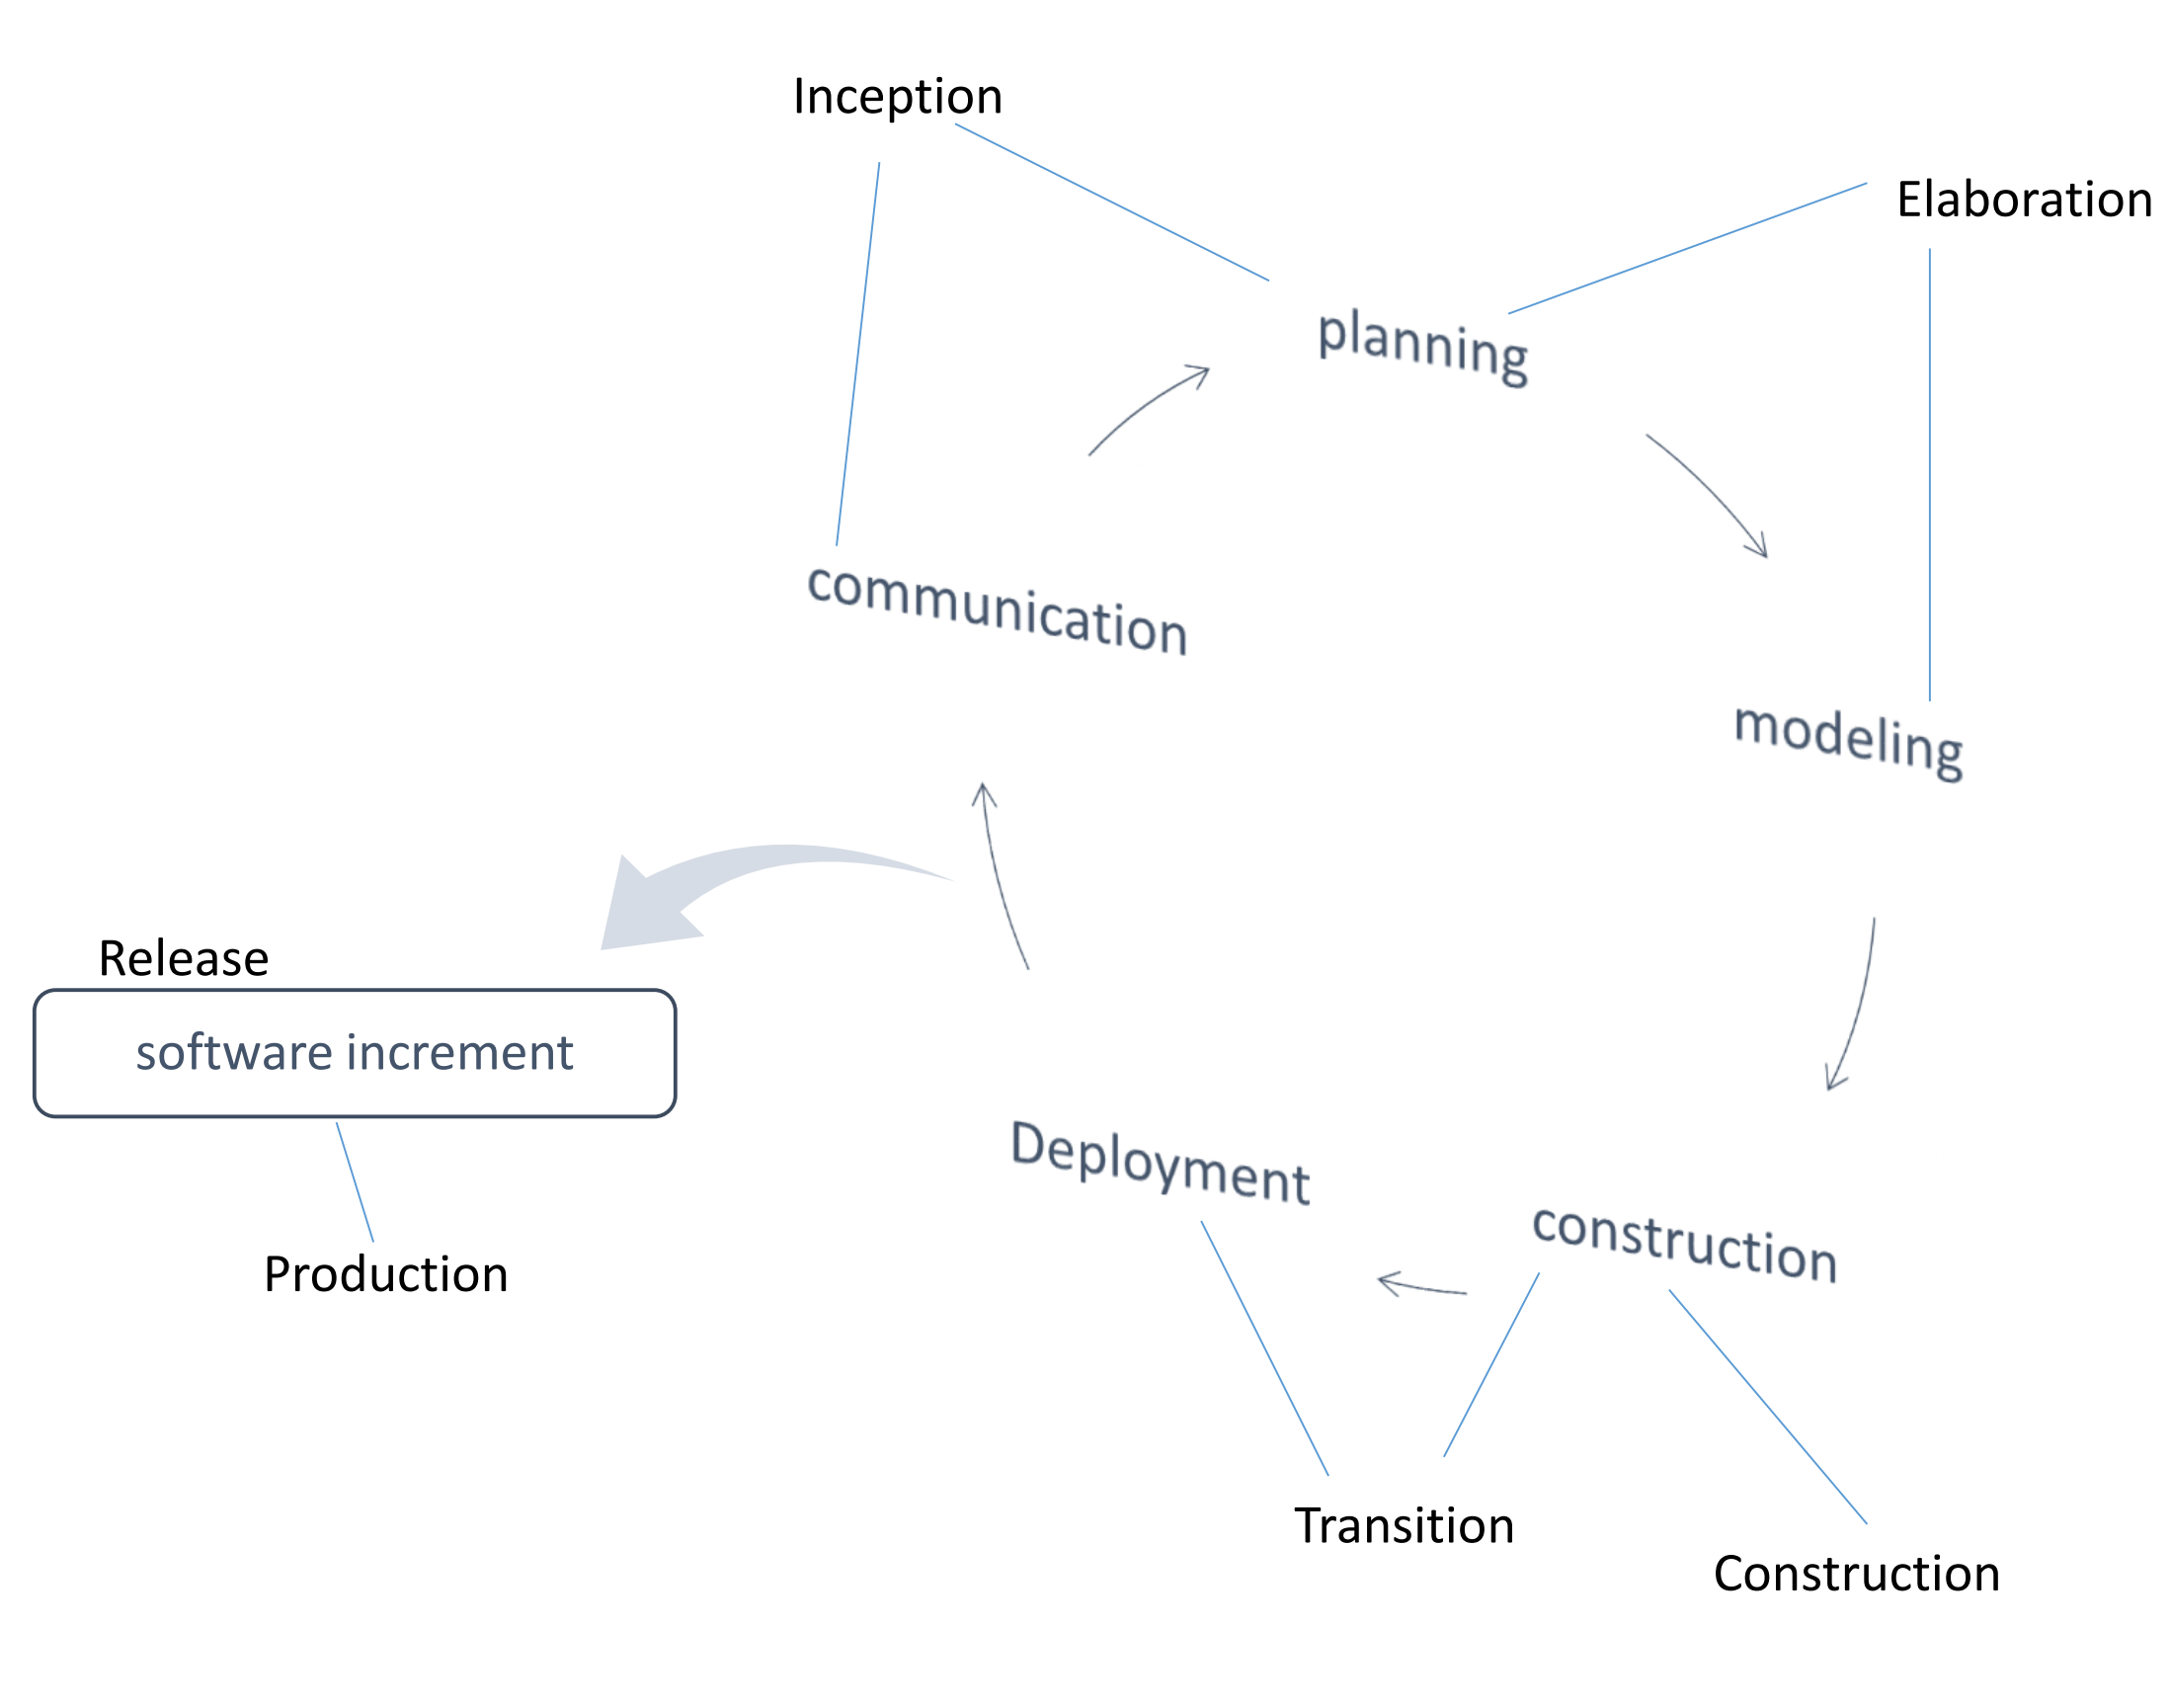
\includegraphics[width=0.5\textwidth]{pic/up_model.png}
	\end{center}
	%latex how to skip a figure in list of figure
	\caption[]{Unified Process Model}
	\label{fig:up_model}
\end{figure}
\clearpage


%\section{Problem Analysis}
%\section{Scheduling}

\section{Diagrams}
Diagrams gives the overview of the project and help develop efficient, effective and correct designs, particularly Object Oriented designs. Diagrams are also gives an environment to communicate clearly with project stakeholders (concerned parties:  developers, customer, etc).
UML diagrams are organized into two distinct groups: structural diagrams and behavioral or interaction diagrams.\\
%\clearpage

\renewcommand{\labelenumi}{\alph{enumi})}
\begin{enumerate}


	\item \textbf{Behavioral UML diagrams}
	\begin{enumerate}
		\item Use case diagram
		\item Activity diagram
	\end{enumerate}
	
	\item \textbf{Structural UML diagrams}
	\begin{enumerate}
		\item Class diagram
		\item Deployment diagram
	\end{enumerate}
	\item \textbf{ER-Diagram}
	\item \textbf{Schema Diagram}
	\item \textbf{Data Flow Diagram}
\end{enumerate}


\ifx
use cases.
class diagrams.
sequence diagrams.
package diagrams.
state diagrams
activity diagrams
deployment diagrams.

\fi


\subsection{Use Case Diagram}
Use Case Diagram referred to as behavior diagrams used to describe a set of actions or event steps defining the interactions between a role(actor) and a system to achieve a goal. The main purpose of a use case diagram is to exhibit who interacts with the system, and the main goals they can achieve with it.
In this project users are divided into several categories.
\renewcommand{\labelenumi}{\alph{enumi})}
\begin{enumerate}


		\item Administrator
		\item Requisitioner
		\item Approver
		\item Buyer
		\item Receiver
\end{enumerate}
%There are several usecase diagram has been generated for a better behavioral understanding of the project.


\begin{center}
\begin{figure}[h]
	\begin{center}
	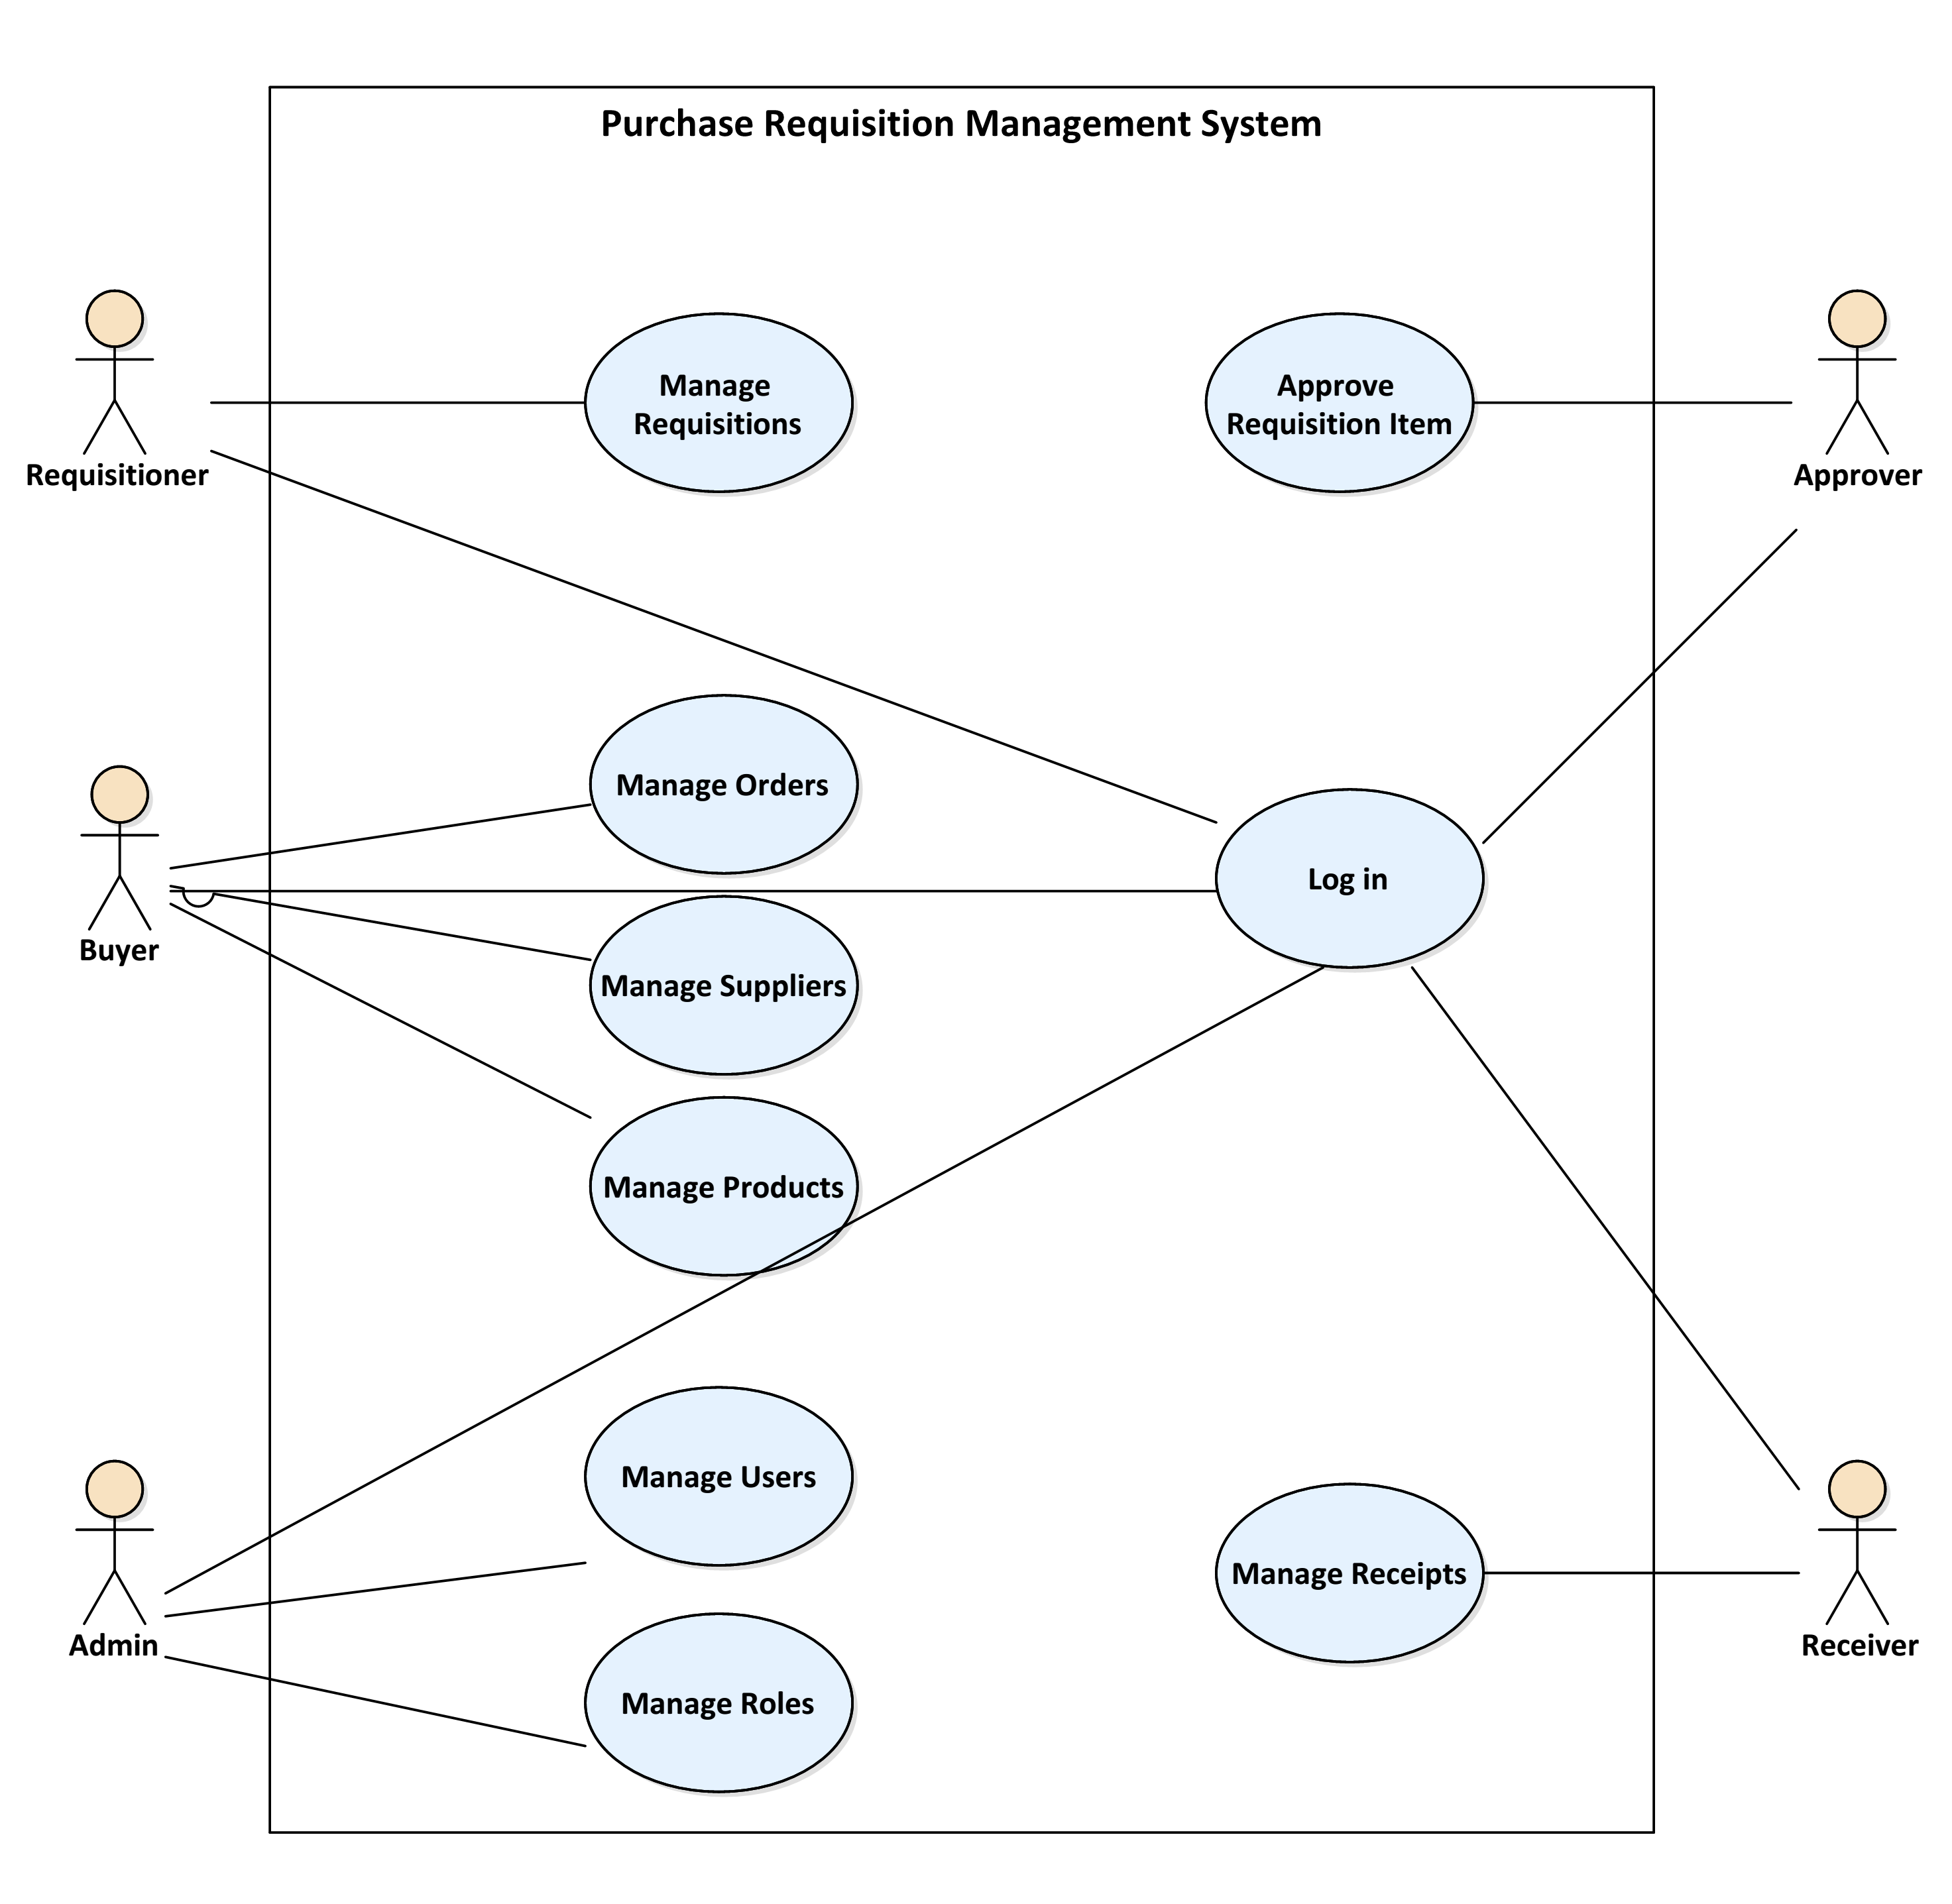
\includegraphics[width=1\textwidth]{pic/usecase/seupr_usecase_full.png}
	\end{center}
	\caption{SEU Purchase Requisition Use-case Diagram}
	\label{fig:seupr_usecase_full}
\end{figure}
\end{center}
\clearpage


\ifx
How Do You Write a Use Case?

Use cases contain the following elements:

Name – A clear verb/noun or actor/verb/noun descriptor that communicates the scope of the use case.
Brief Description – A brief paragraph of text describing the scope of the use case.
Actors – A list of the types of users who can engage in the activities described in the use case. Actor names should not correspond to job titles.
Preconditions – Anything the solution can assume to be true when the use case begins.
Basic Flow – The set of steps the actors take to accomplish the goal of the use case. A clear description of what the system does in response to each user action.
Alternate Flows – Capture the less common user/system interactions, such as being on a new computer and answering a security question.
Exception Flows – The things that can happen that prevent the user from achieving their goal, such as providing an incorrect username and password.
Post Conditions – Anything that must be true when the use case is complete.
\fi


\begin{table}
\begin{tabular}{|l|l|}
\hline
 Name & Purchase Requisition Management System \\
\hline
 ID & 1 \\
 \hline
 Description & 
 \vtop{
 		\hbox{\strut User wants to log-in, view profile, edit, change password and log-out}
		\hbox{\strut Admin wants to access user list and add user and assign roles}
		\hbox{\strut Admin wants to roles list and add new roles and assign user}
		\hbox{\strut Requisitioner wants to access the requisition list and add new requisition list}
		\hbox{\strut Requisitioner wants to view requisition items}
		\hbox{\strut Approver wants to approve or reject a requisition item}
		\hbox{\strut Buyer wants to access the order list and add new order list}
		\hbox{\strut Buyer wants to view requisition items}
		\hbox{\strut Receiver wants to access the receipt list and add new receipt list}
		\hbox{\strut Receiver wants to add new receipt item} 		
	}\\
\hline
  Actors & Admin, Requisitioner, Approver, Buyer, Receiver  \\
\hline
 Preconditions & User must have a valid account and have to log-in \\
 \hline

 Main Flow &  
		
	\vtop{
 		\hbox{\strut User log-in the system and performs with specific roles }
		\hbox{\strut Admin add user , roles and assign roles the the users}
		\hbox{\strut Requisitioner access the requisition list and add new requisition list \& items}
		\hbox{\strut Approver approves or rejects a requisition item by analysis}
		\hbox{\strut Buyer access the order list, add new order list, items, schedules \& distributions}
		\hbox{\strut Receiver access the receipt list, add new receipt list \& items}
	}\\		
 \hline
  Postconditions & 
  \vtop{
 		\hbox{\strut The system creates new roles, new users, assign roles}
		\hbox{\strut System generates new requisition list and items and approved}
		\hbox{\strut System generates new order list and items, schedules and distributions}
		\hbox{\strut System generates new receive list and items }		
	}\\
\hline
% Alternative Flow & 2 \\
%\hline
% 
\end{tabular}
\end{table}
\clearpage


% all usecase commenting================
% all usecase commenting================

\ifx

\begin{center}
\begin{figure}[h]
	\begin{center}
	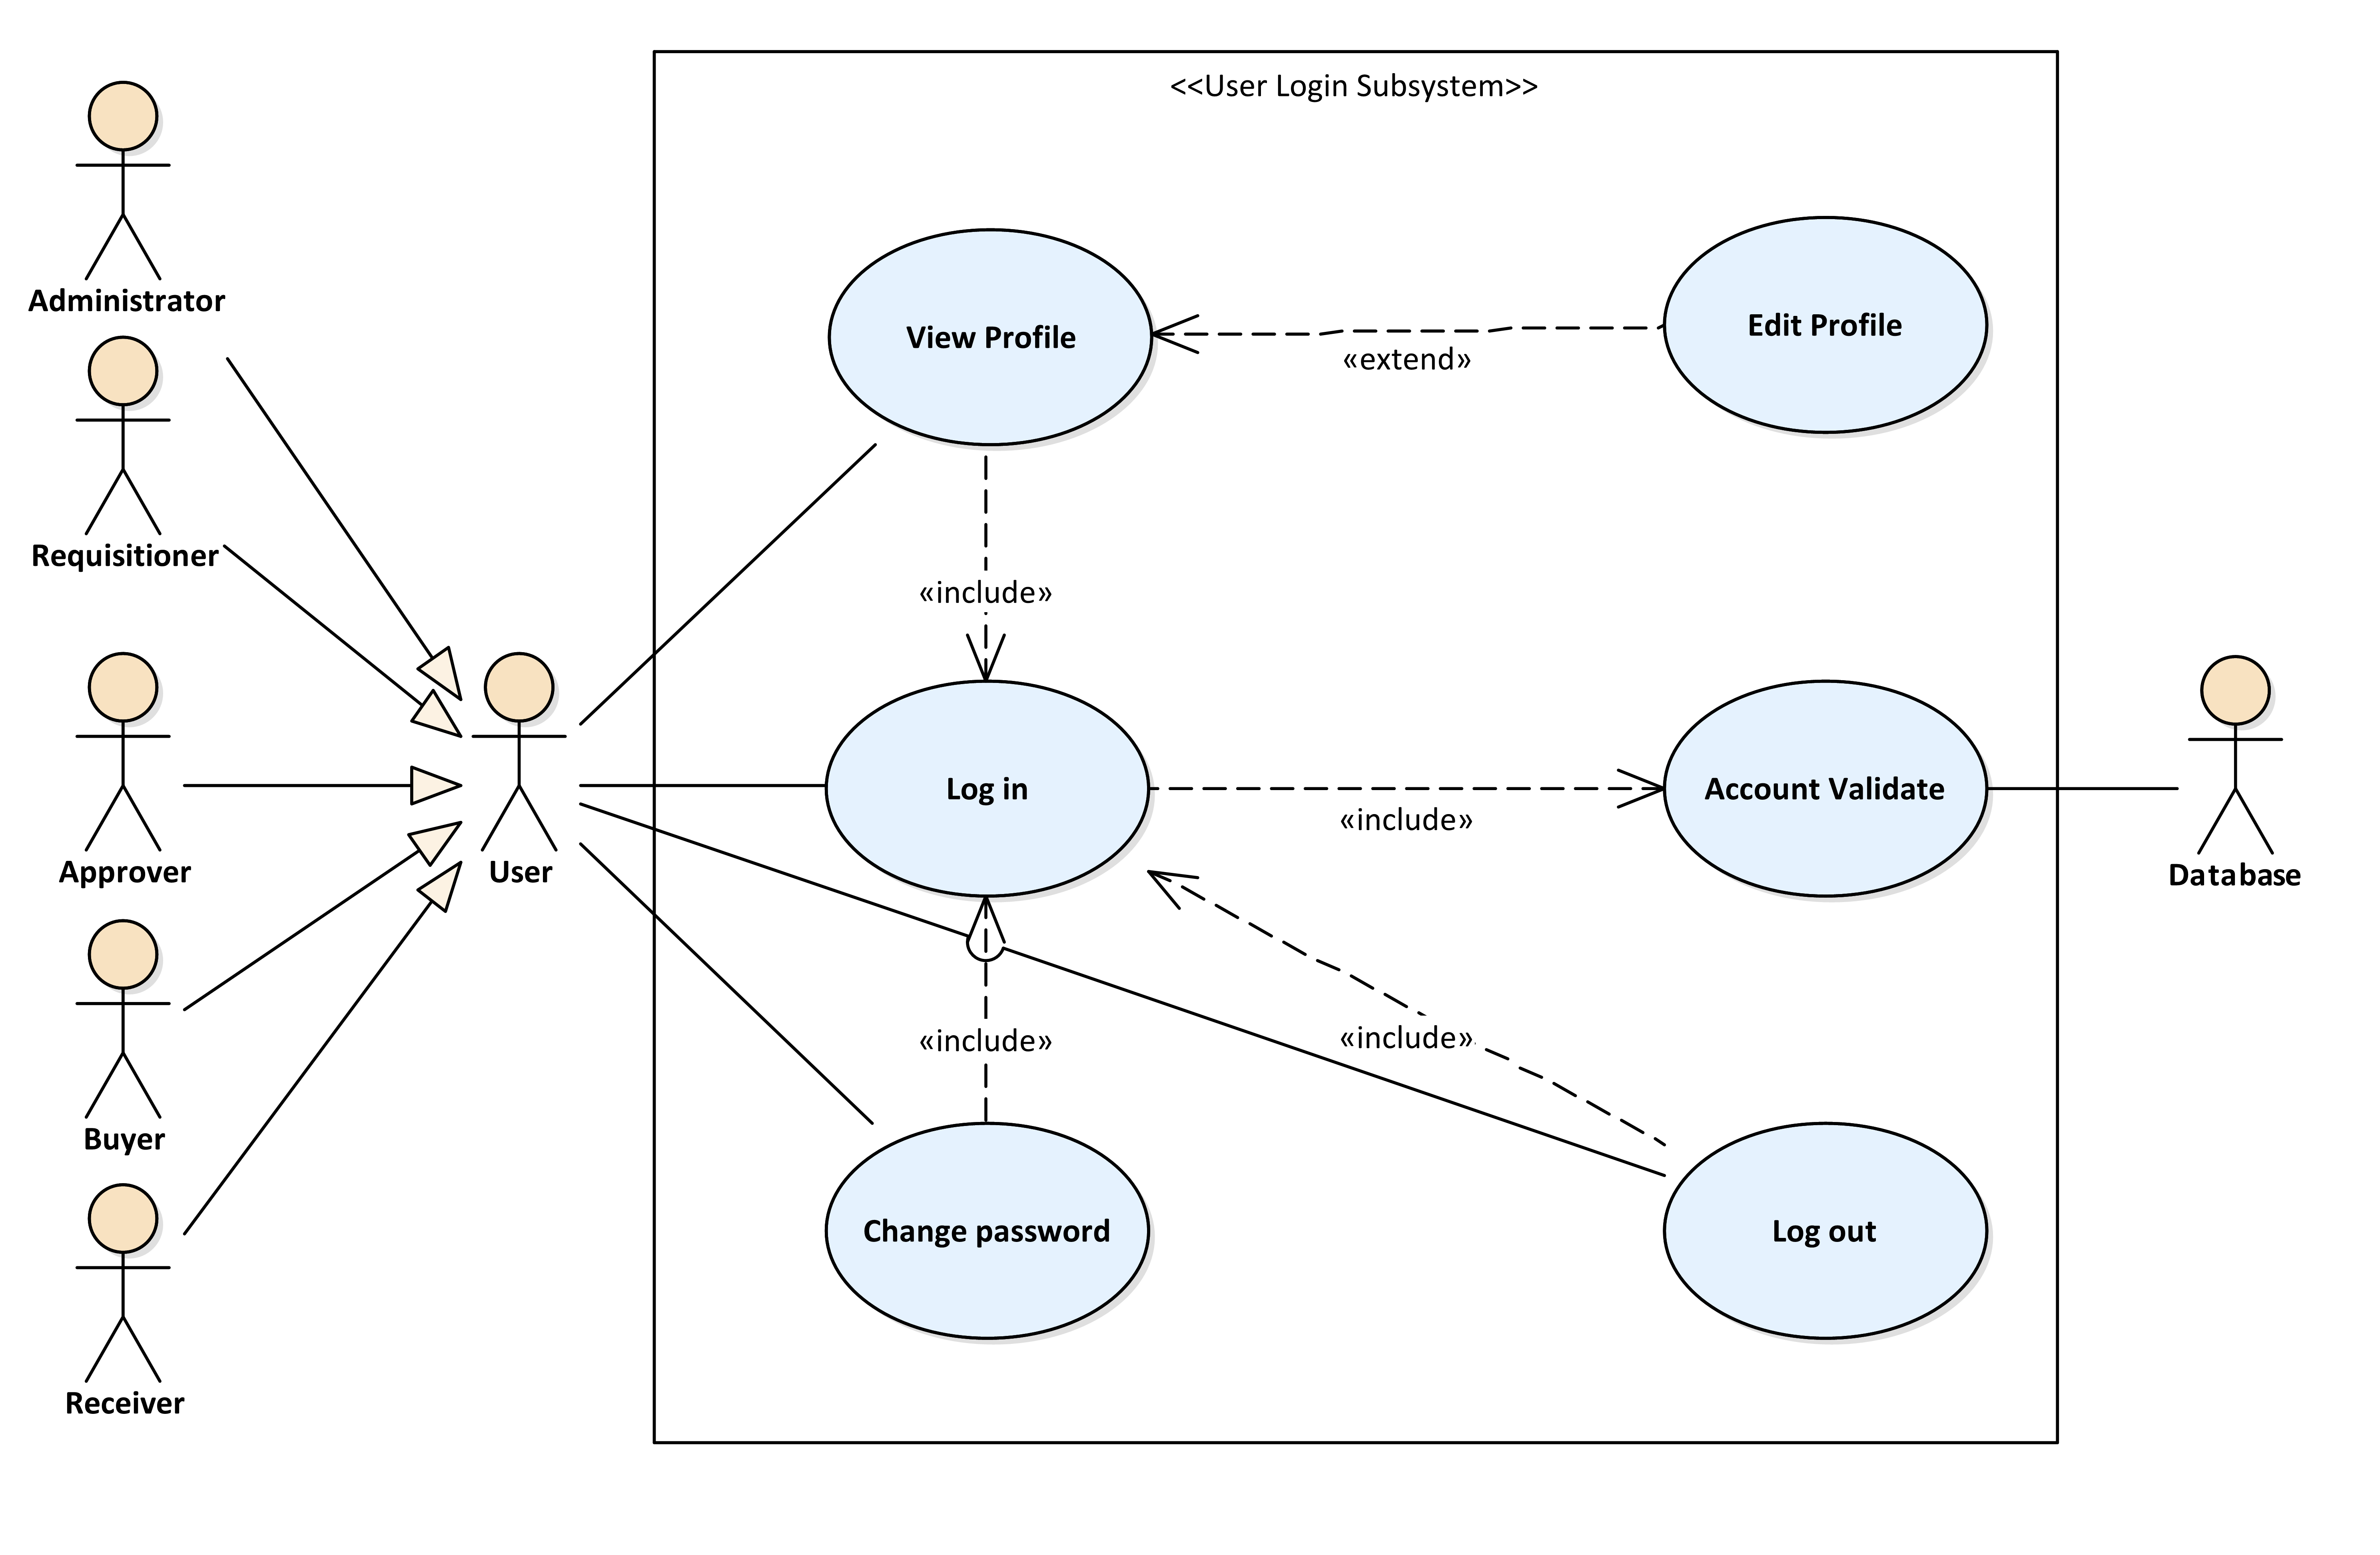
\includegraphics[width=.8\textwidth]{pic/usecase/seupr_usecase_login.png}
	\end{center}
	\caption{Log-in Use-case Diagram}
	\label{fig:seupr_usecase_login}
\end{figure}
\end{center}

\fi
% all usecase commenting================
% all usecase commenting================


\ifx
%https://www.youtube.com/watch?v=i3dg99MWLZU

\begin{tabular}{|l|l|}
\hline
 Name & 2 \\
\hline
 ID & 2 \\
 \hline
 Description & 2 \\
\hline
 Primary Actor & 2 \\
 \hline
 Secondary Actor & 2 \\
\hline
 Preconditions & 2 \\
 \hline
 Postconditions & 2 \\
\hline
 Main Flow & 2 \\
 \hline
 Alternative Flow & 2 \\
\hline
 
\end{tabular}
\fi

% all usecase commenting================
% all usecase commenting================

\ifx

\begin{table}
\begin{tabular}{|l|l|}
\hline
 Name & Login \\
\hline
 ID & UC-1 \\
 \hline
 Description & 
 \vtop{
 		\hbox{\strut User wants to access the system via log-in}				\hbox{\strut User wants to view profile and edit}
 		\hbox{\strut User wants to change password}
 		\hbox{\strut User wants to logout }
	}\\
\hline
 Primary Actor & User \\
 \hline
 Secondary Actor & Database \\
\hline
 Preconditions & User must have a valid account \\
 \hline
 Postconditions & The system displays the relevant page\\
\hline
 Main Flow &  
		
	\vtop{
 		\hbox{\strut User enters username and password}	
 		\hbox{\strut User submit username and password}
 		\hbox{\strut Database validates the username and password}	
 		\hbox{\strut User enters homepage}
 		\hbox{\strut User view profile page and edits and save}
 		\hbox{\strut User enters password change page and change password}
 		\hbox{\strut User logs out form the system}
 		\hbox{\strut Usecase ends}			
 								
	}\\		
 \hline
% Alternative Flow & 2 \\
%\hline
% 
\end{tabular}
\end{table}


%System Administration Use-case Diagram----------------
%System Administration Use-case Diagram----------------
\begin{center}
\begin{figure}[h]
	\begin{center}
	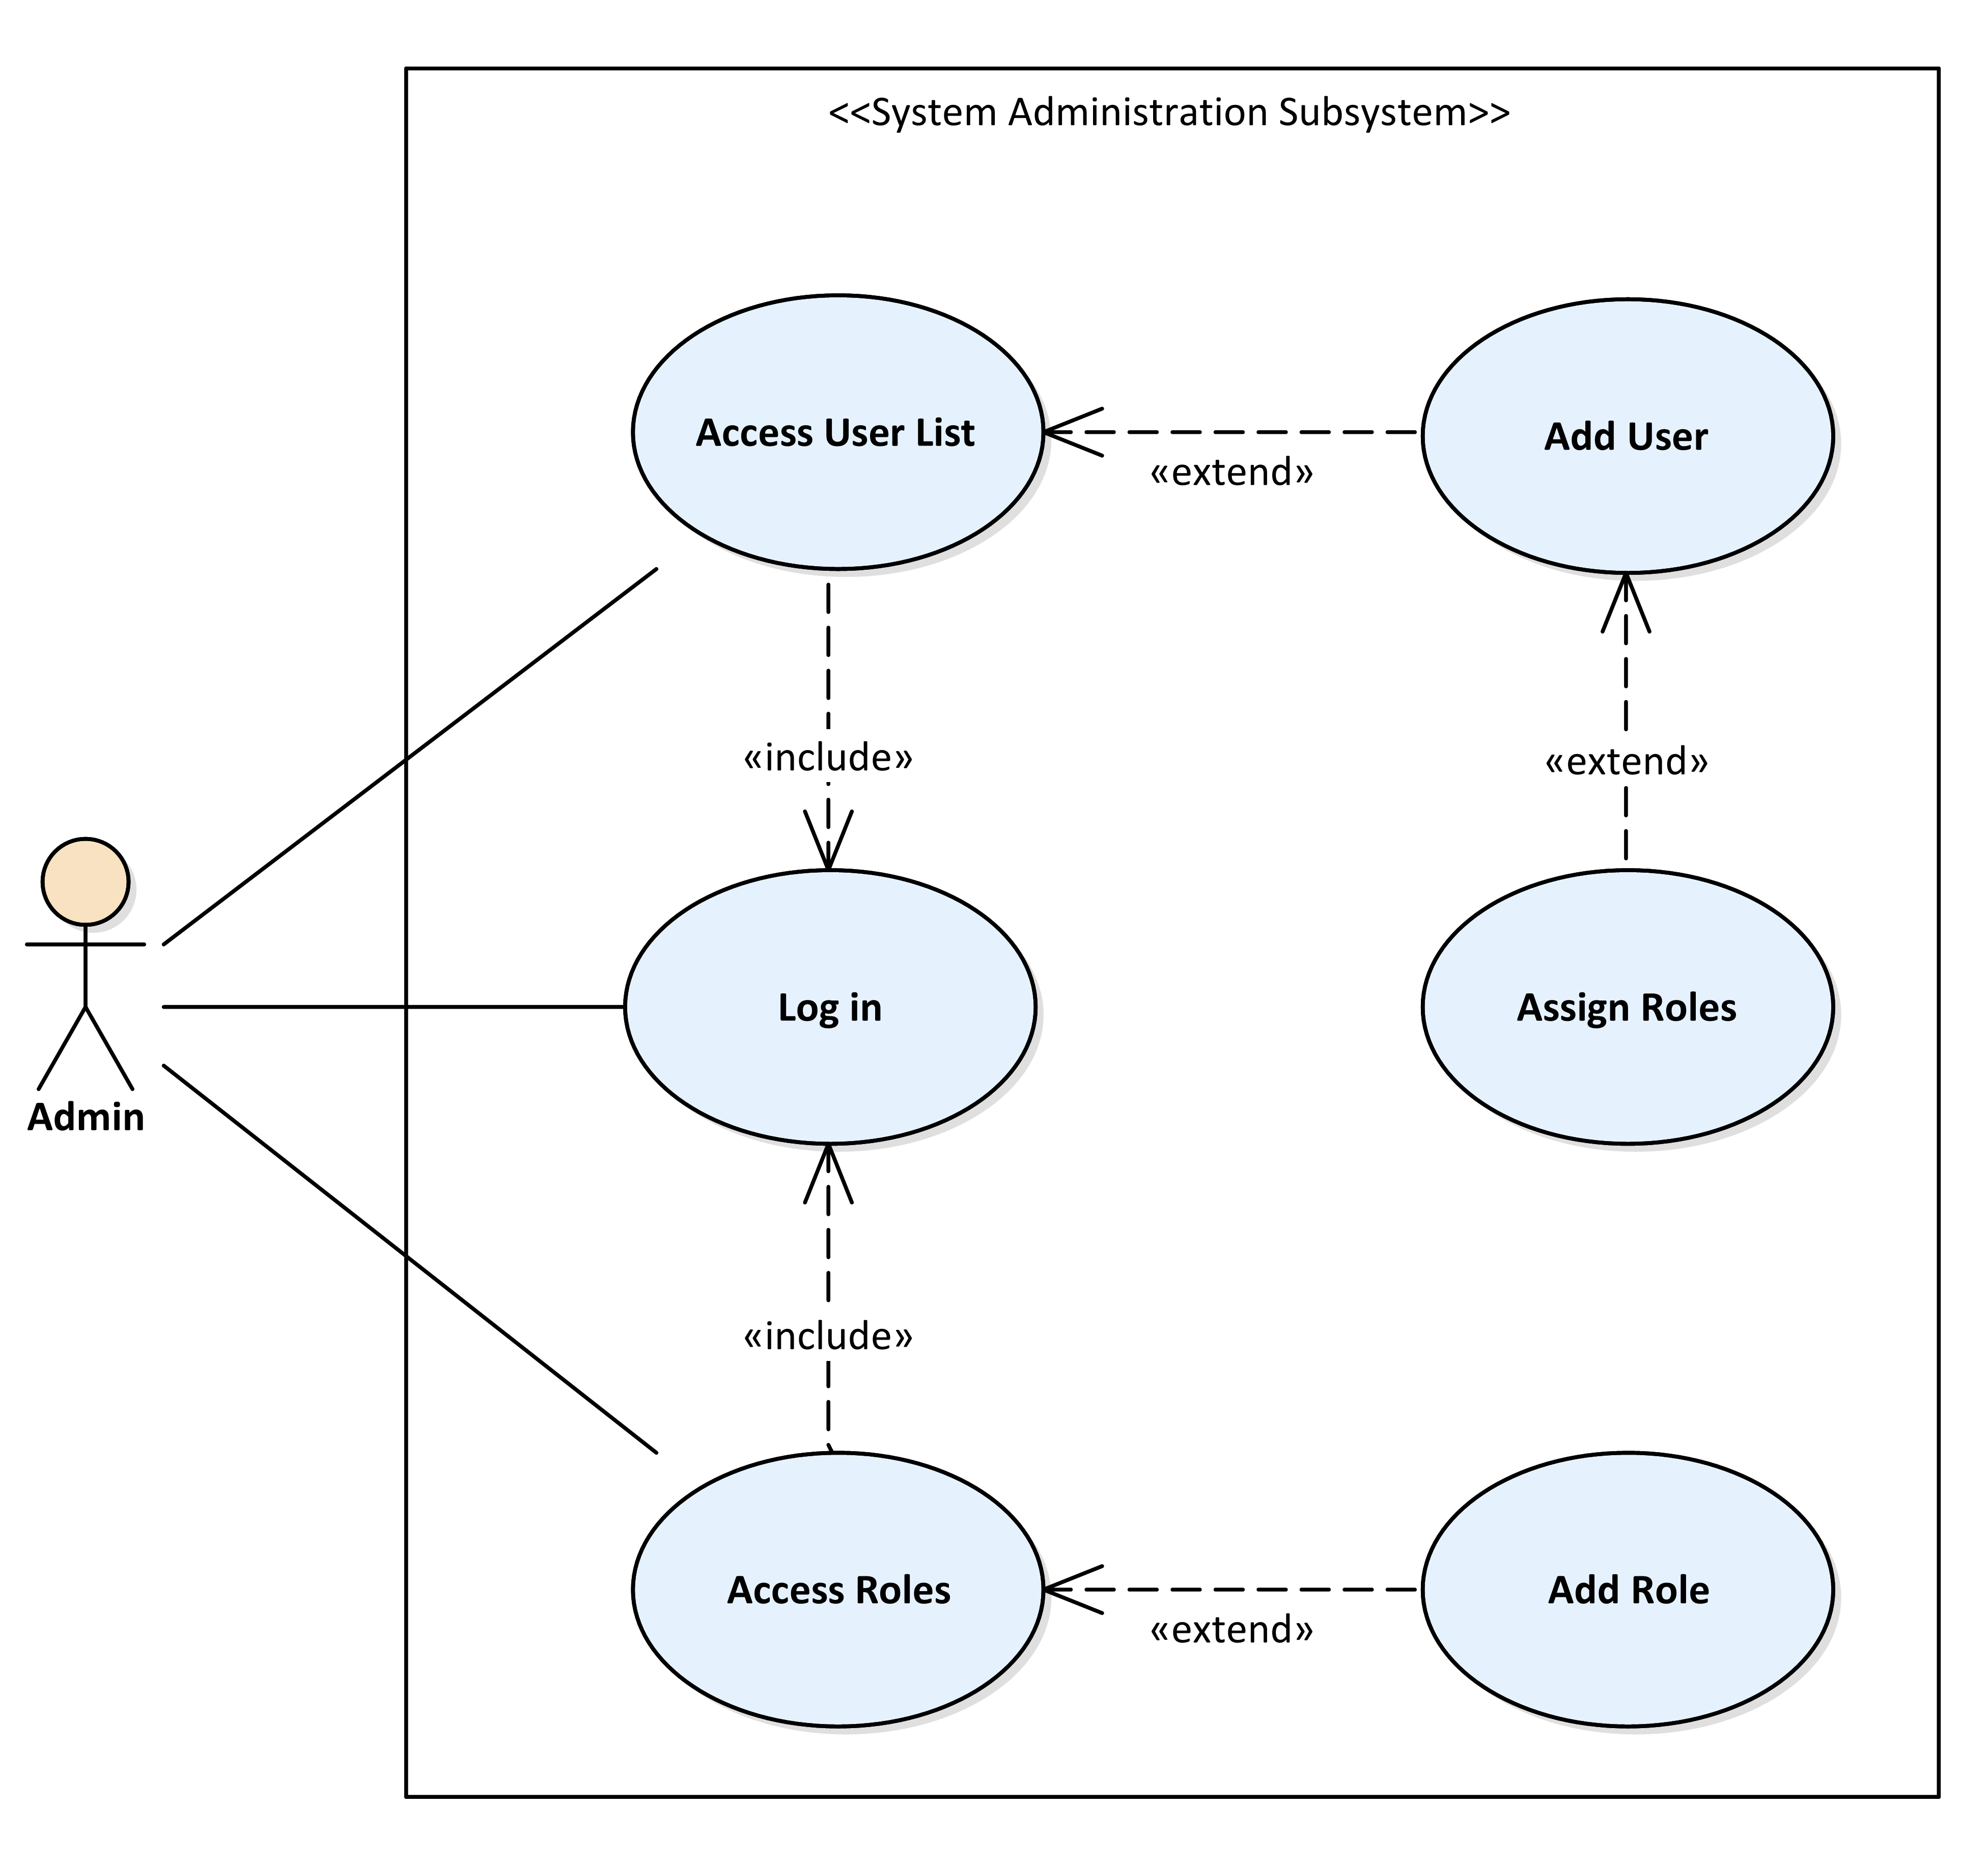
\includegraphics[width=.7\textwidth]{pic/usecase/seupr_usecase_administration.png}
	\end{center}
	\caption{Administration Use-case Diagram}
	\label{fig:seupr_usecase_administration}
\end{figure}
\end{center}
\clearpage
\begin{table}
\begin{tabular}{|l|l|}
\hline
 Name & Administration \\
\hline
 ID & UC-2 \\
 \hline
 Description & 
 \vtop{
 		\hbox{\strut Admin wants to access user list and add user and assign roles}				
 		\hbox{\strut Admin wants to roles list and add new roles and assign user}

	}\\
\hline
 Primary Actor & Admin \\
 \hline
 Secondary Actor & None \\
\hline
 Preconditions & Admin must log-in and must have ``Add user" and  ``Add user" roles\\
 \hline
 Postconditions & The system creates new roles and new users\\
\hline
 Main Flow &  
		
	\vtop{
 		\hbox{\strut Admin log-in the system}	
 		\hbox{\strut Admin access user list}
 		\hbox{\strut Admin creates new user}	
 		\hbox{\strut Admin access role list}
 		\hbox{\strut Admin creates new roles}
 		\hbox{\strut Admin assigns users to the roles}
 		\hbox{\strut Usecase ends}			 								
	}\\		
 \hline
\end{tabular}
\end{table}










%Purchase Requisition Use-case Diagram----------------
%Purchase Requisition Use-case Diagram----------------
\begin{figure}[h]
	\begin{center}
	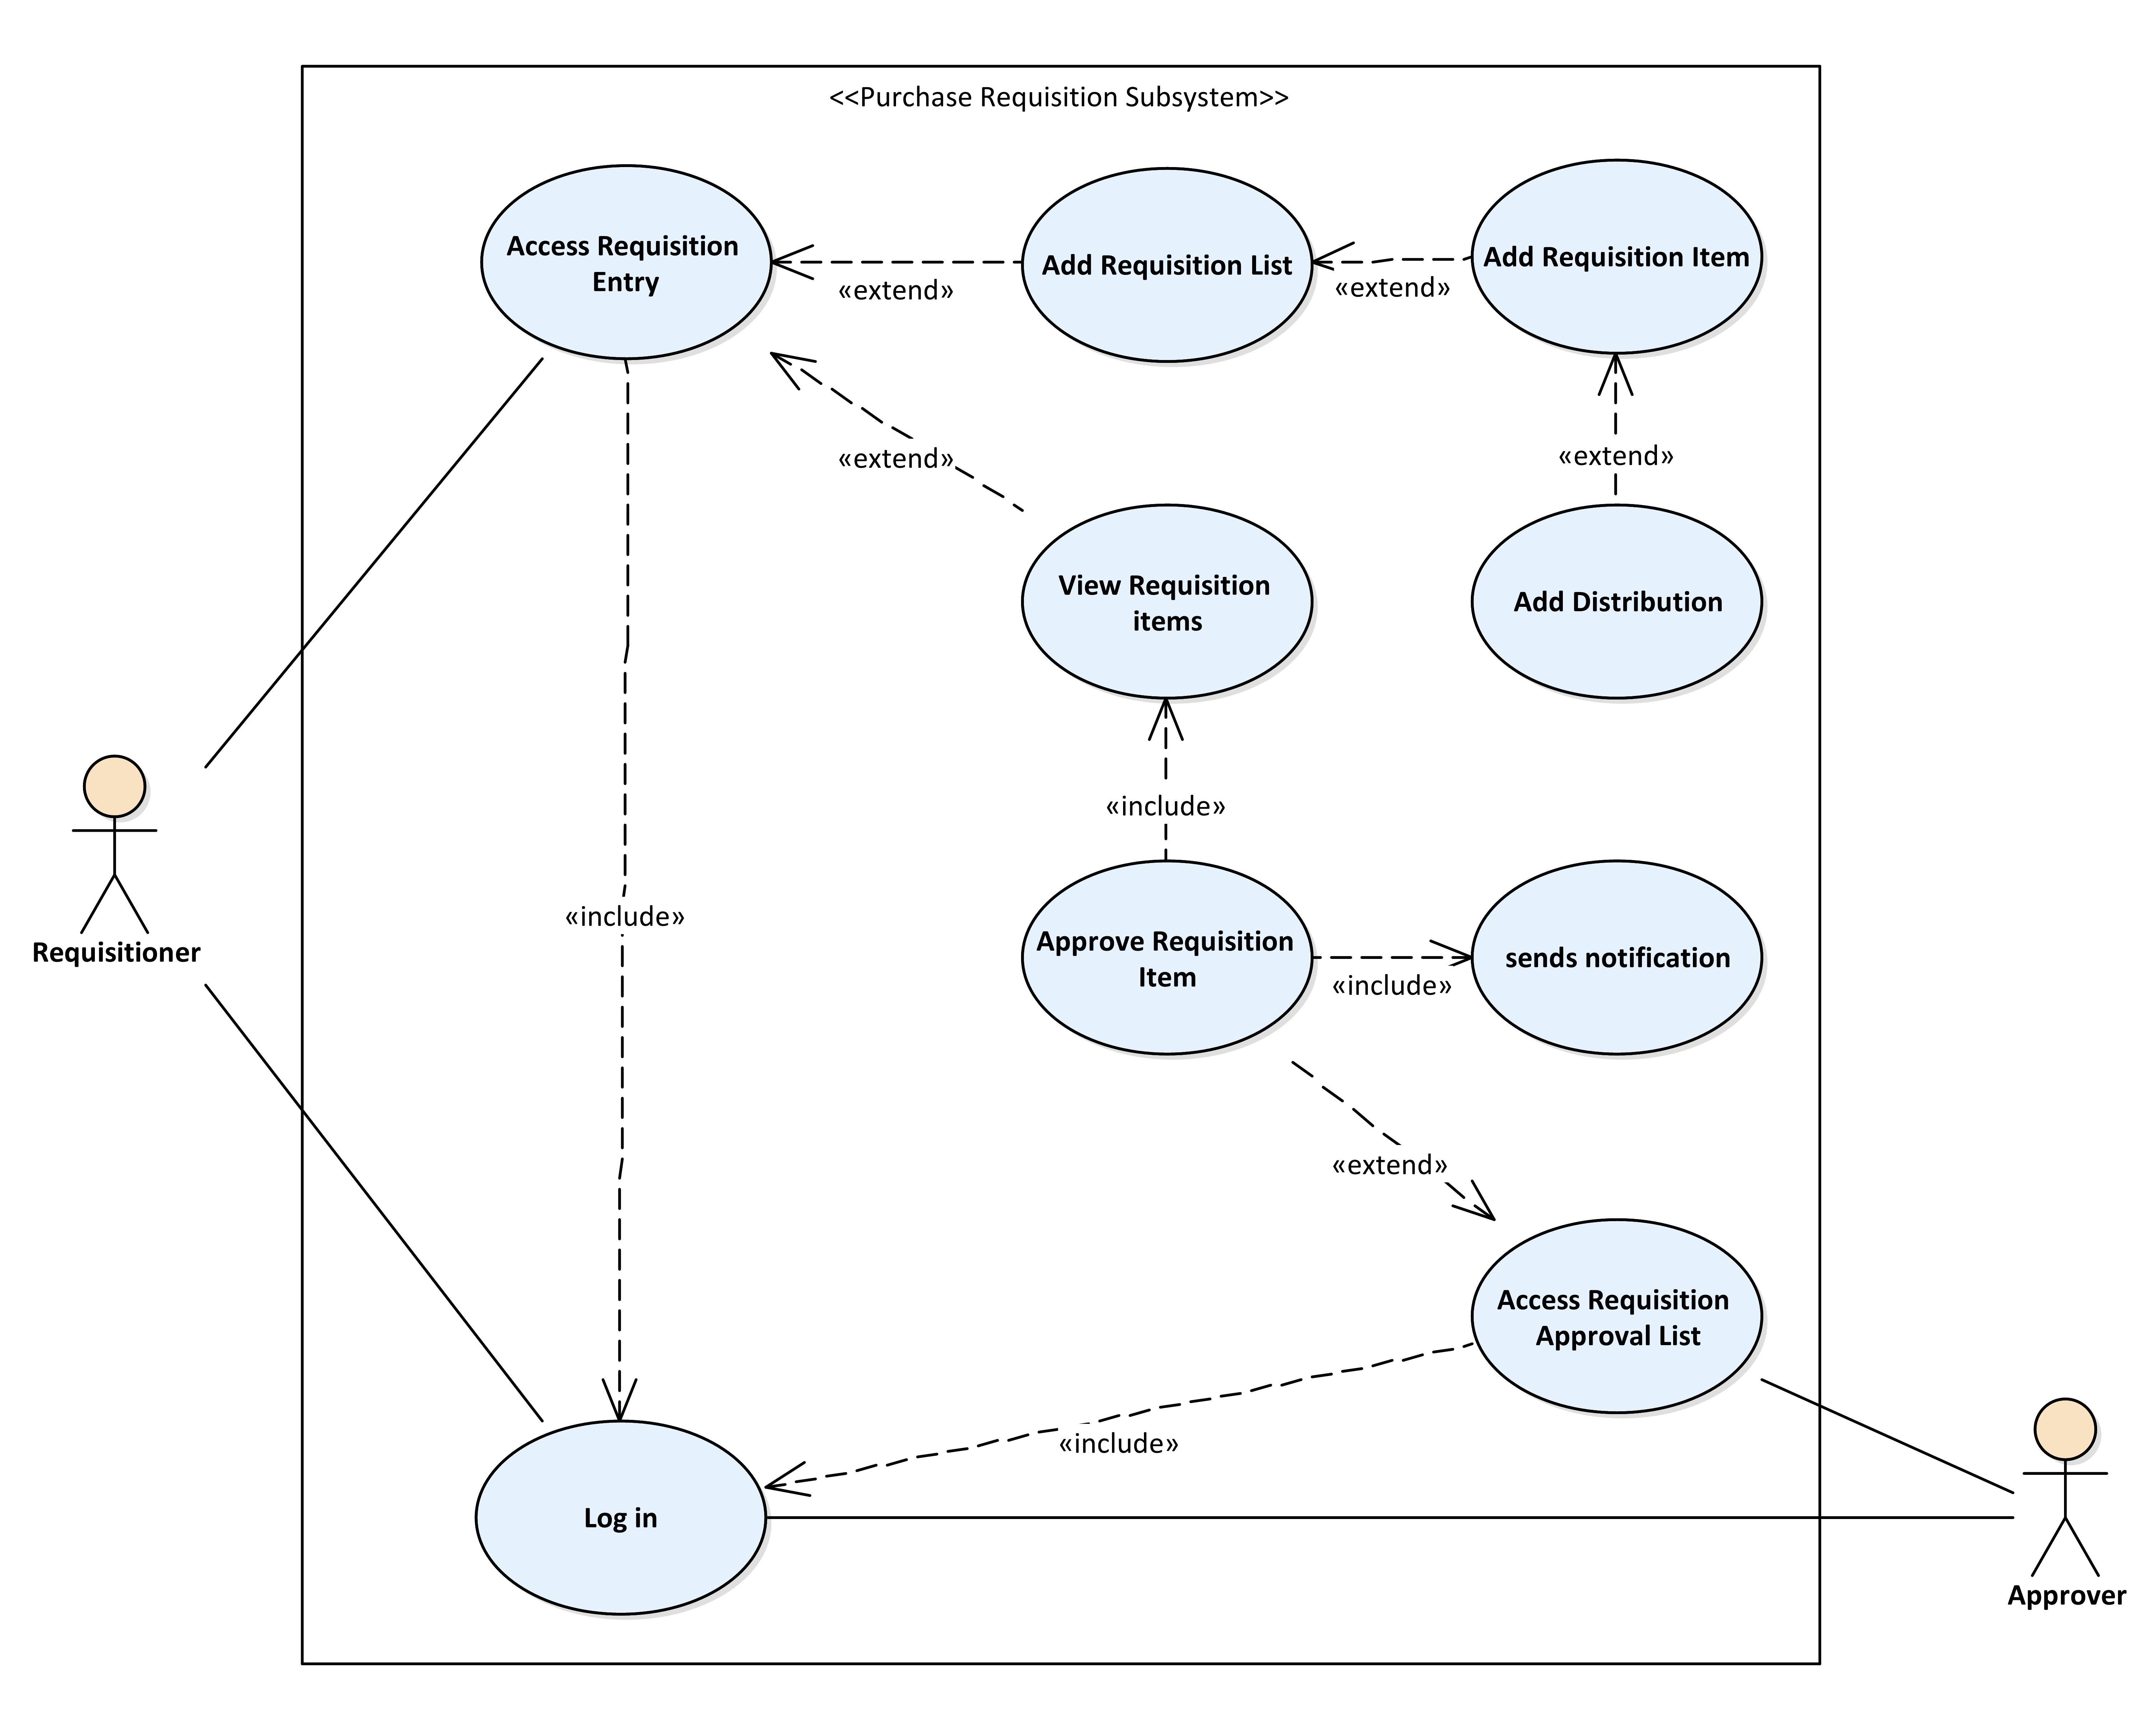
\includegraphics[width=1\textwidth]{pic/usecase/seupr_usecase_requisitioner.png}
	\end{center}
	\caption{Purcase Requisition Use-case Diagram}
	\label{fig:seupr_usecase_requisitioner}
\end{figure}
\clearpage



\begin{table}
\begin{tabular}{|l|l|}
\hline
 Name & Purchase Requisition \\
\hline
 ID & UC-3 \\
 \hline
 Description & 
 \vtop{
 		\hbox{\strut Requisitioner wants to access the requisition list and add new requisition list}				
 		\hbox{\strut Requisitioner wants to view requisition items}
 		\hbox{\strut Approver wants to approve or reject a requisition item}

	}\\
\hline
 Primary Actor & Requisitioner \\
 \hline
 Secondary Actor & Approver \\
\hline
 Preconditions & Requisitiner and approver must log-in the system and have the required roles\\
 \hline
 Postconditions & System generates new requisition list and items and approved\\
\hline
 Main Flow &  
		
	\vtop{
 		\hbox{\strut Requisitioner log-in the system}	
 		\hbox{\strut Requisitioner access requisition list}
 		\hbox{\strut Requisitioner creates new requisition list}
 		\hbox{\strut Requisitioner creates new requisition items}
 		\hbox{\strut Requisitioner creates new requisition distributions}	
 		
 		\hbox{\strut Approver log-in the system}	
 		\hbox{\strut Approver access requisition approval list}
 		\hbox{\strut Approver approves or rejects requisition items}	
 		
 		\hbox{\strut Usecase ends}			 								
	}\\		
 \hline
\end{tabular}
\end{table}








%Purchase Order Use-case Diagram----------------
%Purchase Order Use-case Diagram----------------
\begin{figure}[h]
	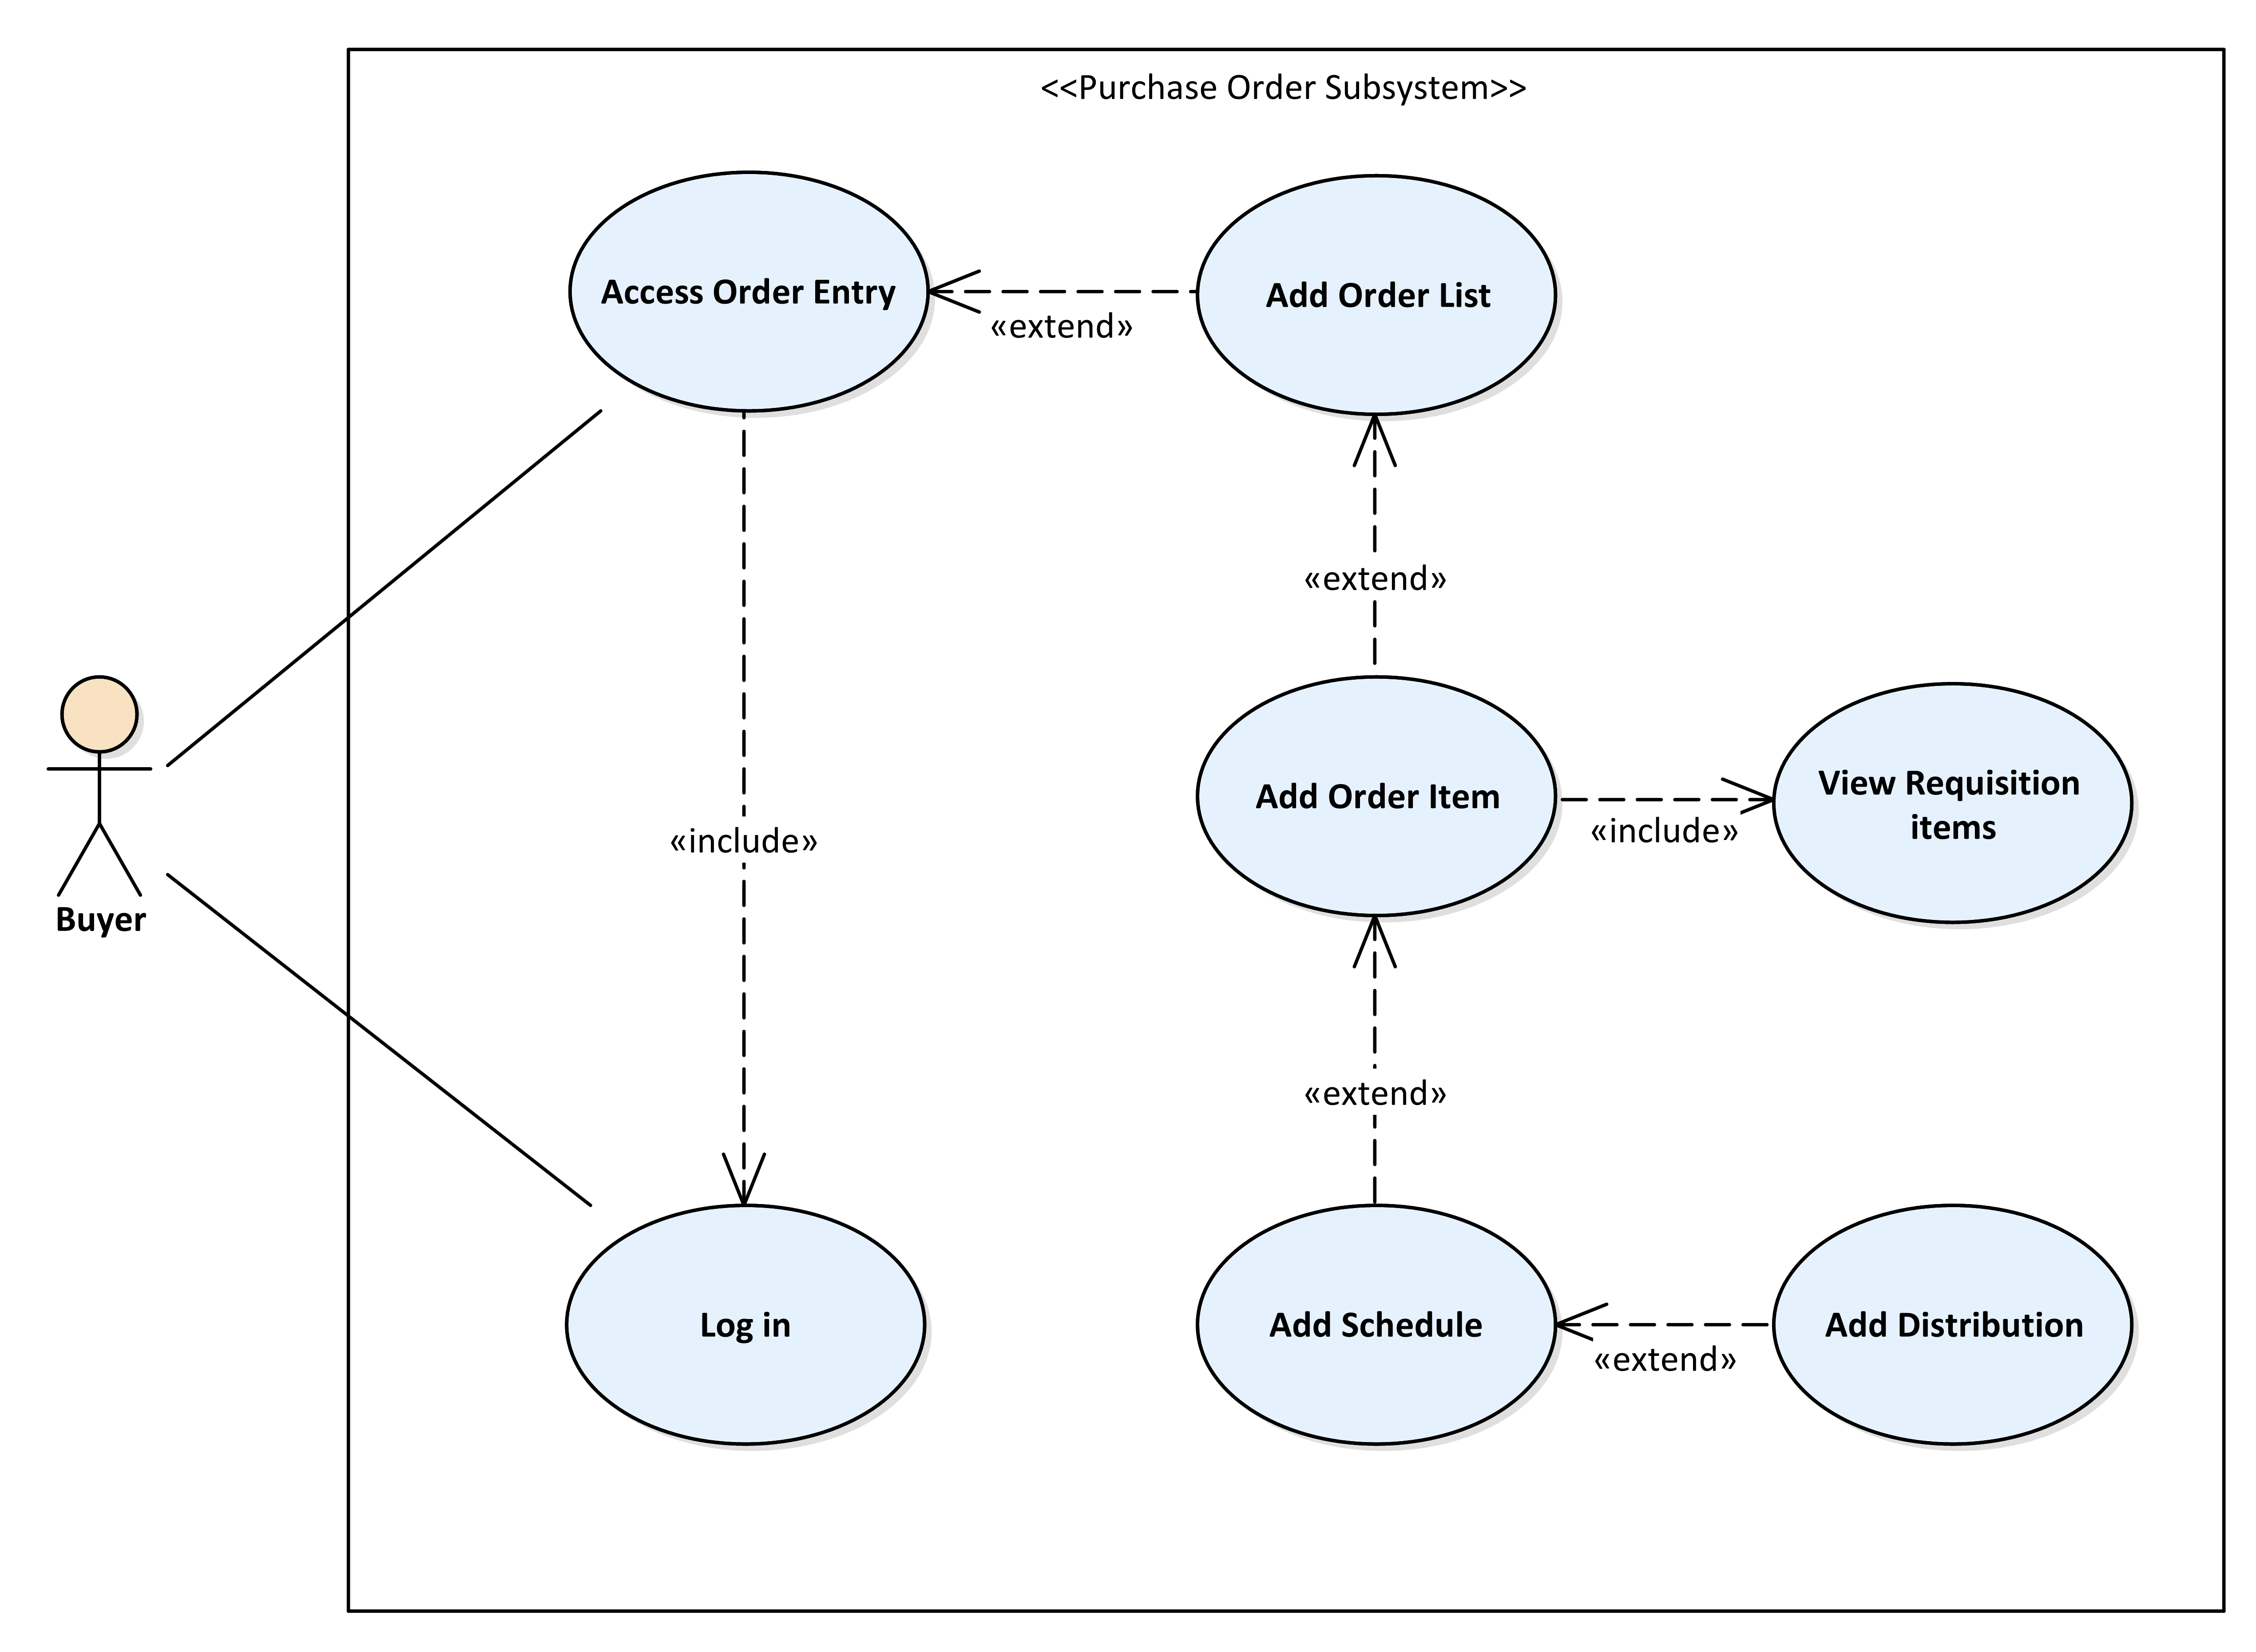
\includegraphics[width=.8\textwidth]{pic/usecase/seupr_usecase_buyer.png}
	\caption{Purcase Order Use-case Diagram}
	\label{fig:seupr_usecase_buyer}
\end{figure}


\begin{table}
\begin{tabular}{|l|l|}
\hline
 Name & Purchase Order \\
\hline
 ID & UC-4 \\
 \hline
 Description & 
 \vtop{
 		\hbox{\strut Buyer wants to access the order list and add new order list}				
 		\hbox{\strut Buyer wants to view requisition items}

	}\\
\hline
 Primary Actor & Buyer \\
 \hline
 Secondary Actor & None \\
\hline
 Preconditions & Buyer must log-in the system and have the required roles\\
 \hline
 Postconditions & System generates new order list and items \\
\hline
 Main Flow &  
		
	\vtop{
 		\hbox{\strut Buyer log-in the system}	
 		\hbox{\strut Buyer access order list}
 		\hbox{\strut Buyer creates new order list}
 		\hbox{\strut Buyer creates new order items}
 		\hbox{\strut Buyer creates new requisition shipment schedules}
 		\hbox{\strut Buyer creates new requisition distributions}	

 		\hbox{\strut Usecase ends}			 								
	}\\		
 \hline
\end{tabular}
\end{table}












%Purchase receive Use-case Diagram----------------
%Purchase receive Use-case Diagram----------------
\begin{figure}[h]
	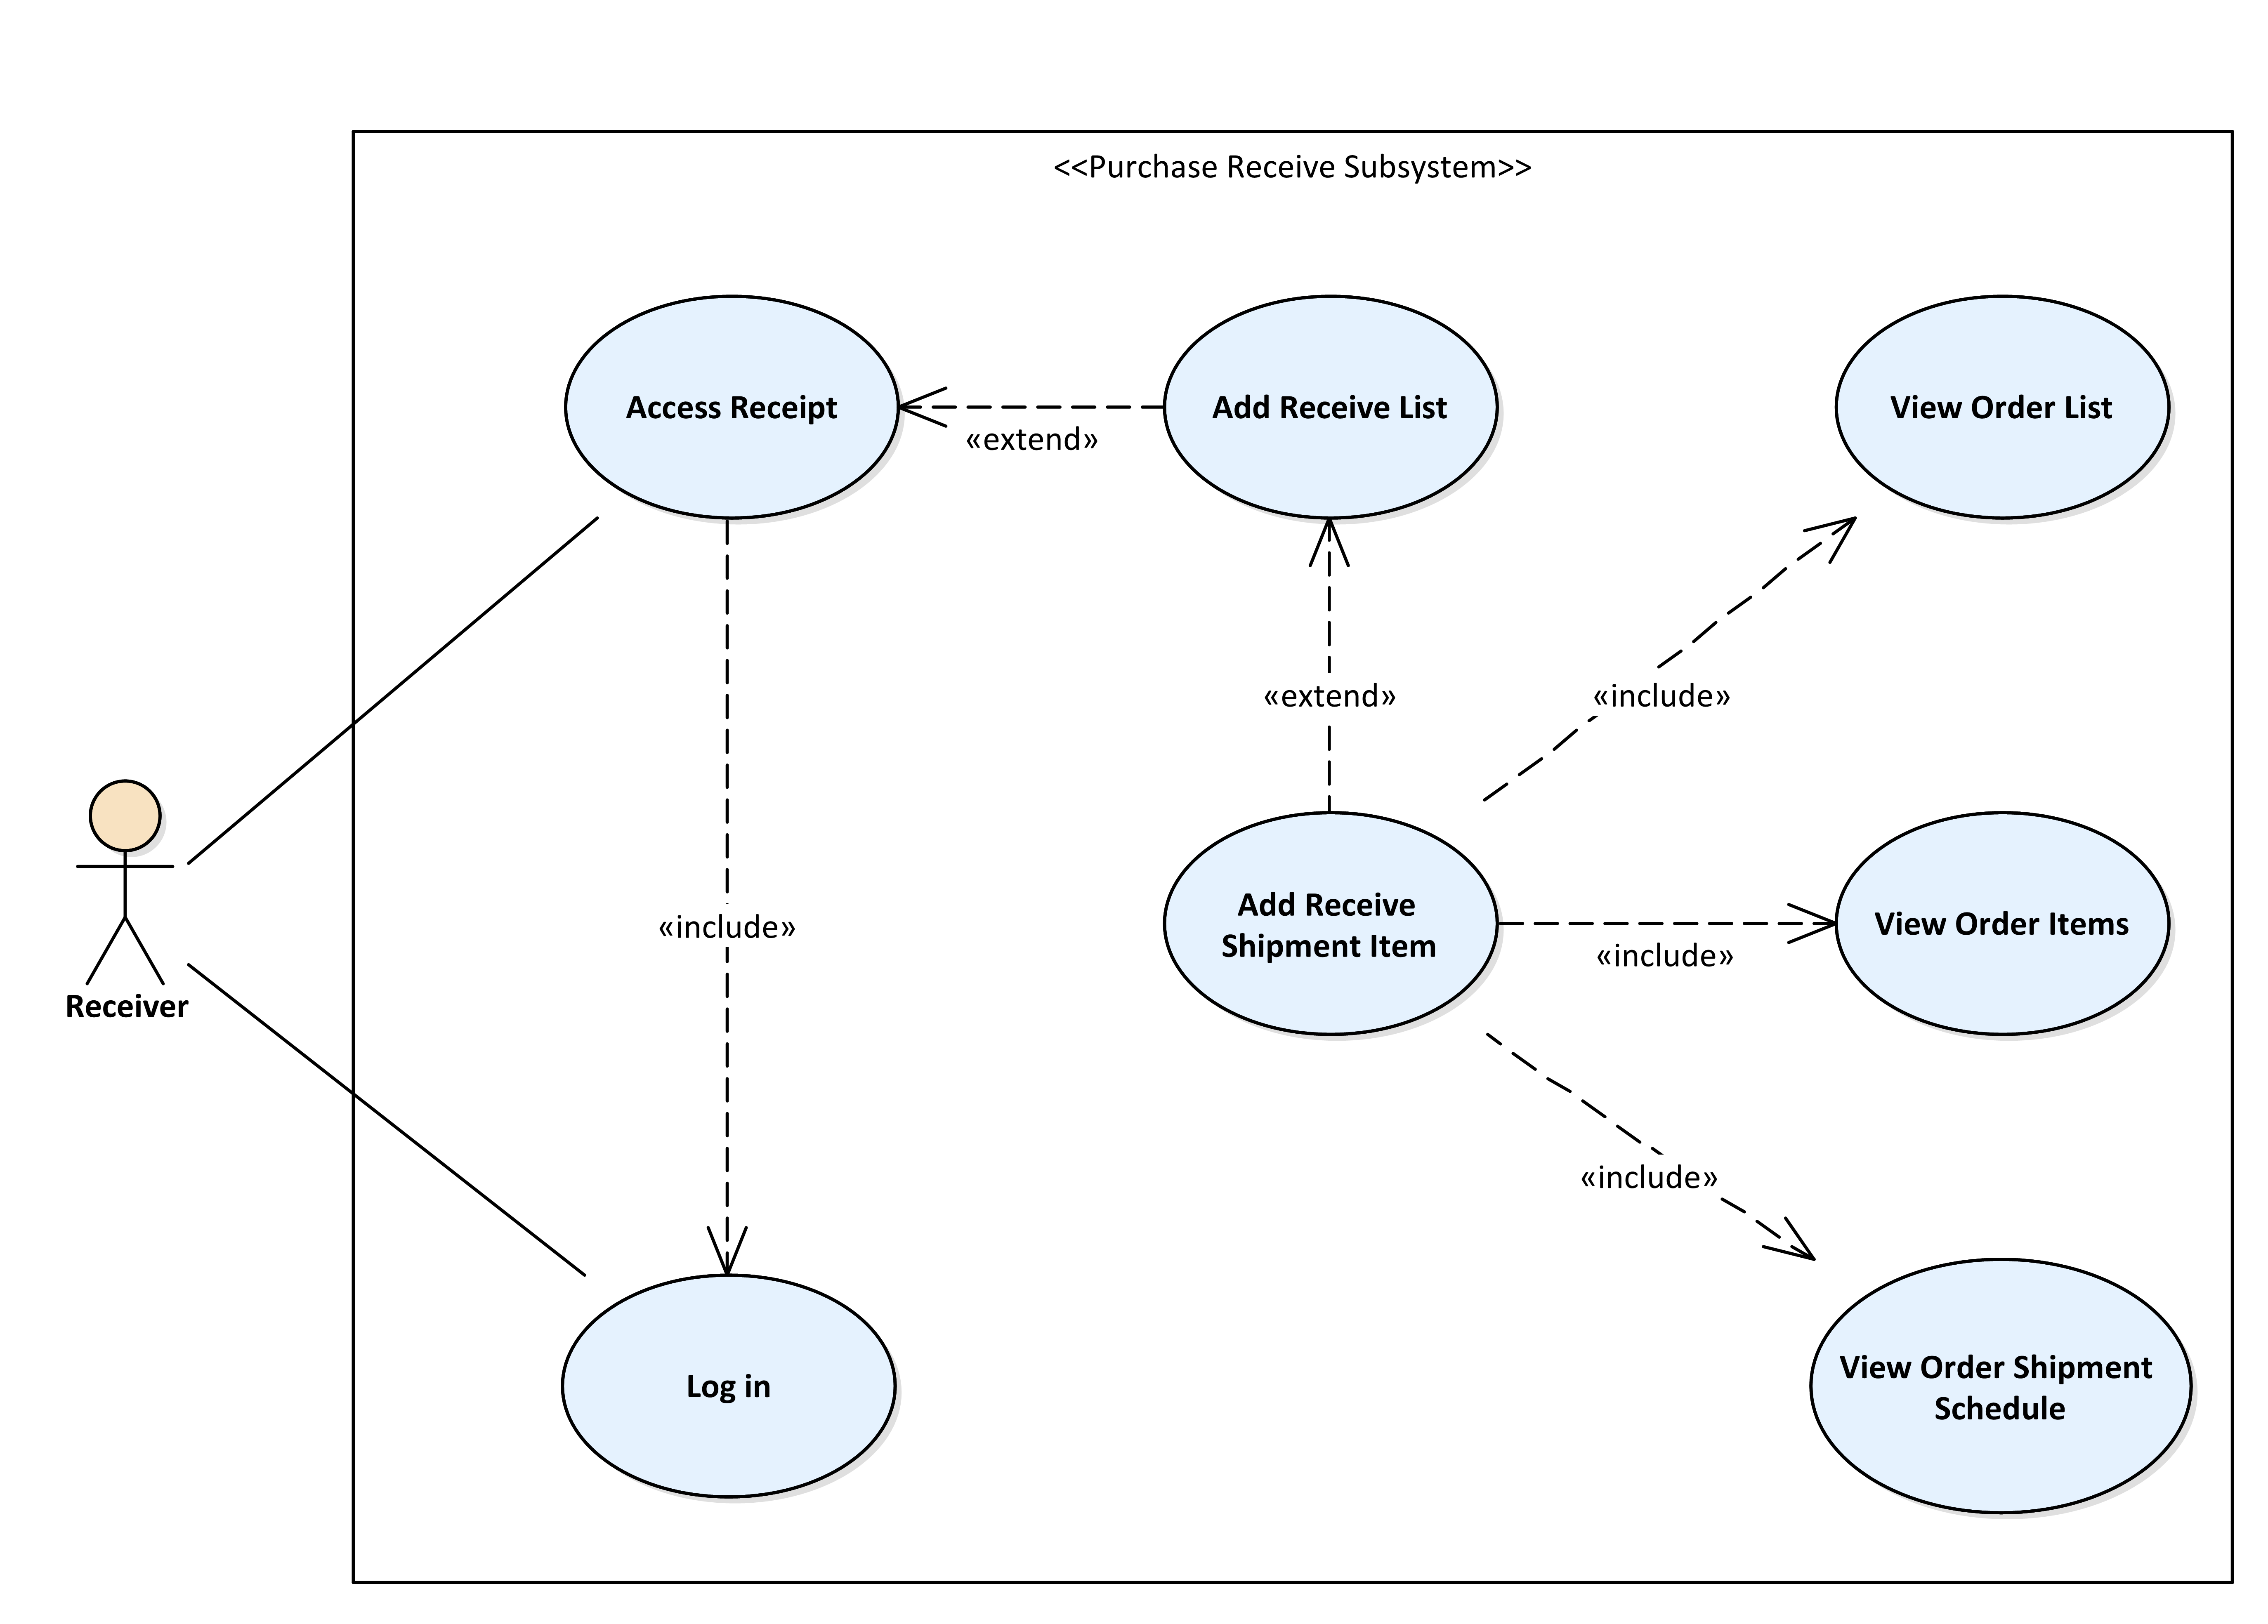
\includegraphics[width=.8\textwidth]{pic/usecase/seupr_usecase_receiver.png}
	\caption{Purchase Receive Use-case Diagram}
	\label{fig:seupr_usecase_receiver}
\end{figure}
%\clearpage


\begin{table}
\begin{tabular}{|l|l|}
\hline
 Name & Purchase Receive \\
\hline
 ID & UC-5 \\
 \hline
 Description & 
 \vtop{
 		\hbox{\strut Receiver wants to access the receipt list and add new receipt list}				
 		\hbox{\strut Receiver wants to add new receipt item}

	}\\
\hline
 Primary Actor & Receiver \\
 \hline
 Secondary Actor & None \\
\hline
 Preconditions & Receiver must log-in the system and have the required roles\\
 \hline
 Postconditions & System generates new receive list and items \\
\hline
 Main Flow &  
		
	\vtop{
 		\hbox{\strut Receiver log-in the system}	
 		\hbox{\strut Receiver access receive list}
 		\hbox{\strut Receiver creates new receive list}
 		\hbox{\strut Receiver creates new receive items}
 		\hbox{\strut Receiver views requisition item shipment schedules}	

 		\hbox{\strut Usecase ends}			 								
	}\\		
 \hline
\end{tabular}
\end{table}

% all usecase commenting================
% all usecase commenting================

\fi

\clearpage









\newgeometry{bottom=1cm,left=1cm, top=0cm, right=0cm}
\begin{landscape}
\subsection{Activity Diagram}
\begin{figure}[h]
%Activity diagrams combination of activities for a system and represents the flow of use cases and work-flows of step-wise activities and actions. The activity is described as operation in the system. Activity diagram can show that are conditional or parallel. \\

	\begin{center}
	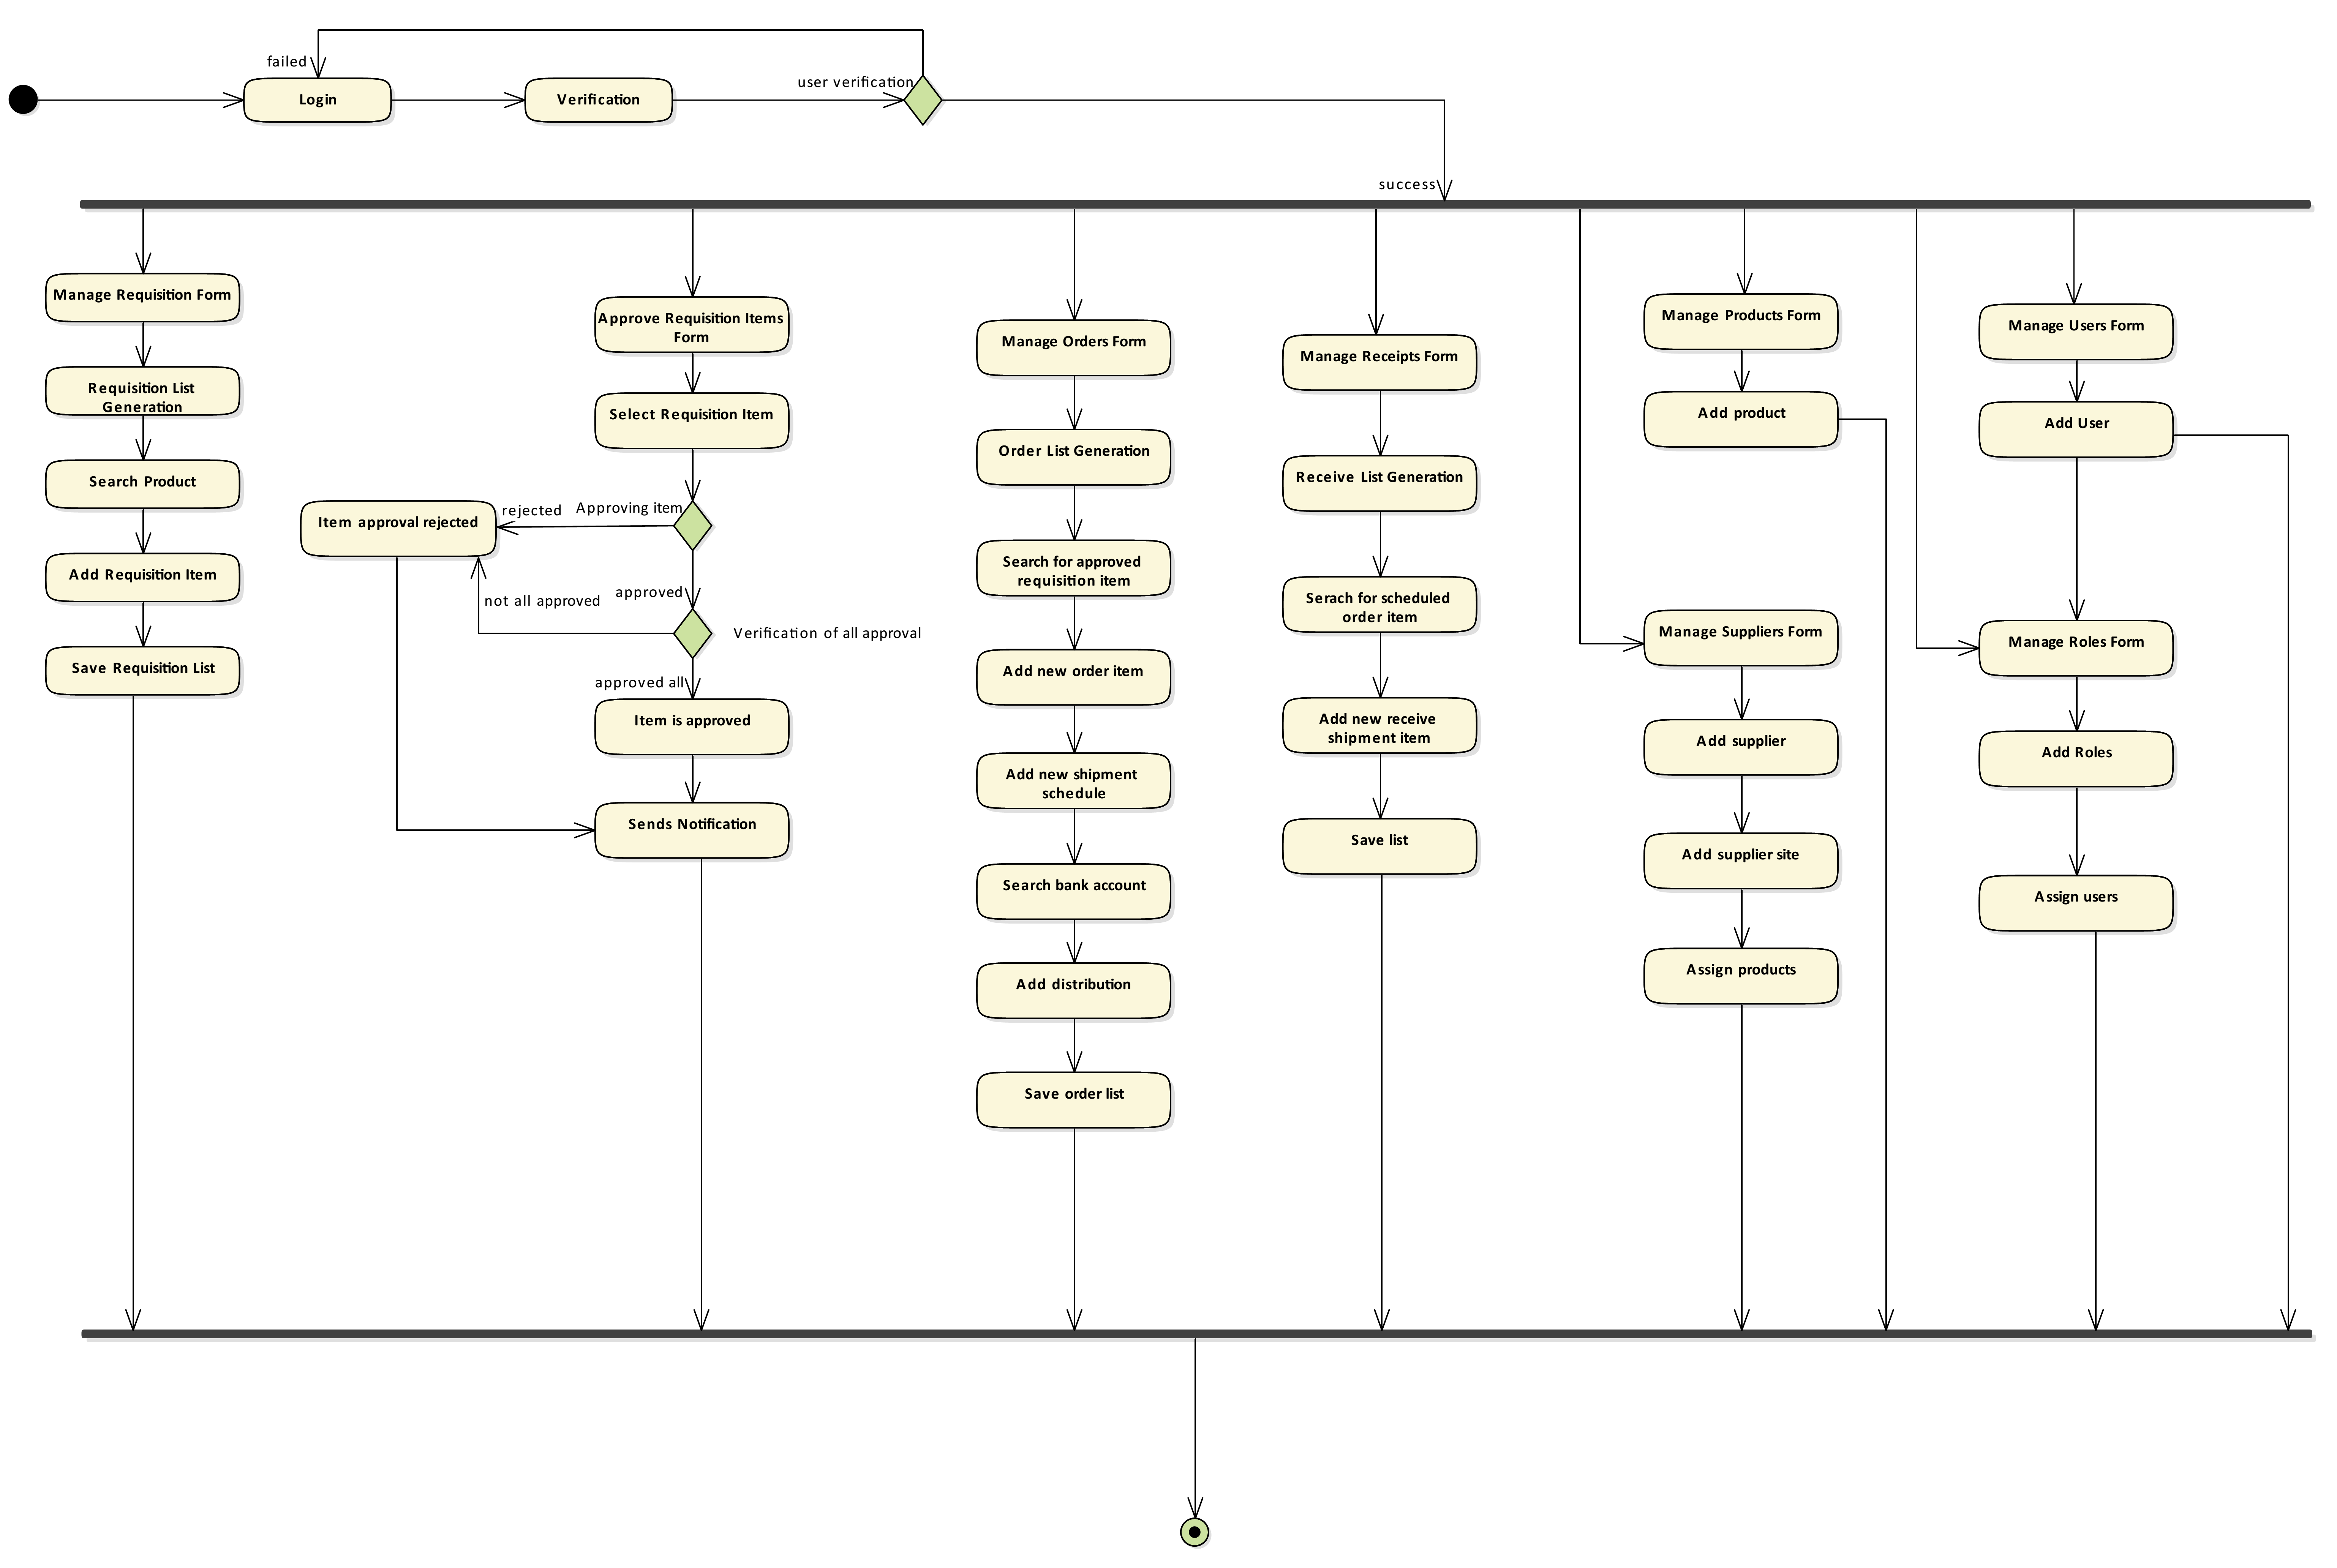
\includegraphics[width=1\textwidth]{pic/Activity/seupr_full_activity.png}
	\end{center}
	\caption{SEU Purchase Requisition Activity Diagram}
	\label{fig:activity}
\end{figure}
%\clearpage
\thispagestyle{empty} 
\end{landscape}
%\clearpage

\restoregeometry




% all Activity commenting================
% all Activity commenting================

\ifx

\begin{figure}[h]
	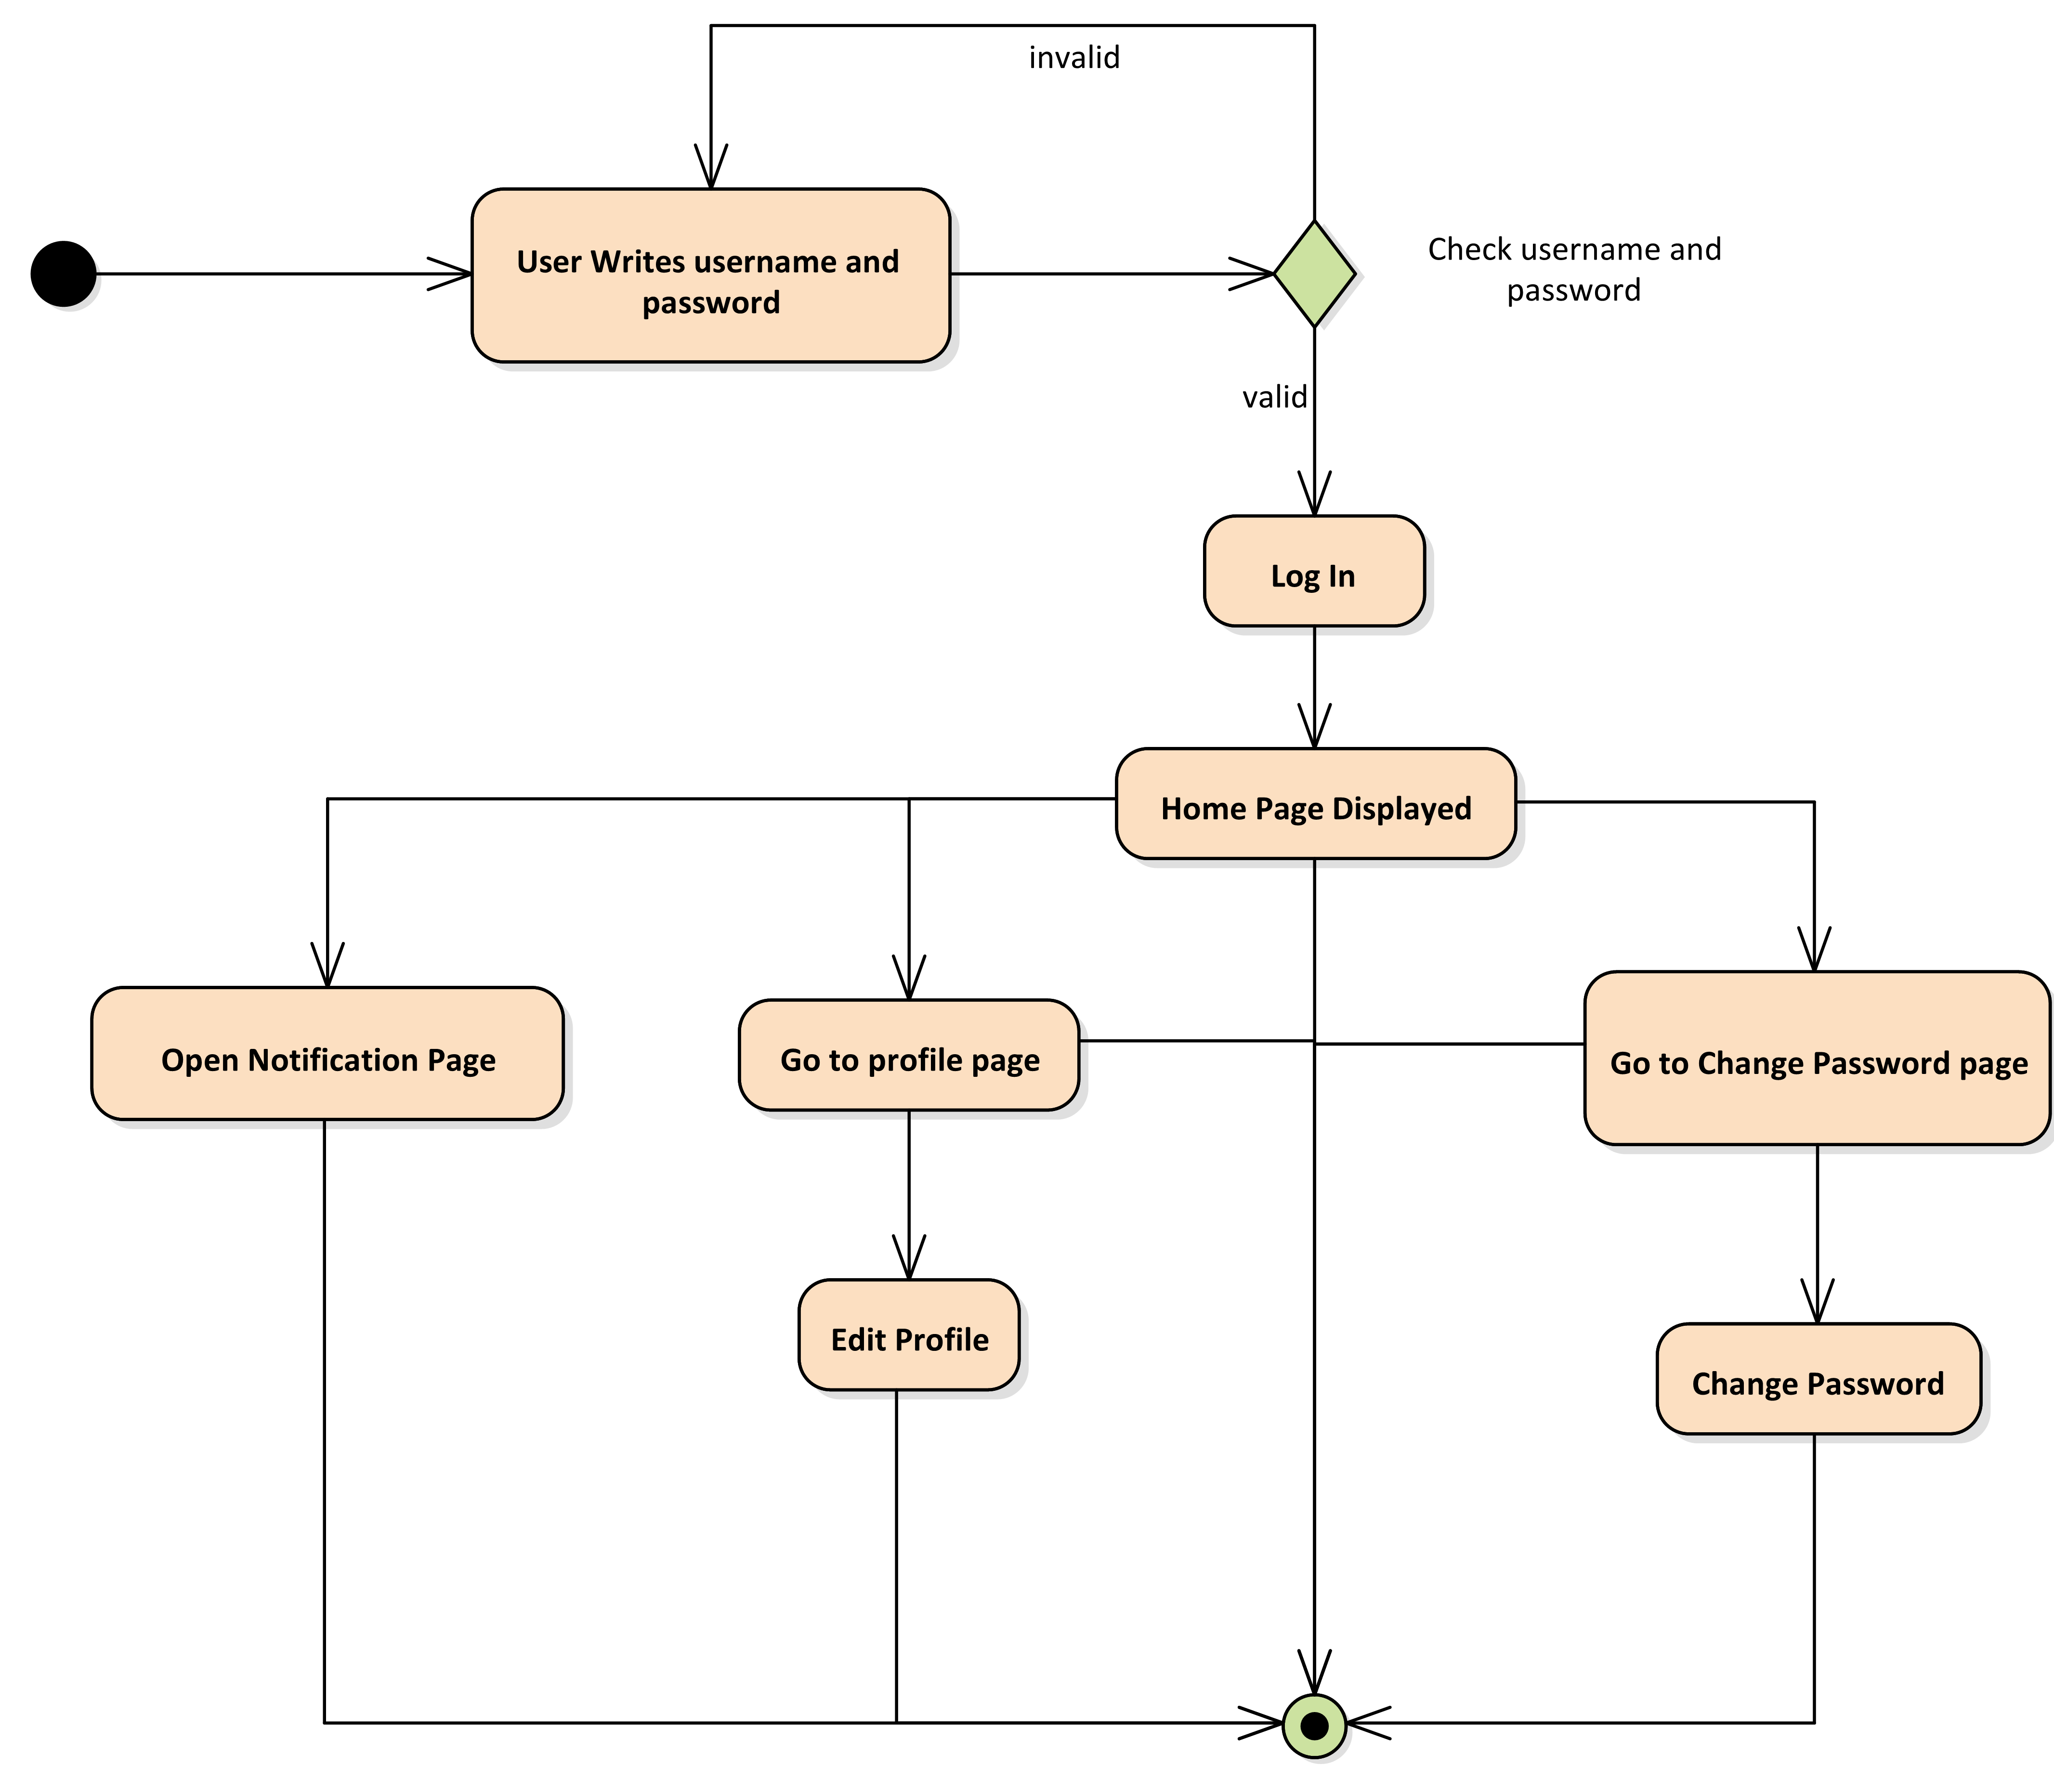
\includegraphics[width=1\textwidth]{pic/Activity/login.png}
	\caption{log-in Activity Diagram}
	\label{fig:login}
\end{figure}


\begin{figure}[h]
	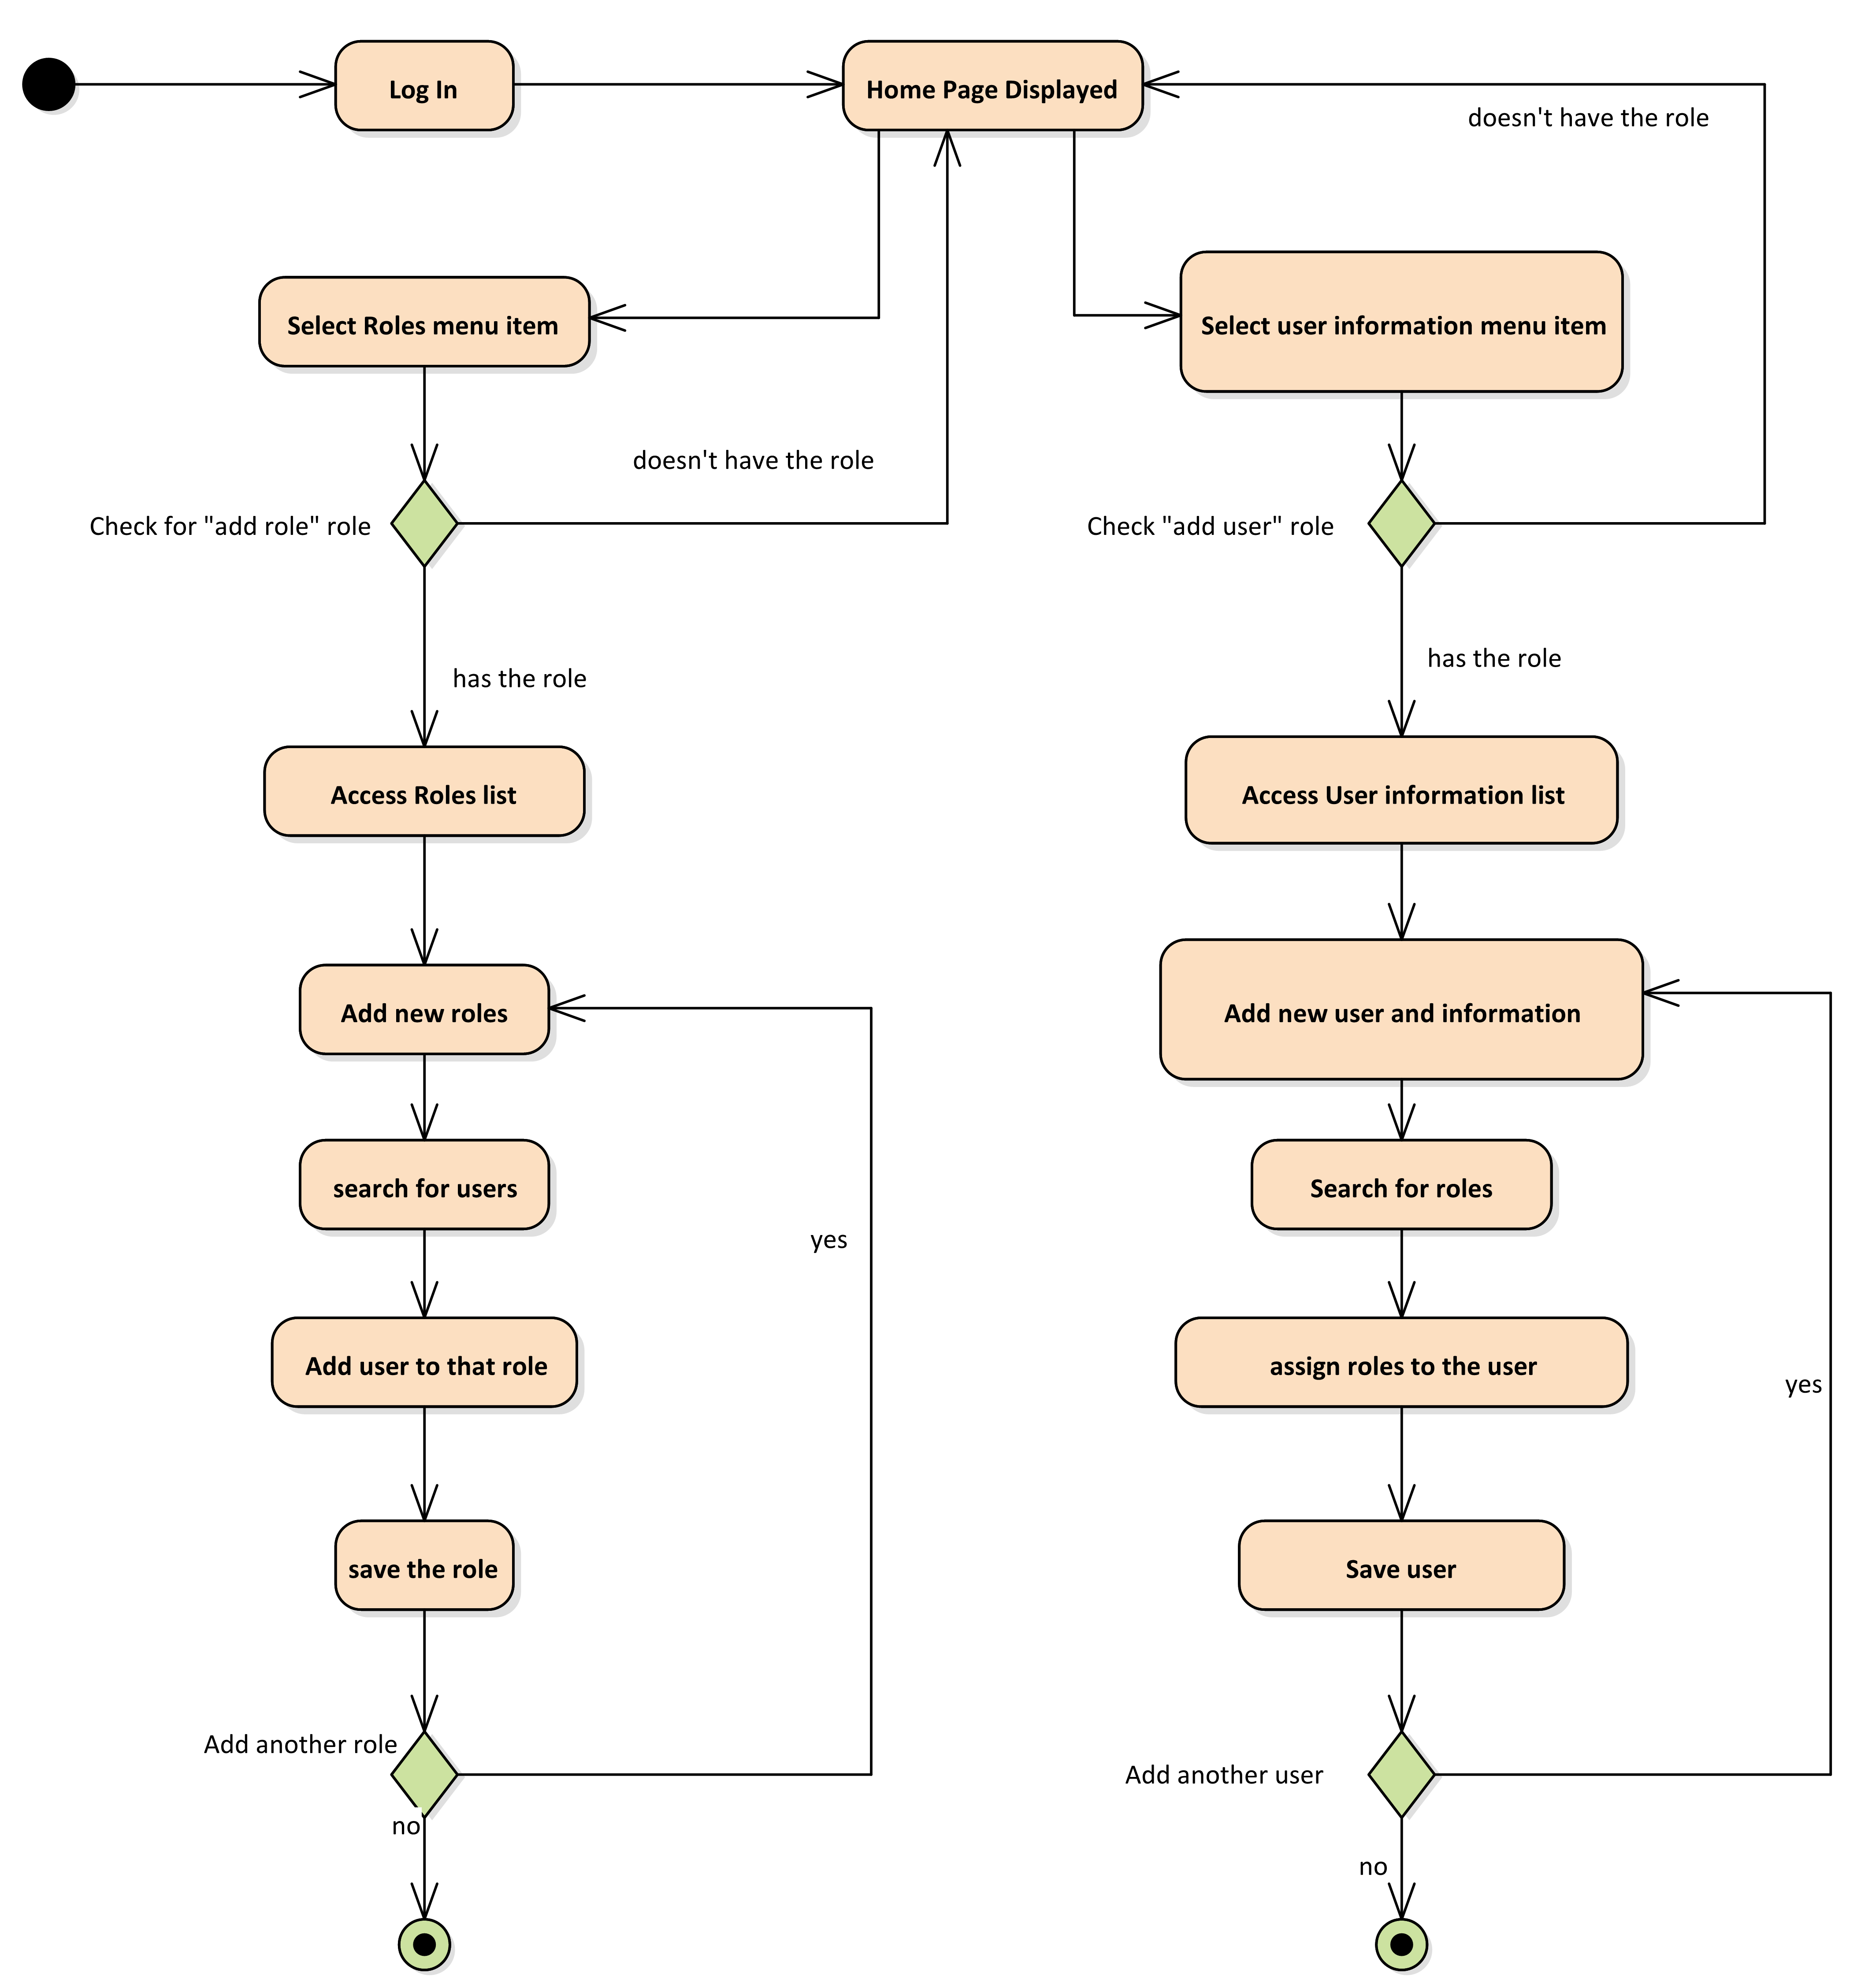
\includegraphics[width=1\textwidth]{pic/Activity/administration.png}
	\caption{Administrating Activity Diagram}
	\label{fig:administration}
\end{figure}



\begin{figure}[h]
	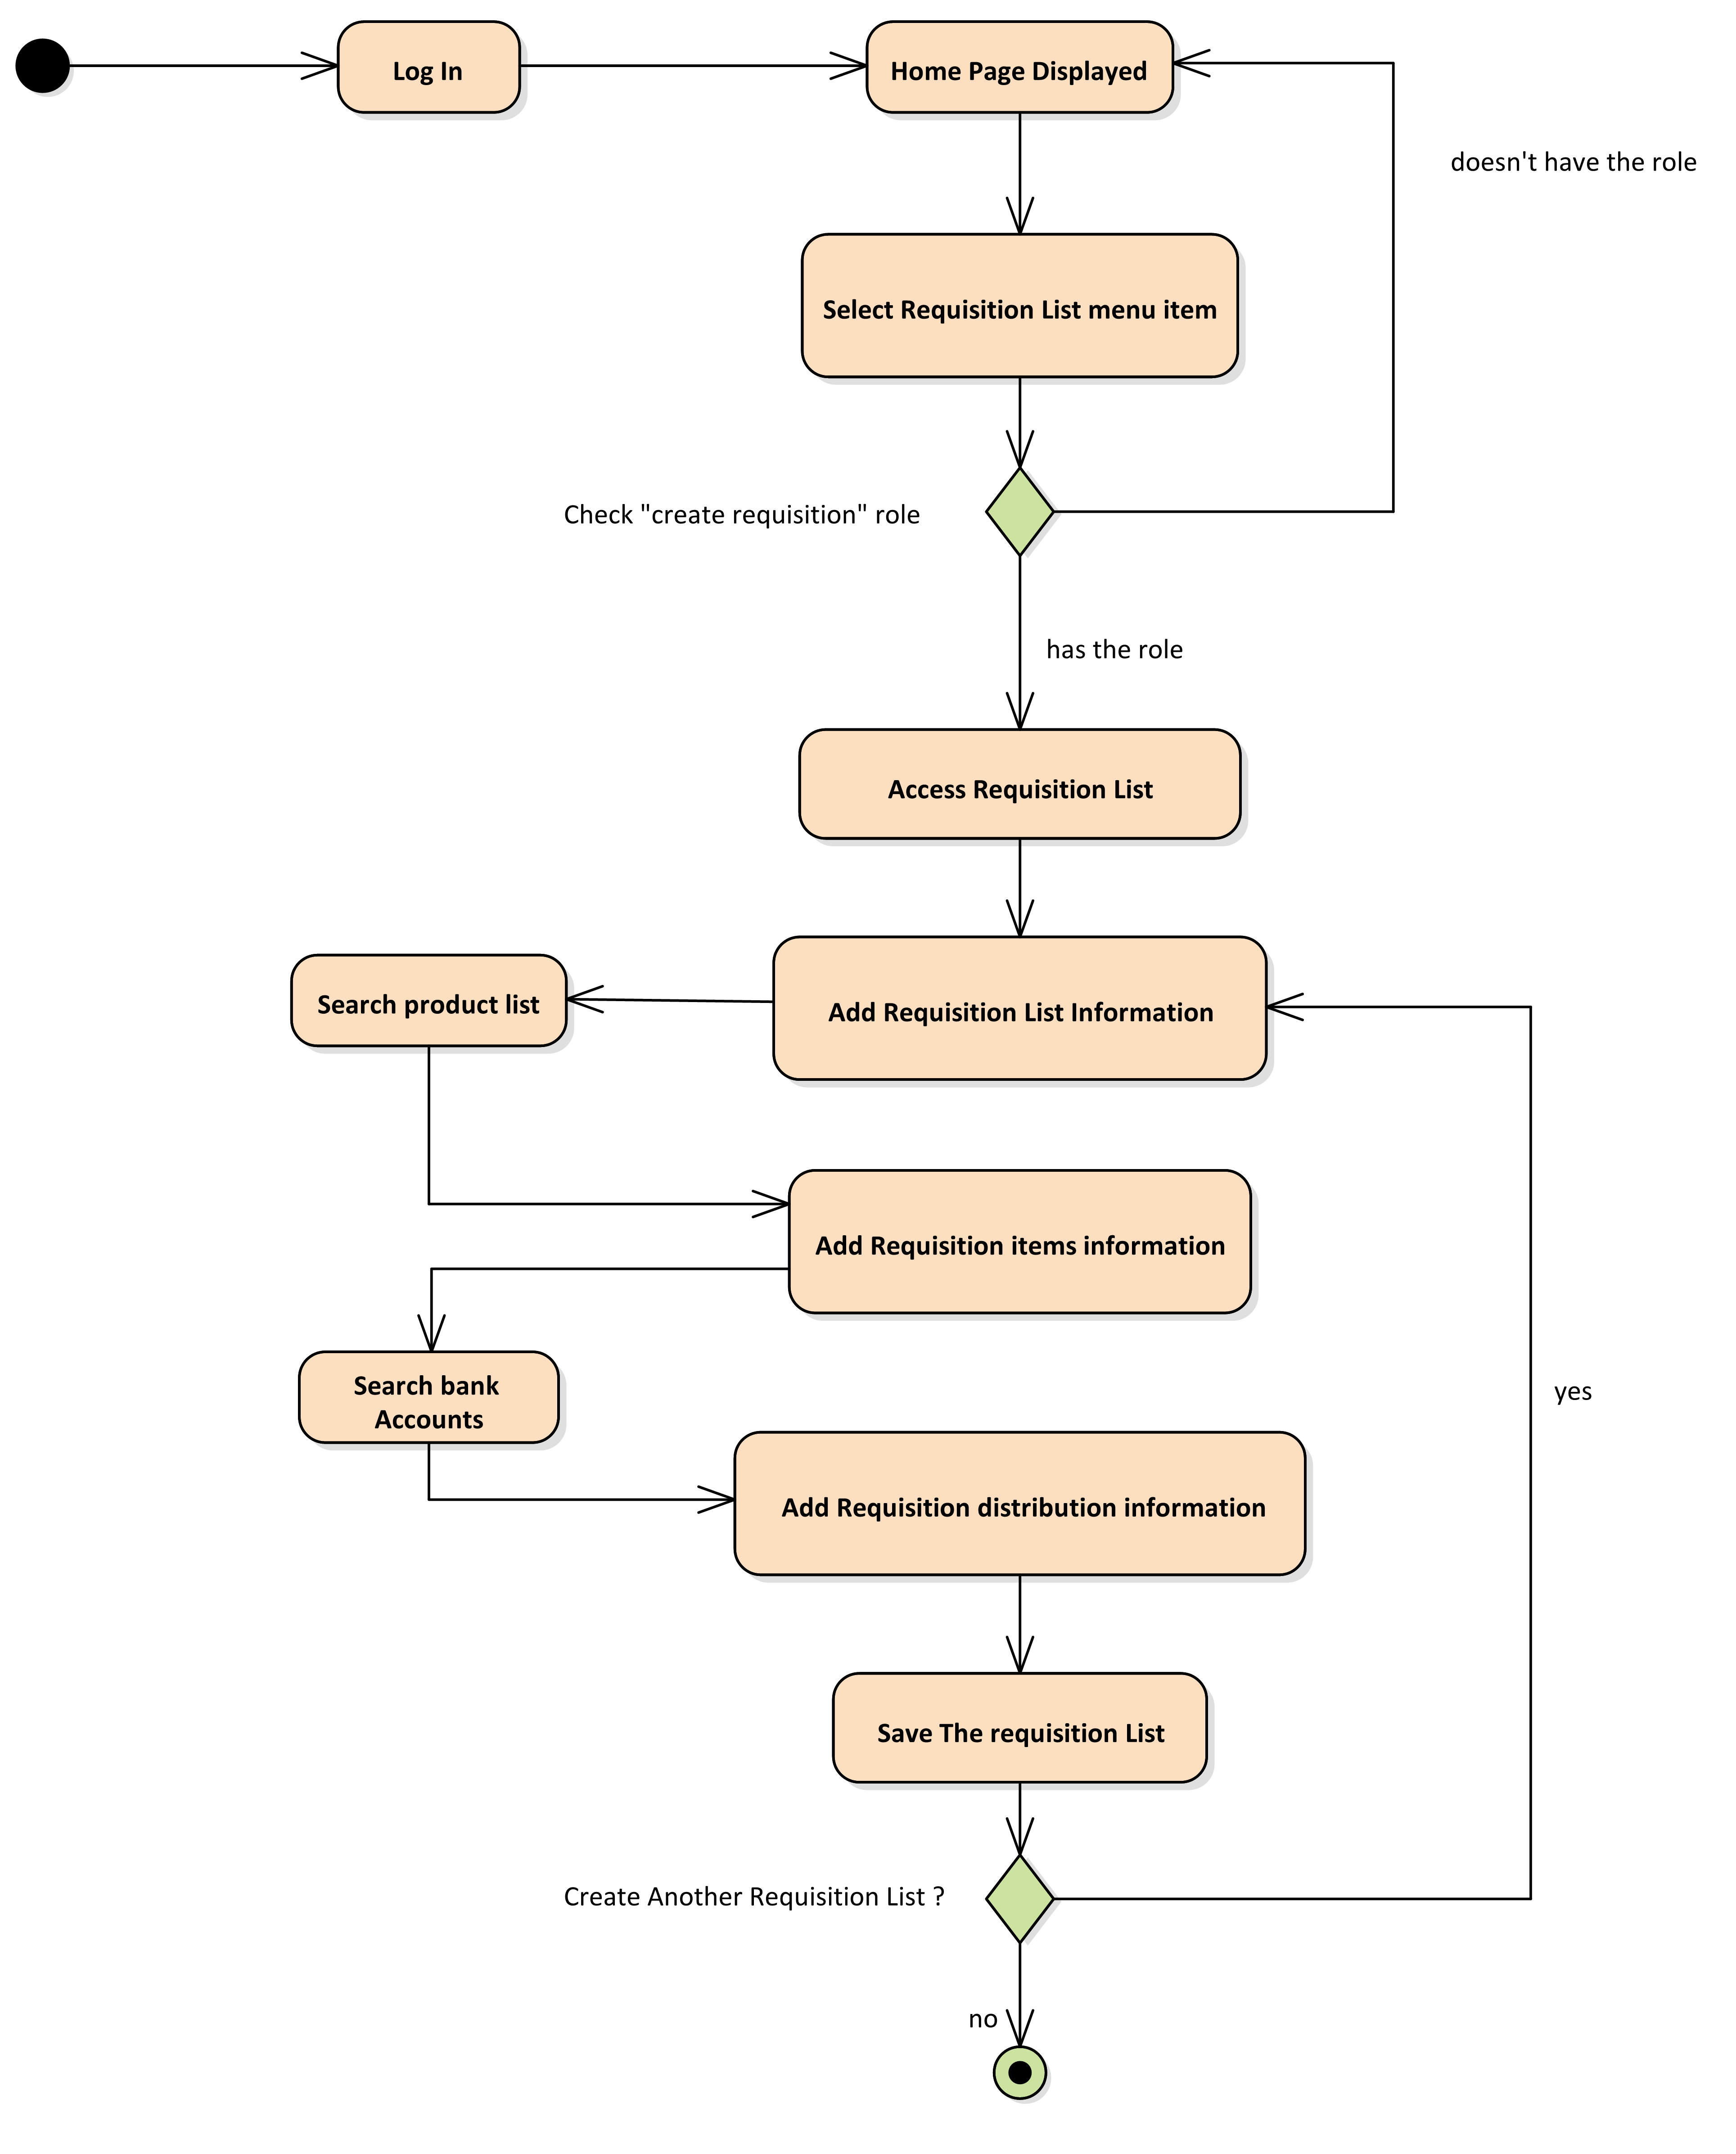
\includegraphics[width=1\textwidth]{pic/Activity/requisition.png}
	\caption{Requisition Activity Diagram}
	\label{fig:requisition}
\end{figure}


\begin{figure}[h]
	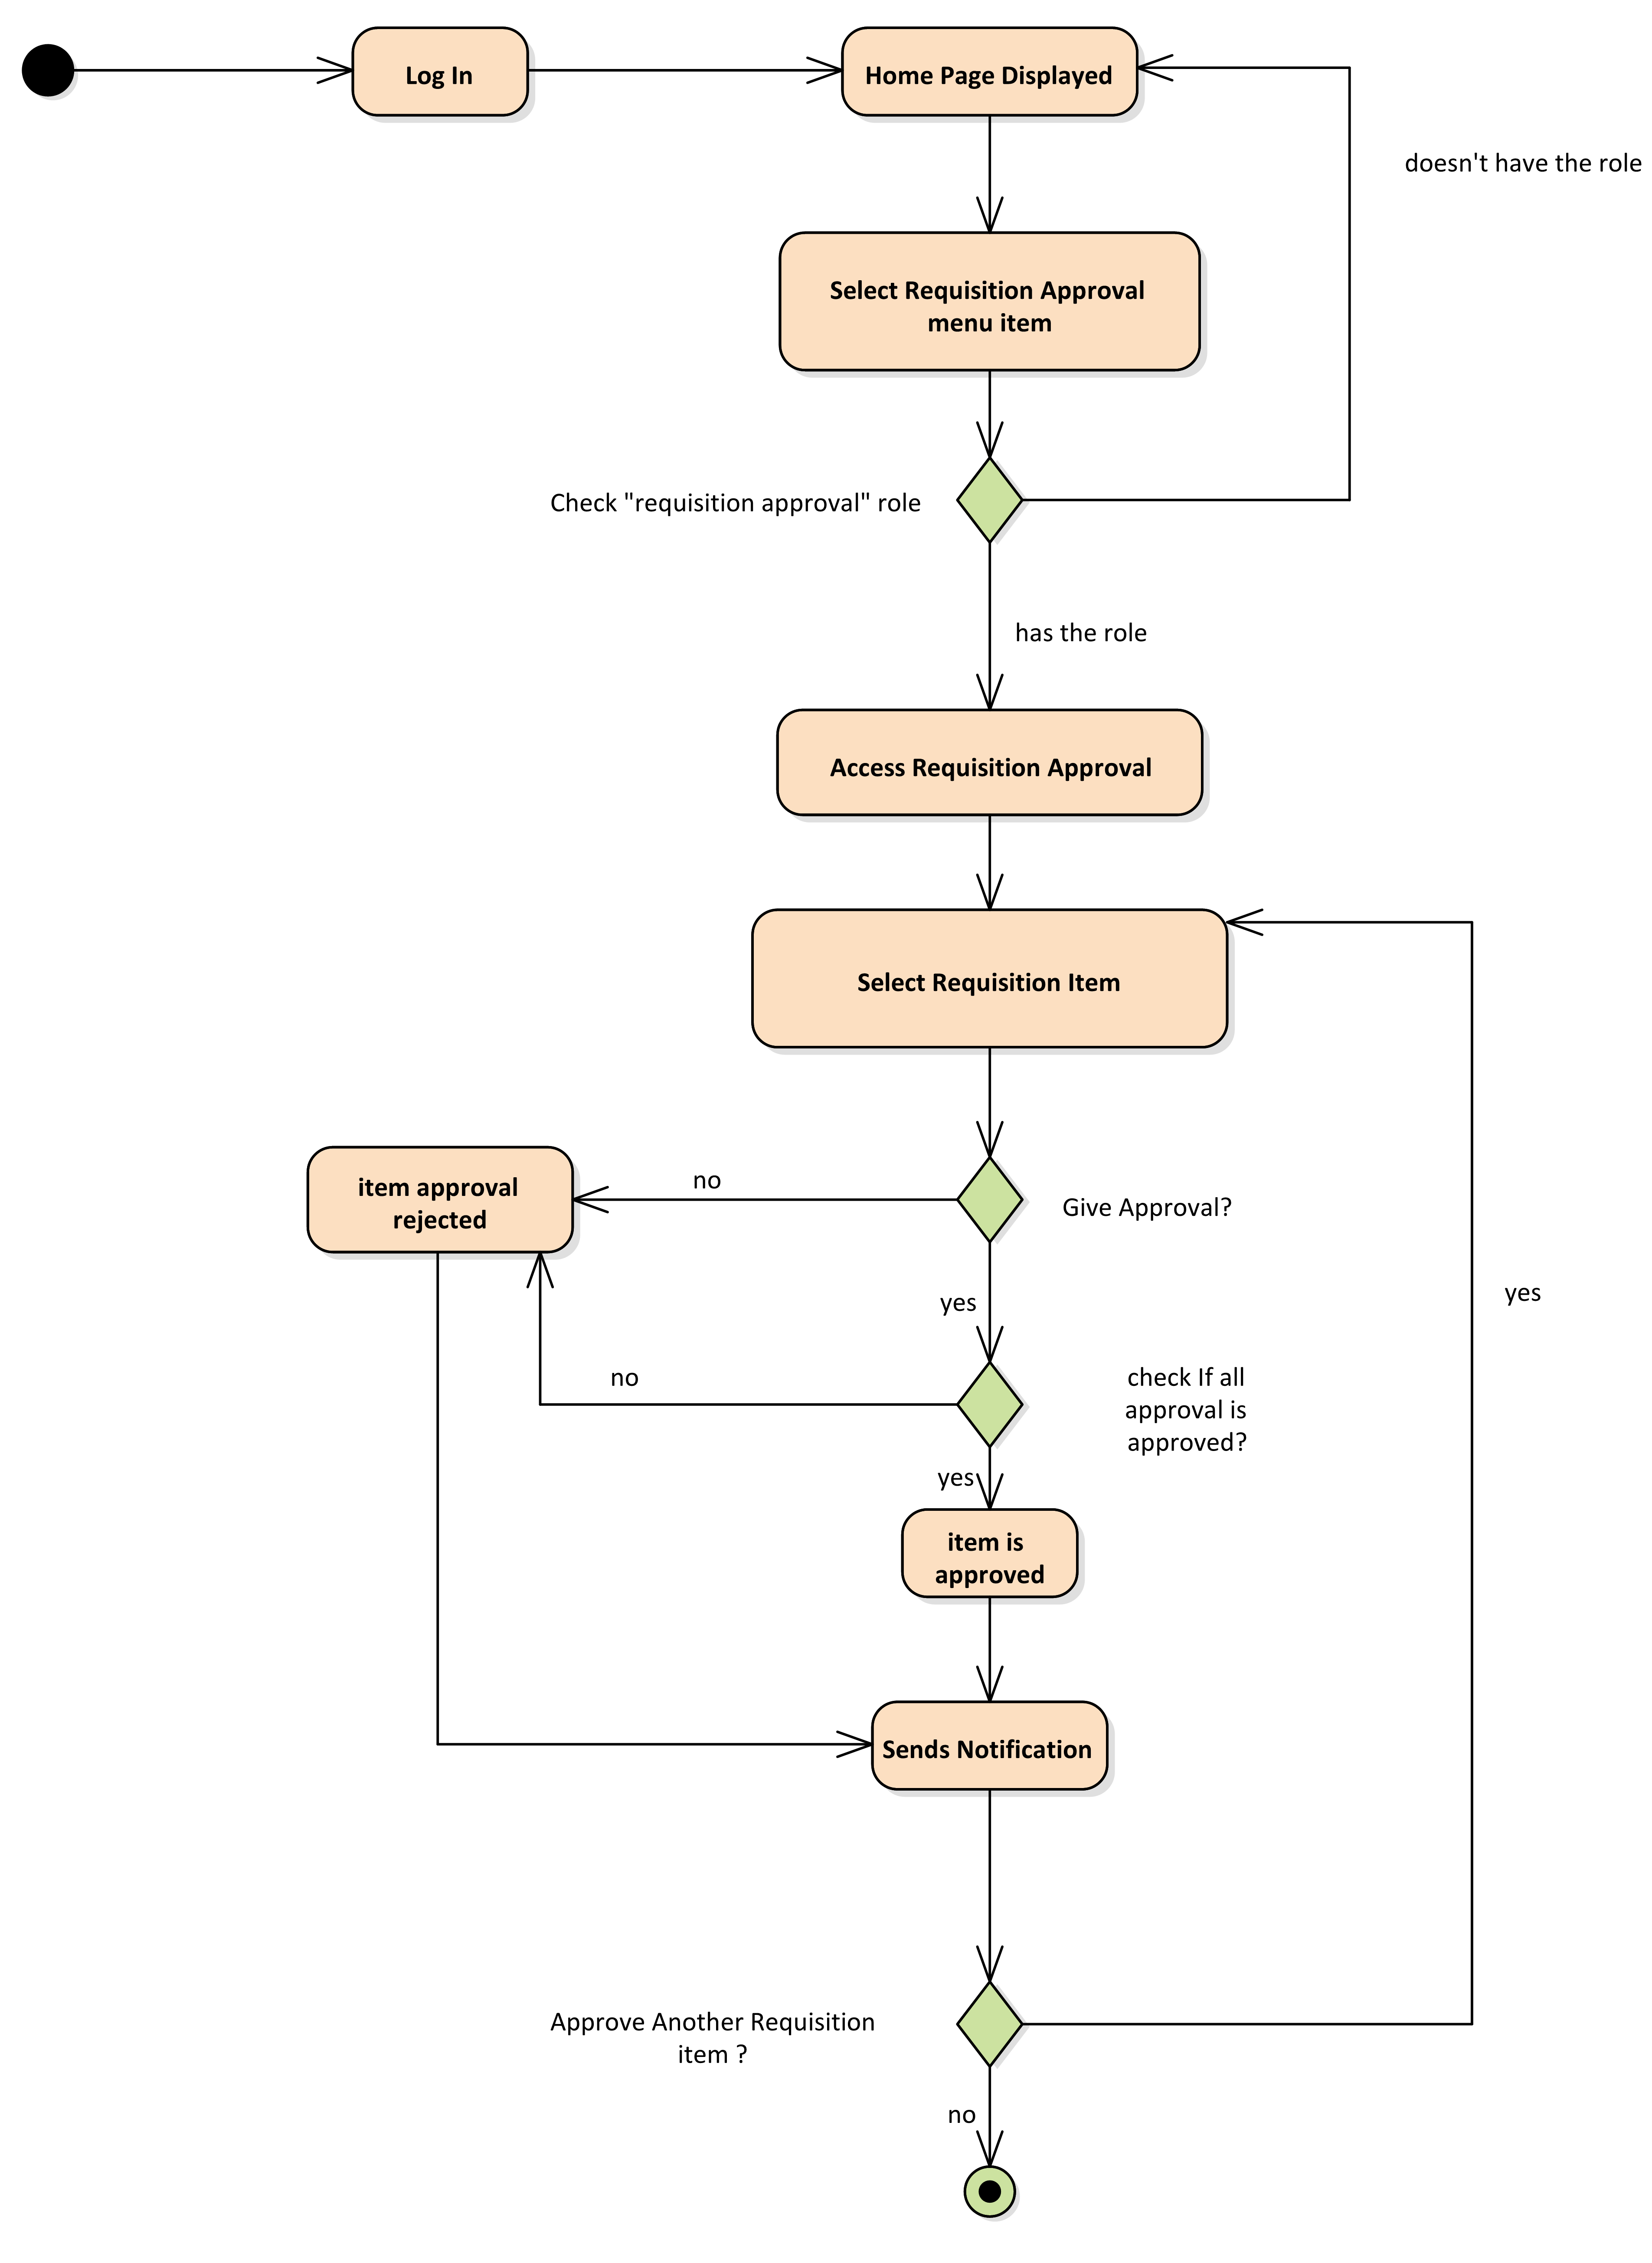
\includegraphics[width=.9\textwidth]{pic/Activity/requisition_approval.png}
	\caption{Requisition Approval Activity Diagram}
	\label{fig:requisition_approval}
\end{figure}


\begin{figure}[h]
	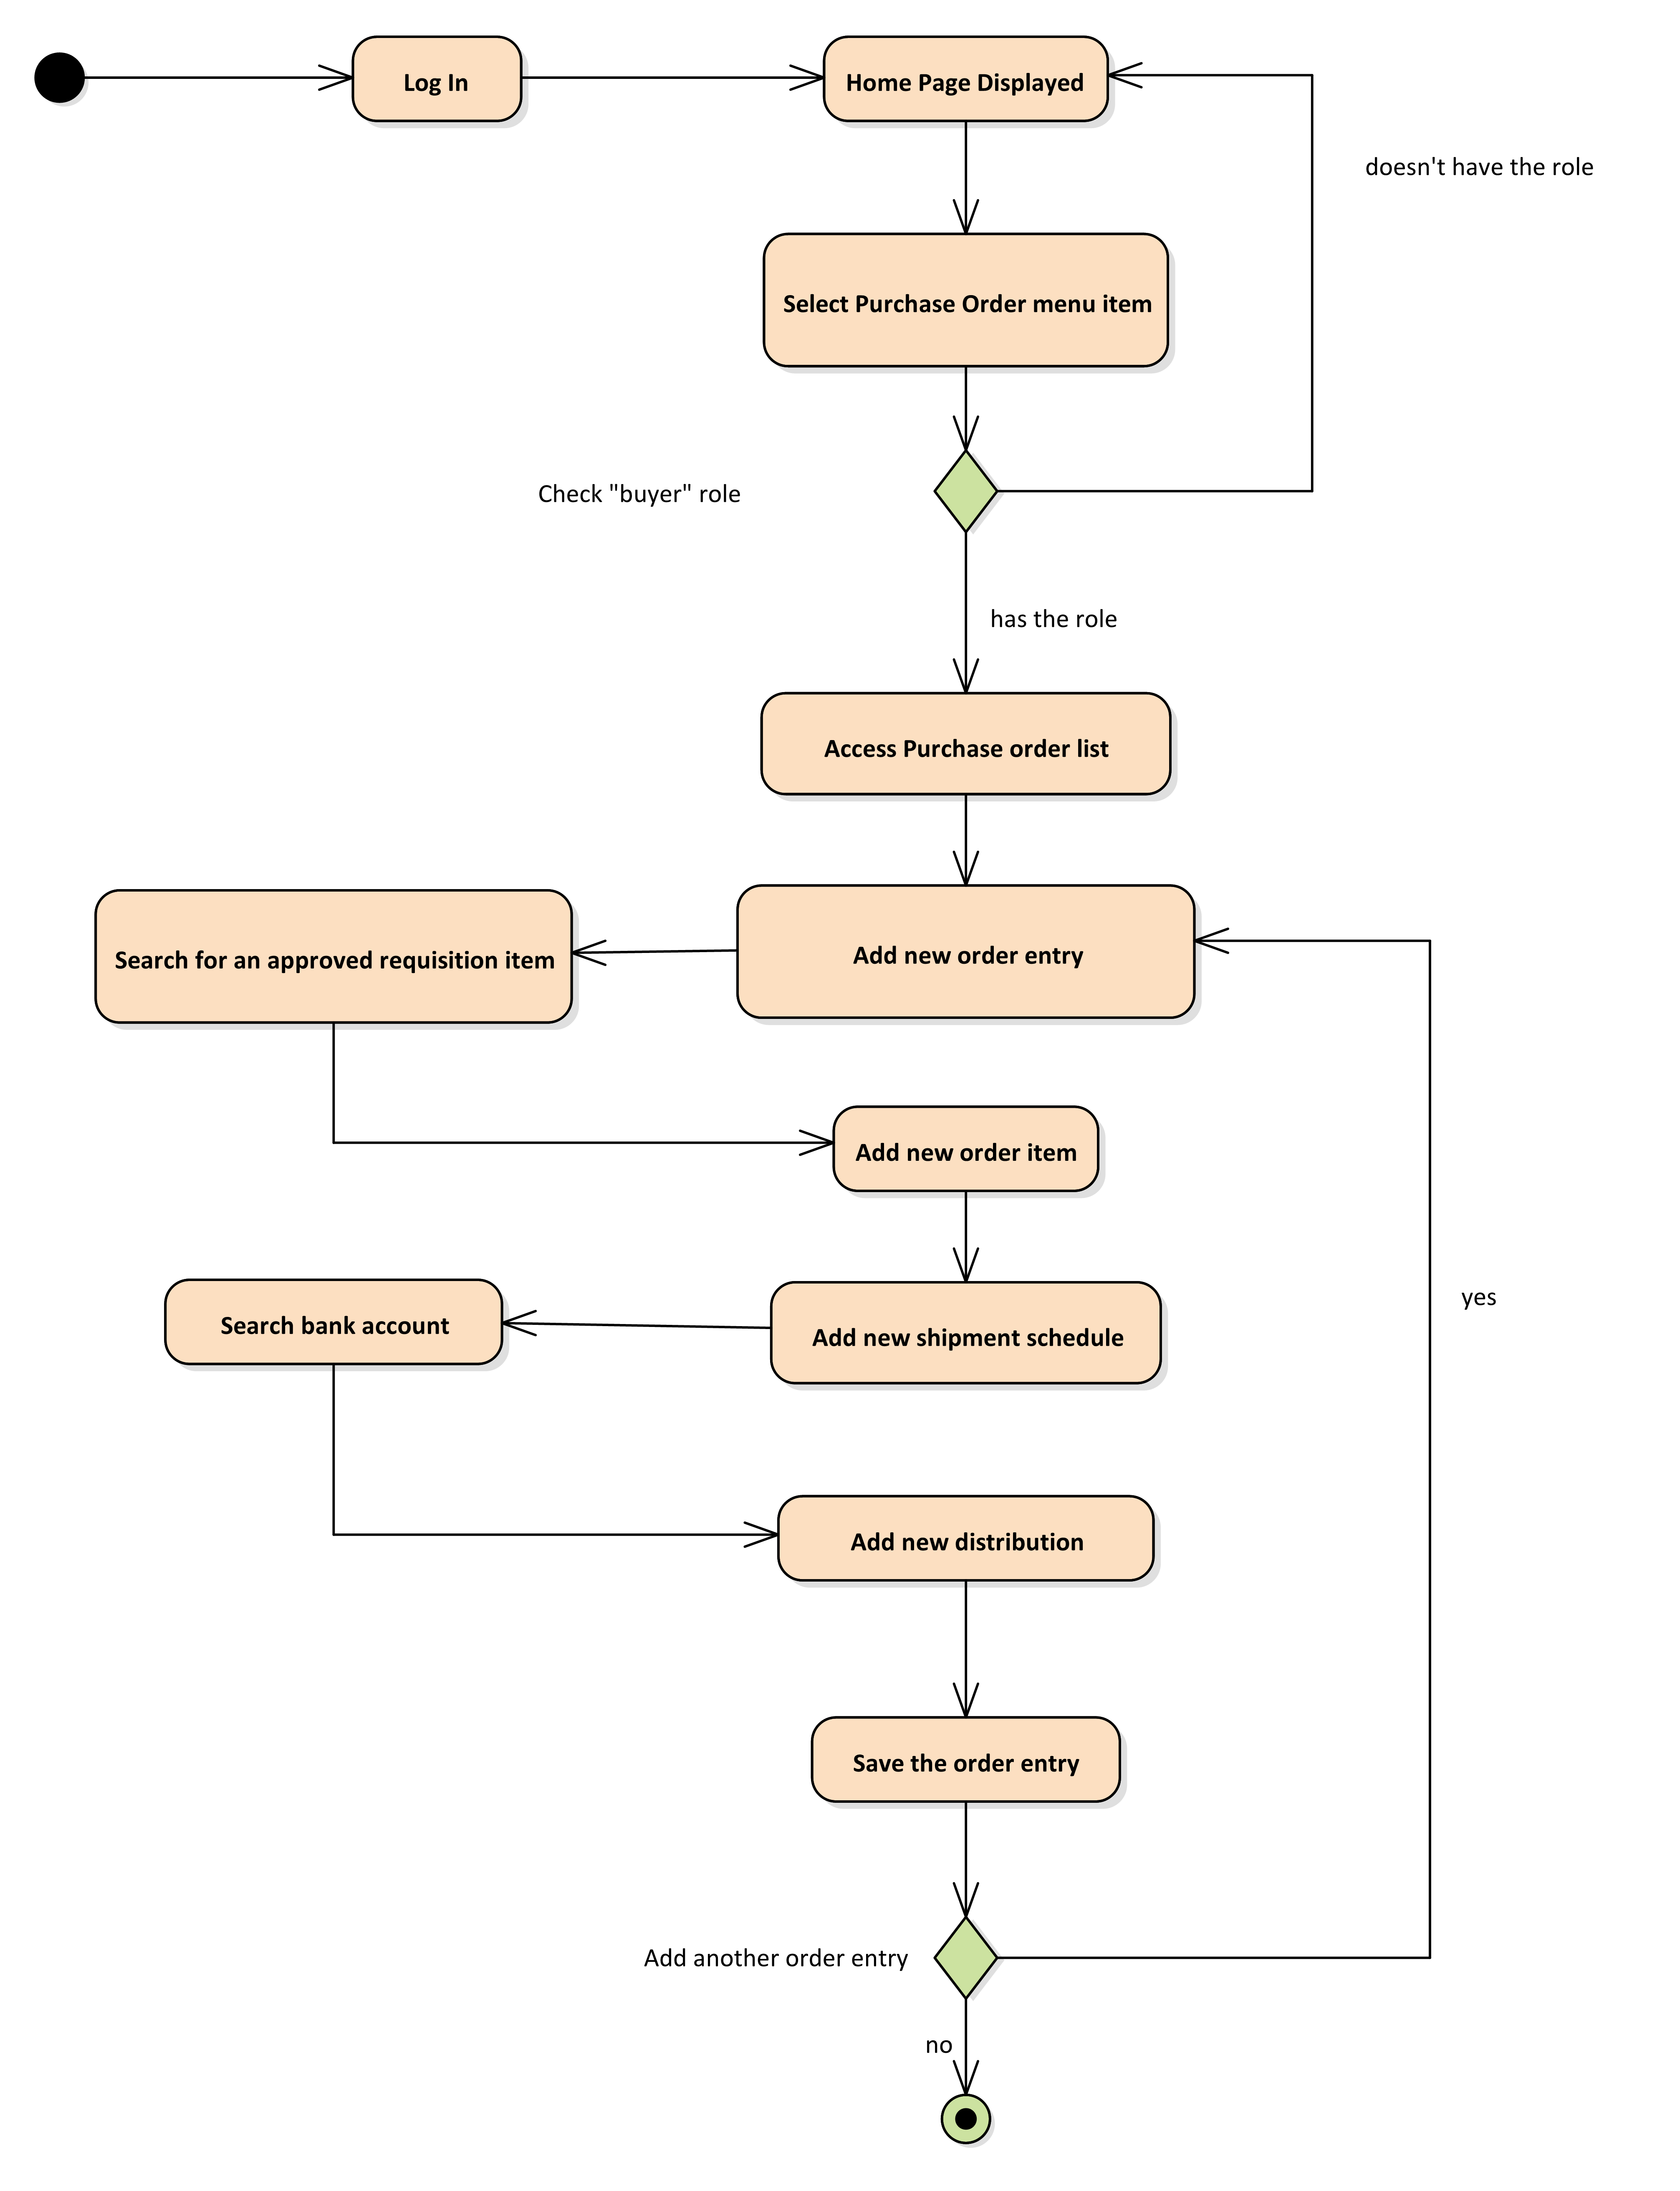
\includegraphics[width=1\textwidth]{pic/Activity/order.png}
	\caption{Order Activity Diagram}
	\label{fig:order}
\end{figure}

\begin{figure}[h]
	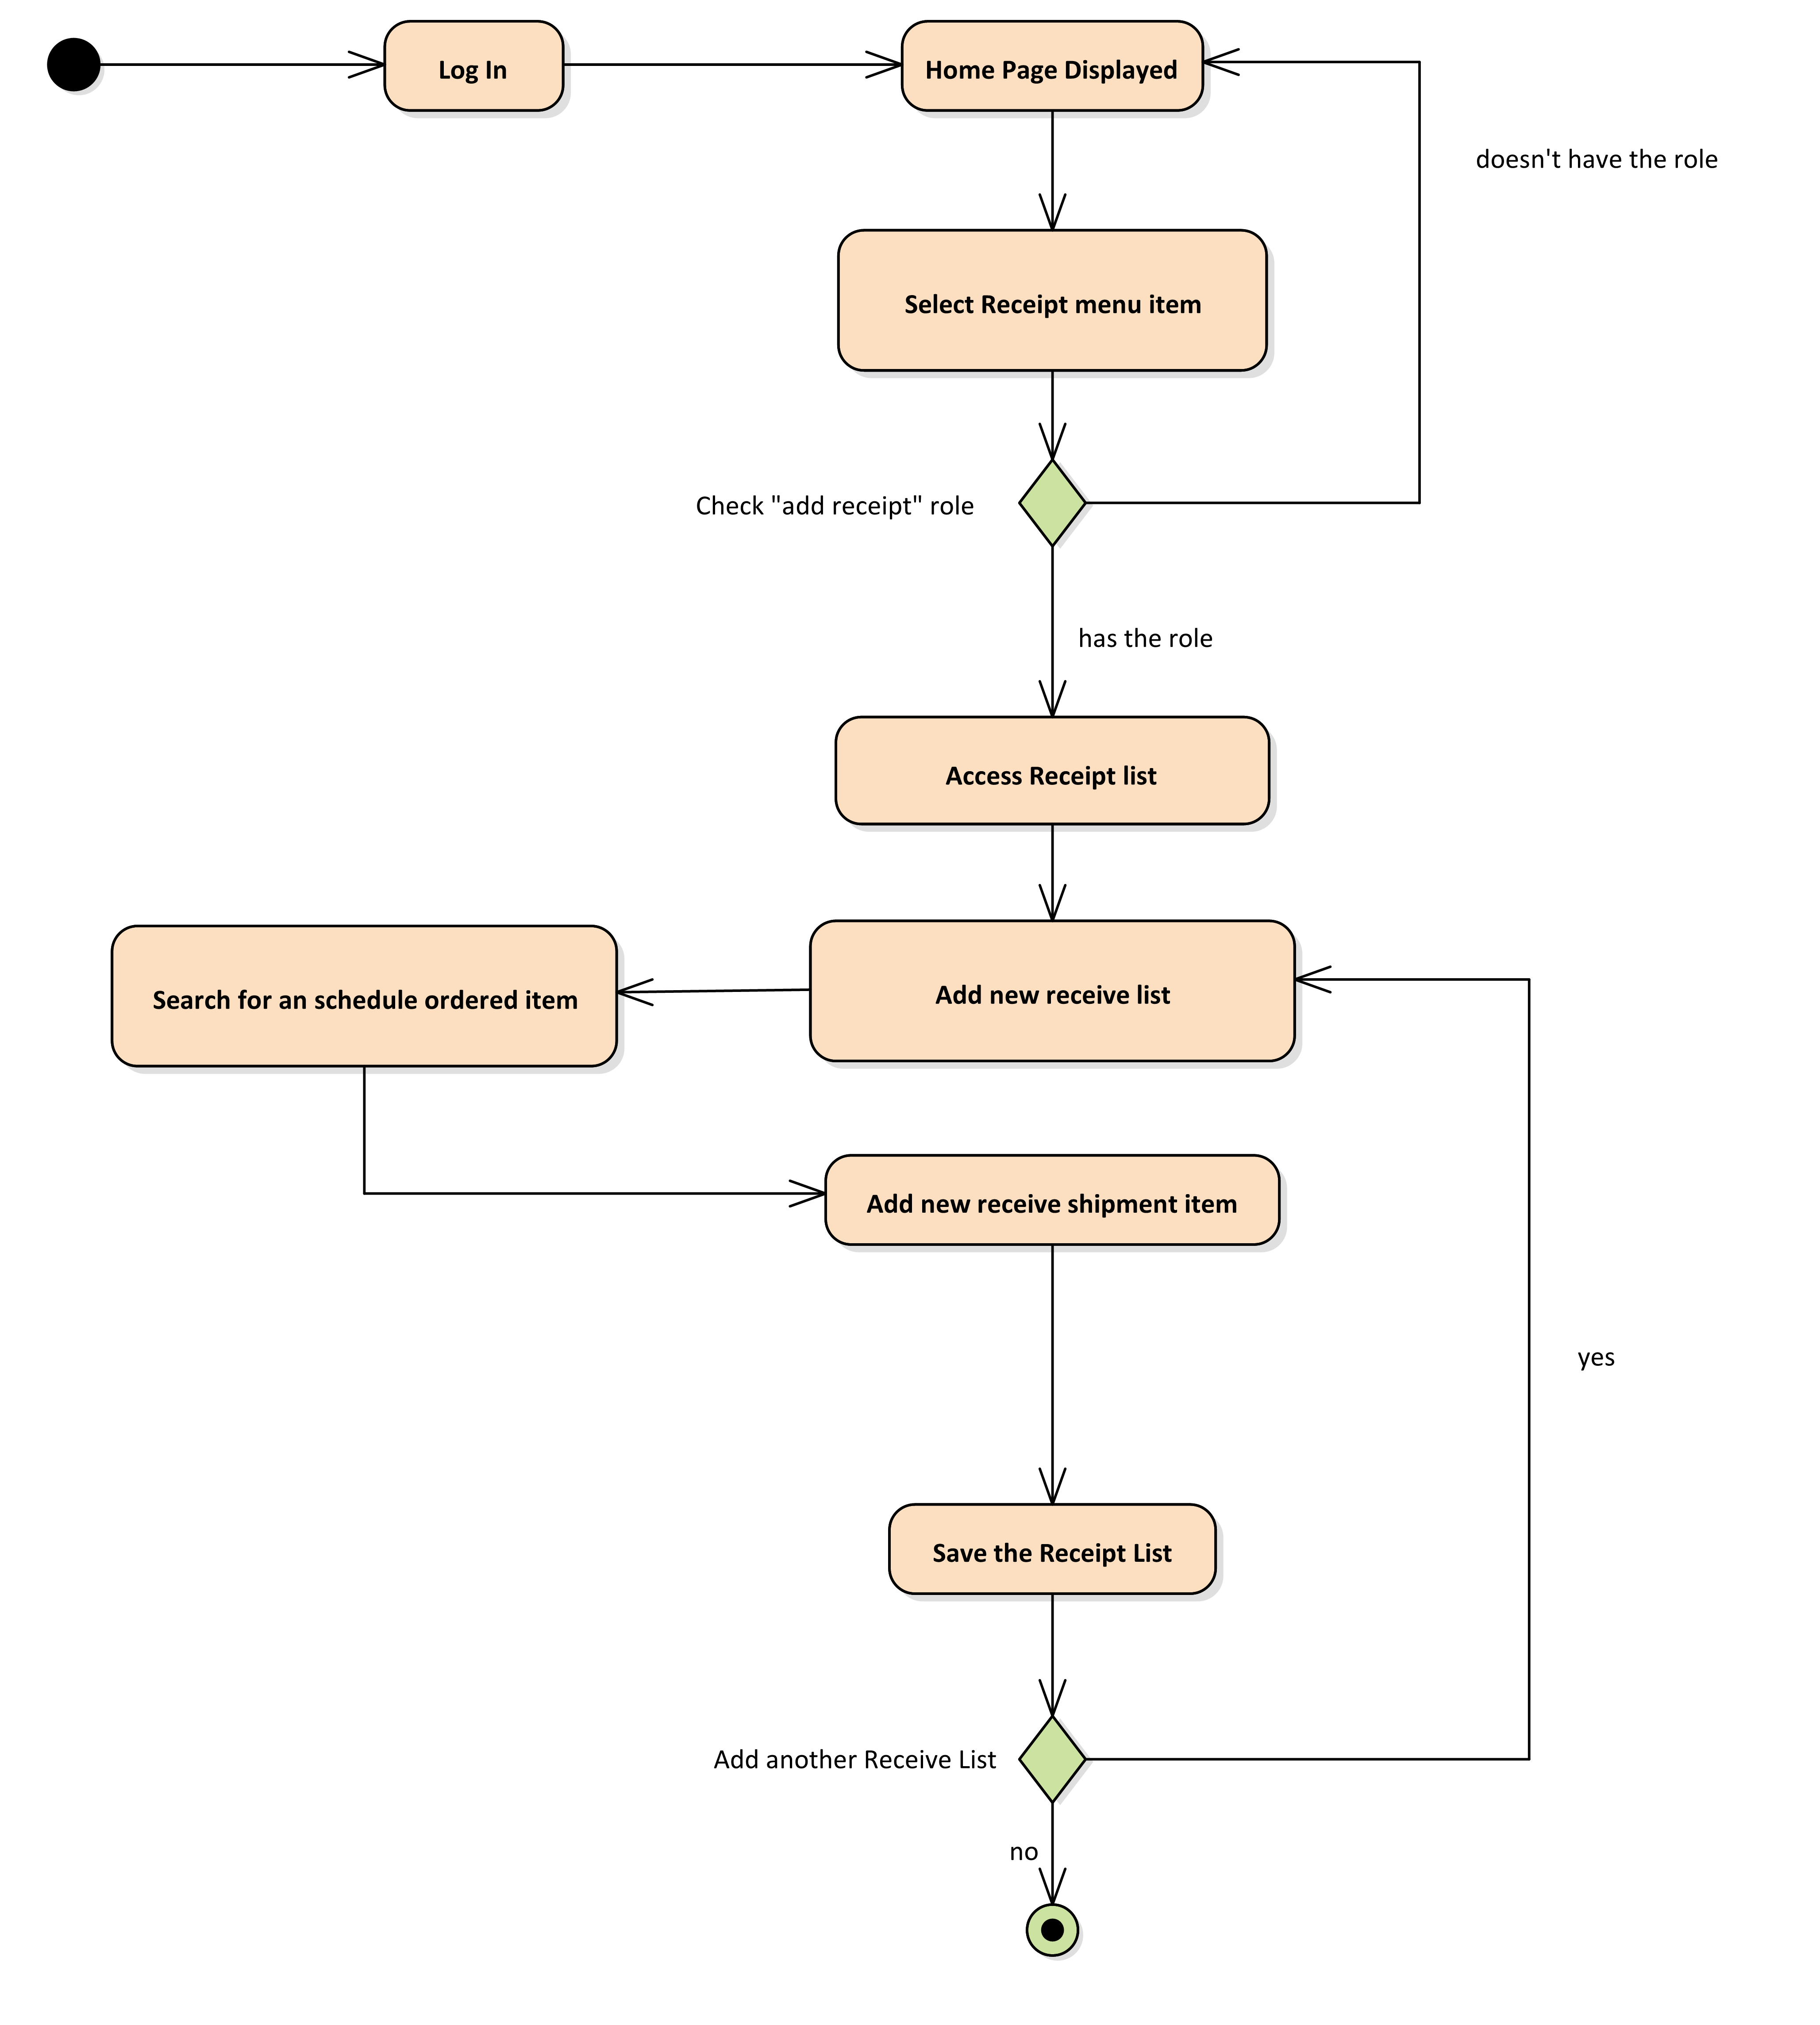
\includegraphics[width=1\textwidth]{pic/Activity/receive.png}
	\caption{Receiving Activity Diagram}
	\label{fig:receive}
\end{figure}
% all Activity commenting================
% all Activity commenting================

\fi
\clearpage


\subsection{Class Diagram}
The Class diagram represents classes, their component parts, and the way in which classes of objects are related to one another. A class diagram is a diagram describing the structure of the system. Used for capturing requirements and end user interaction.\\

\begin{figure}[h]
	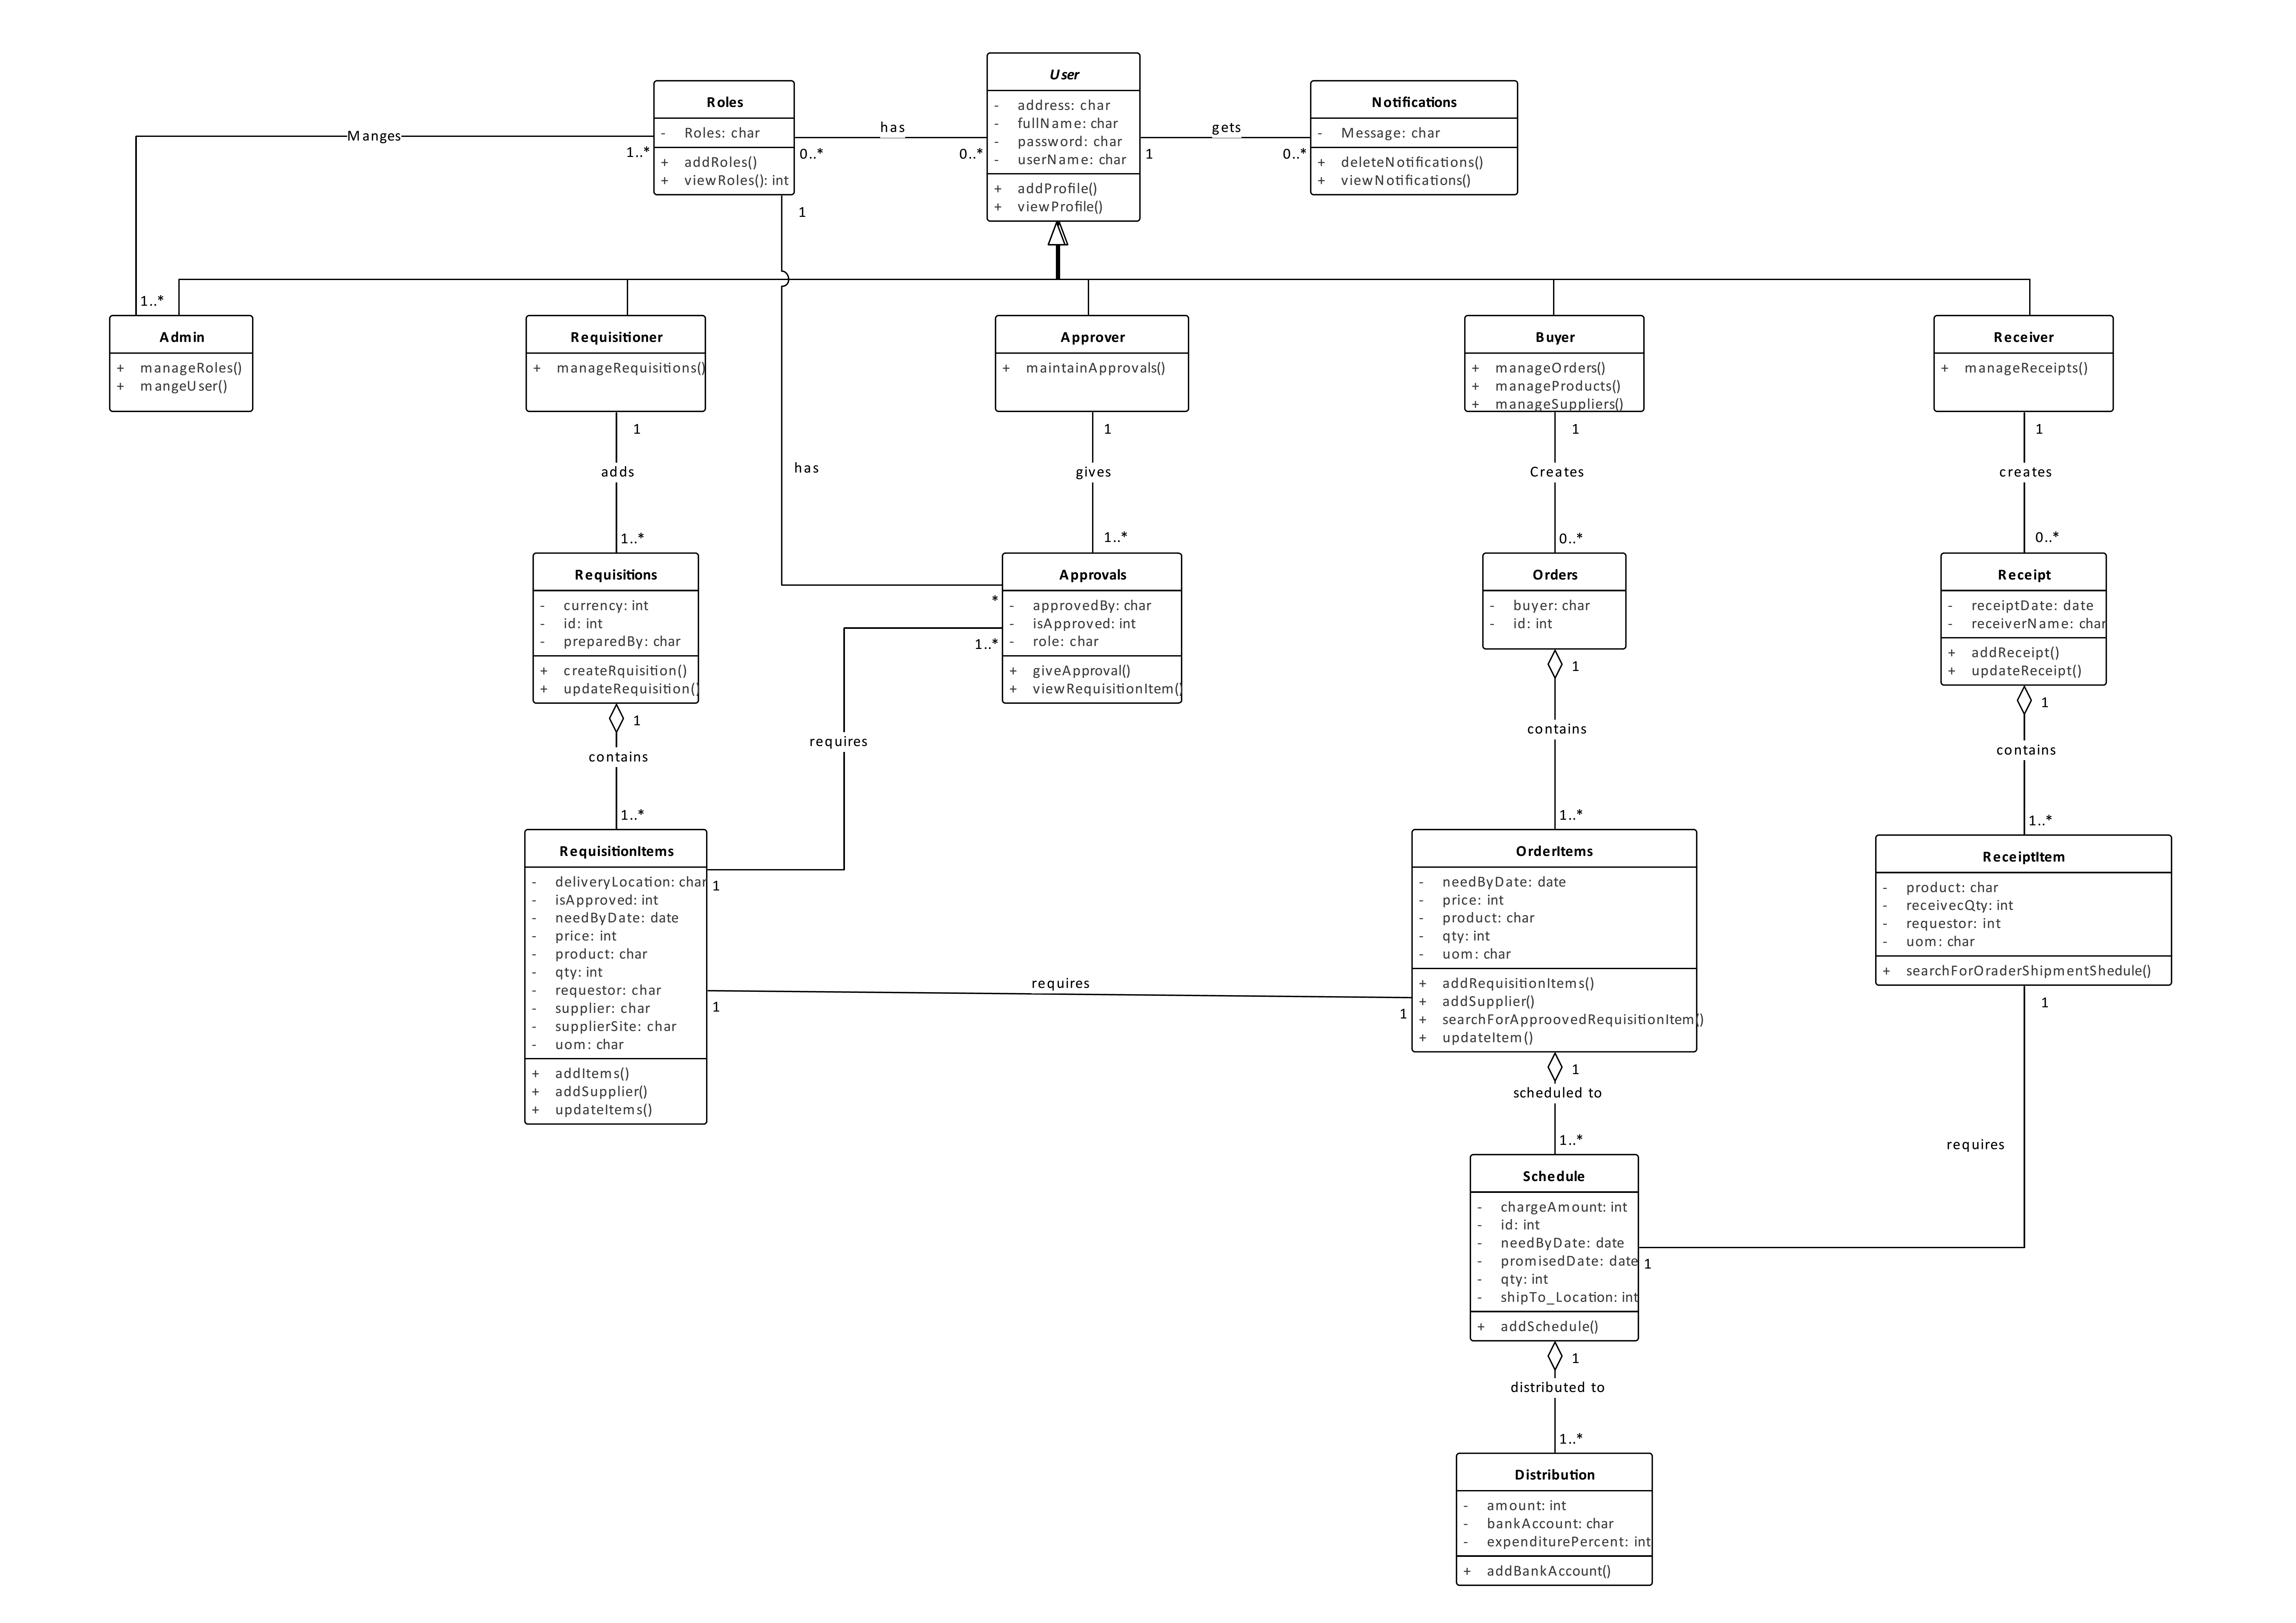
\includegraphics[width=1.1\textwidth]{pic/class/seupr_class.png}
	\caption{SEU Purchase Requisition Class Diagram}
	\label{fig:Class_Diagram}
\end{figure}
\clearpage



\subsection{Entity Relationship Diagram}
ERD describes the conceptual database design for the end users and represents  main components of database: entities, attributes, and relationships. ERD describes how many tables is needed and what would be the relationship between them. ERD is simple and easy for the representation of a database. It helps a lot to understand the whole database.\\

\begin{figure}[h]
	\begin{center}
	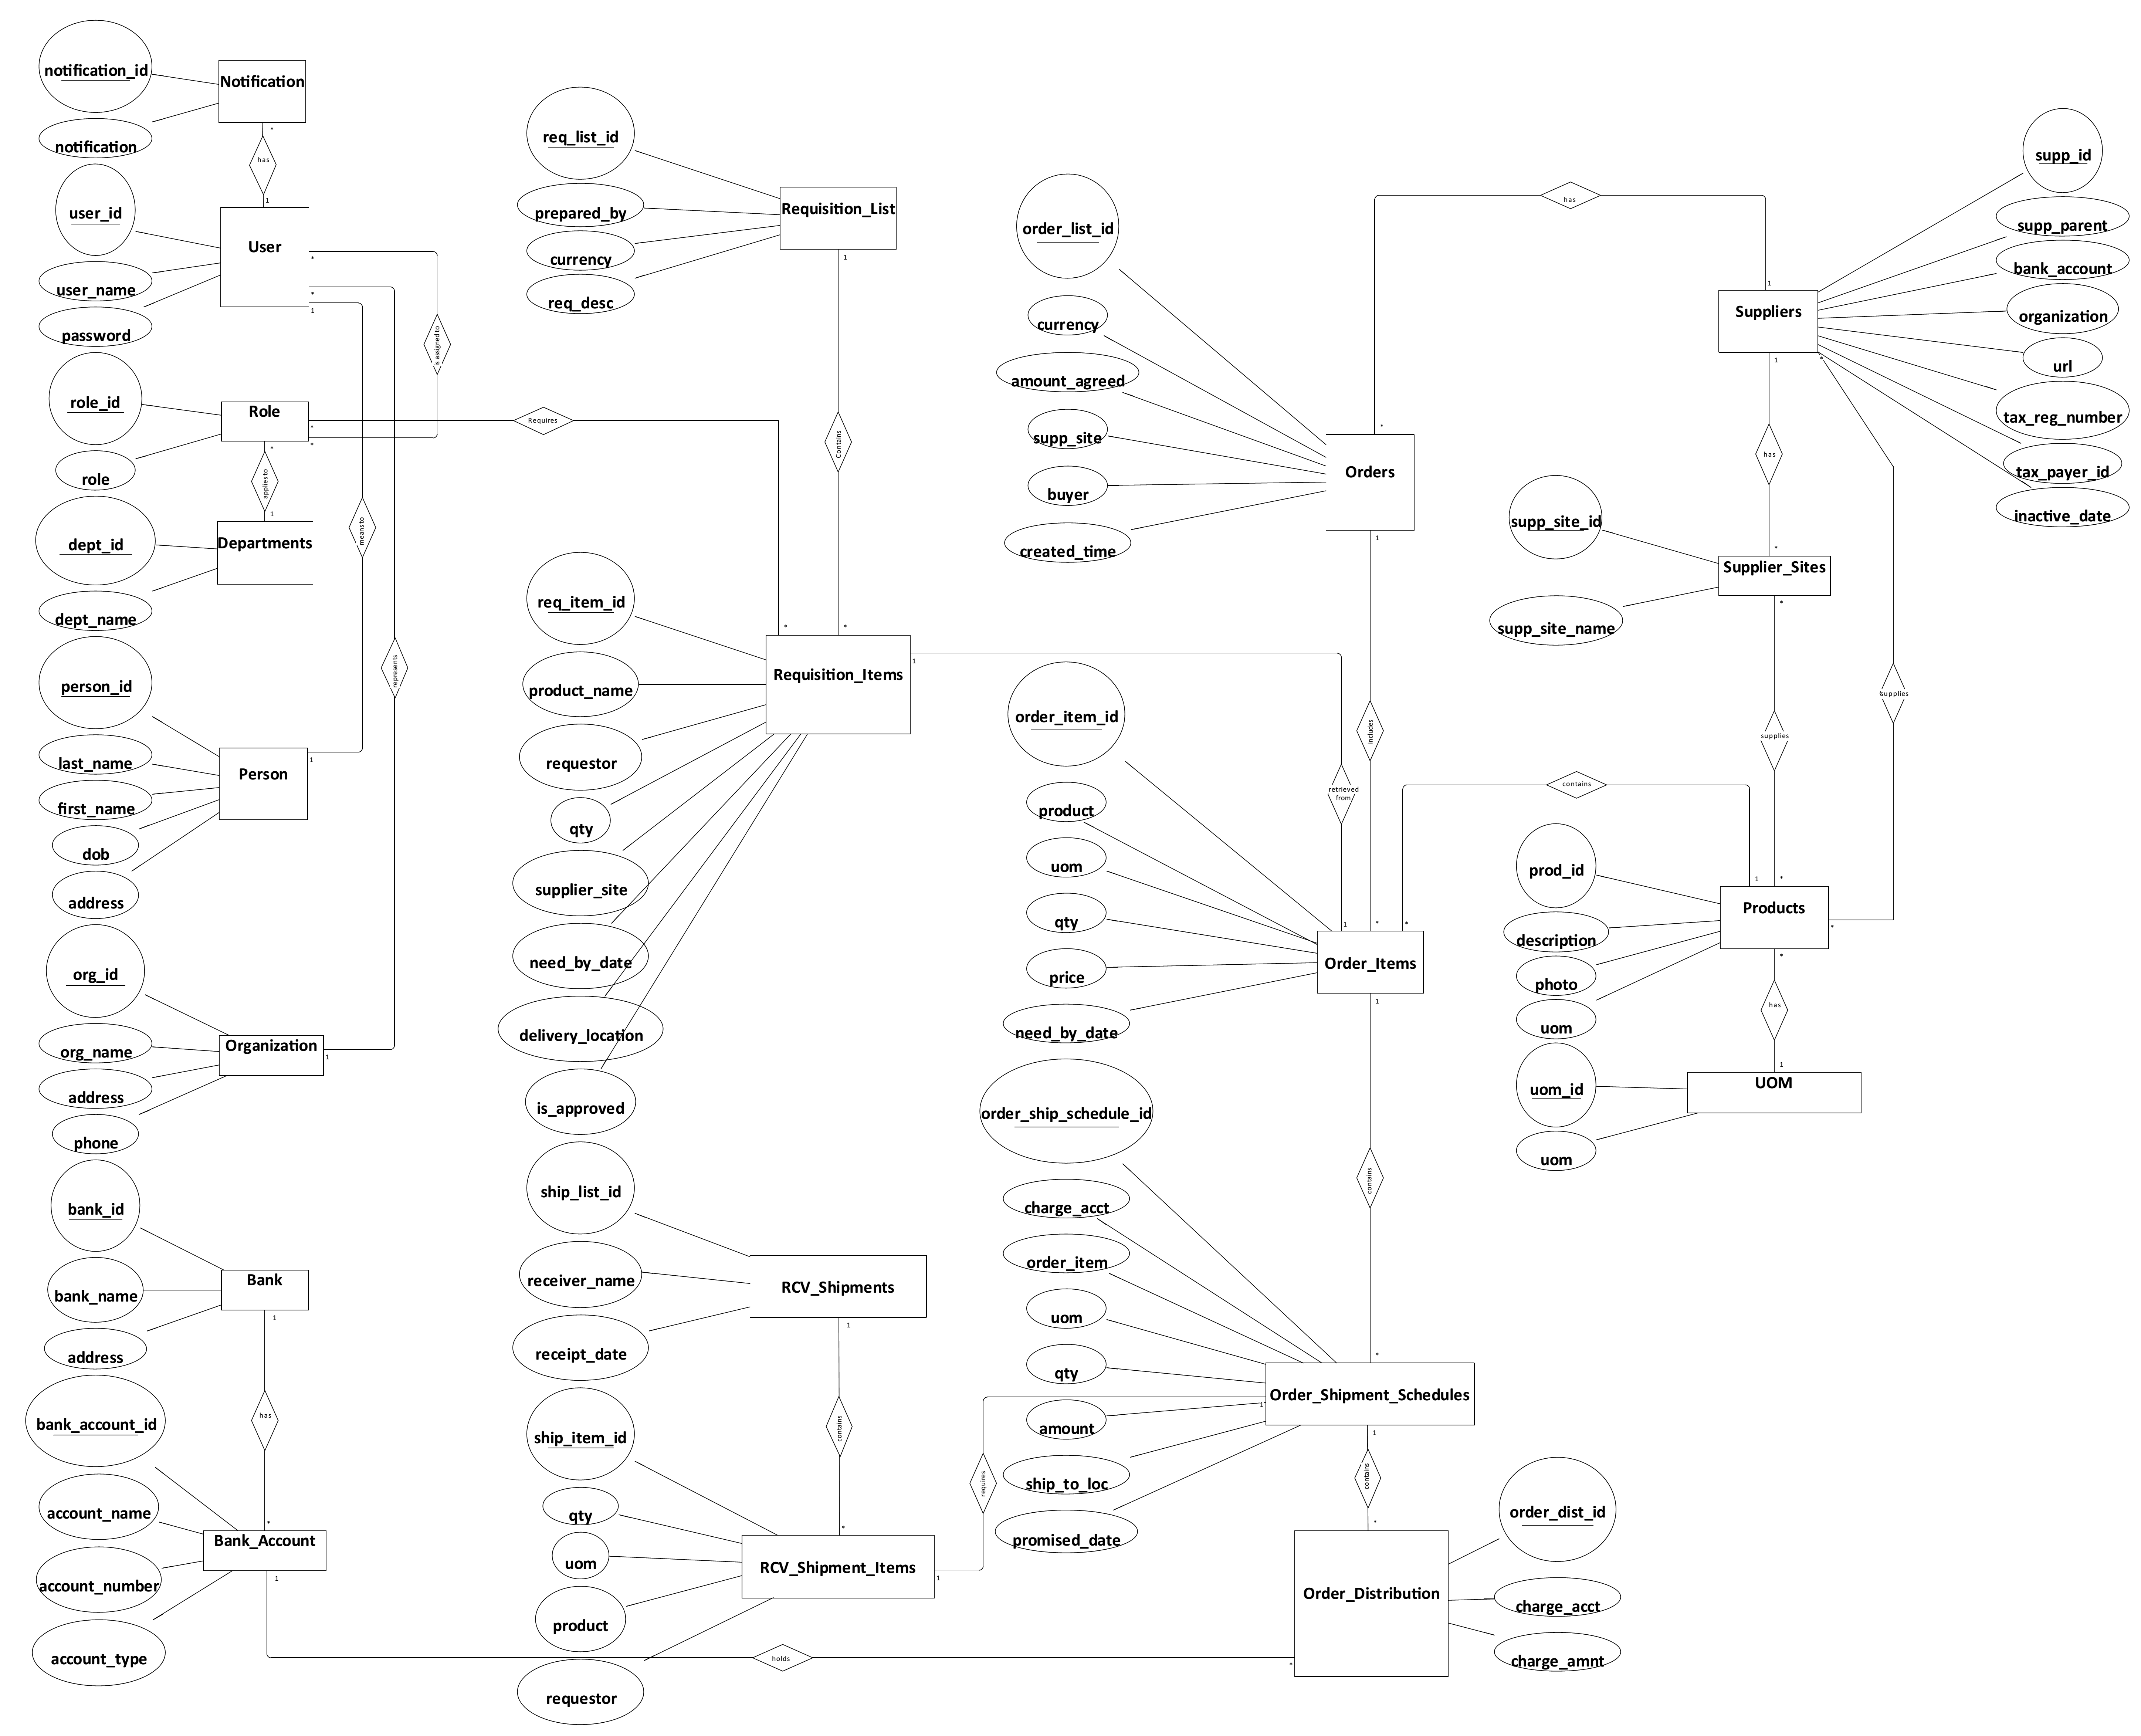
\includegraphics[width=1.1\textwidth]{pic/erd/erd_full.png}
	\end{center}
	\caption{SEU Purcase Requisition Management System ERD}
	\label{fig:erd_full1}
\end{figure}
\clearpage

In, Figure-\ref{fig:erd_full1} the Entity Relationship Diagram of SEU Purchase Requisition Management System project is provided. This diagram is a graphical representation of this project's information system that shows the relationships of entity sets stored in a database. This ER diagrams illustrate the logical structure of physical databases of this project.









%================DFD==============================
%================DFD==============================
\subsection{DFD (Data Flow Diagram)}
Generally DFD shows the Flow of data but not order of events through the system. It is used for general or business purpose only. It is also known as Data Flow Graph and Bubble Chart.

\begin{figure}[h]
	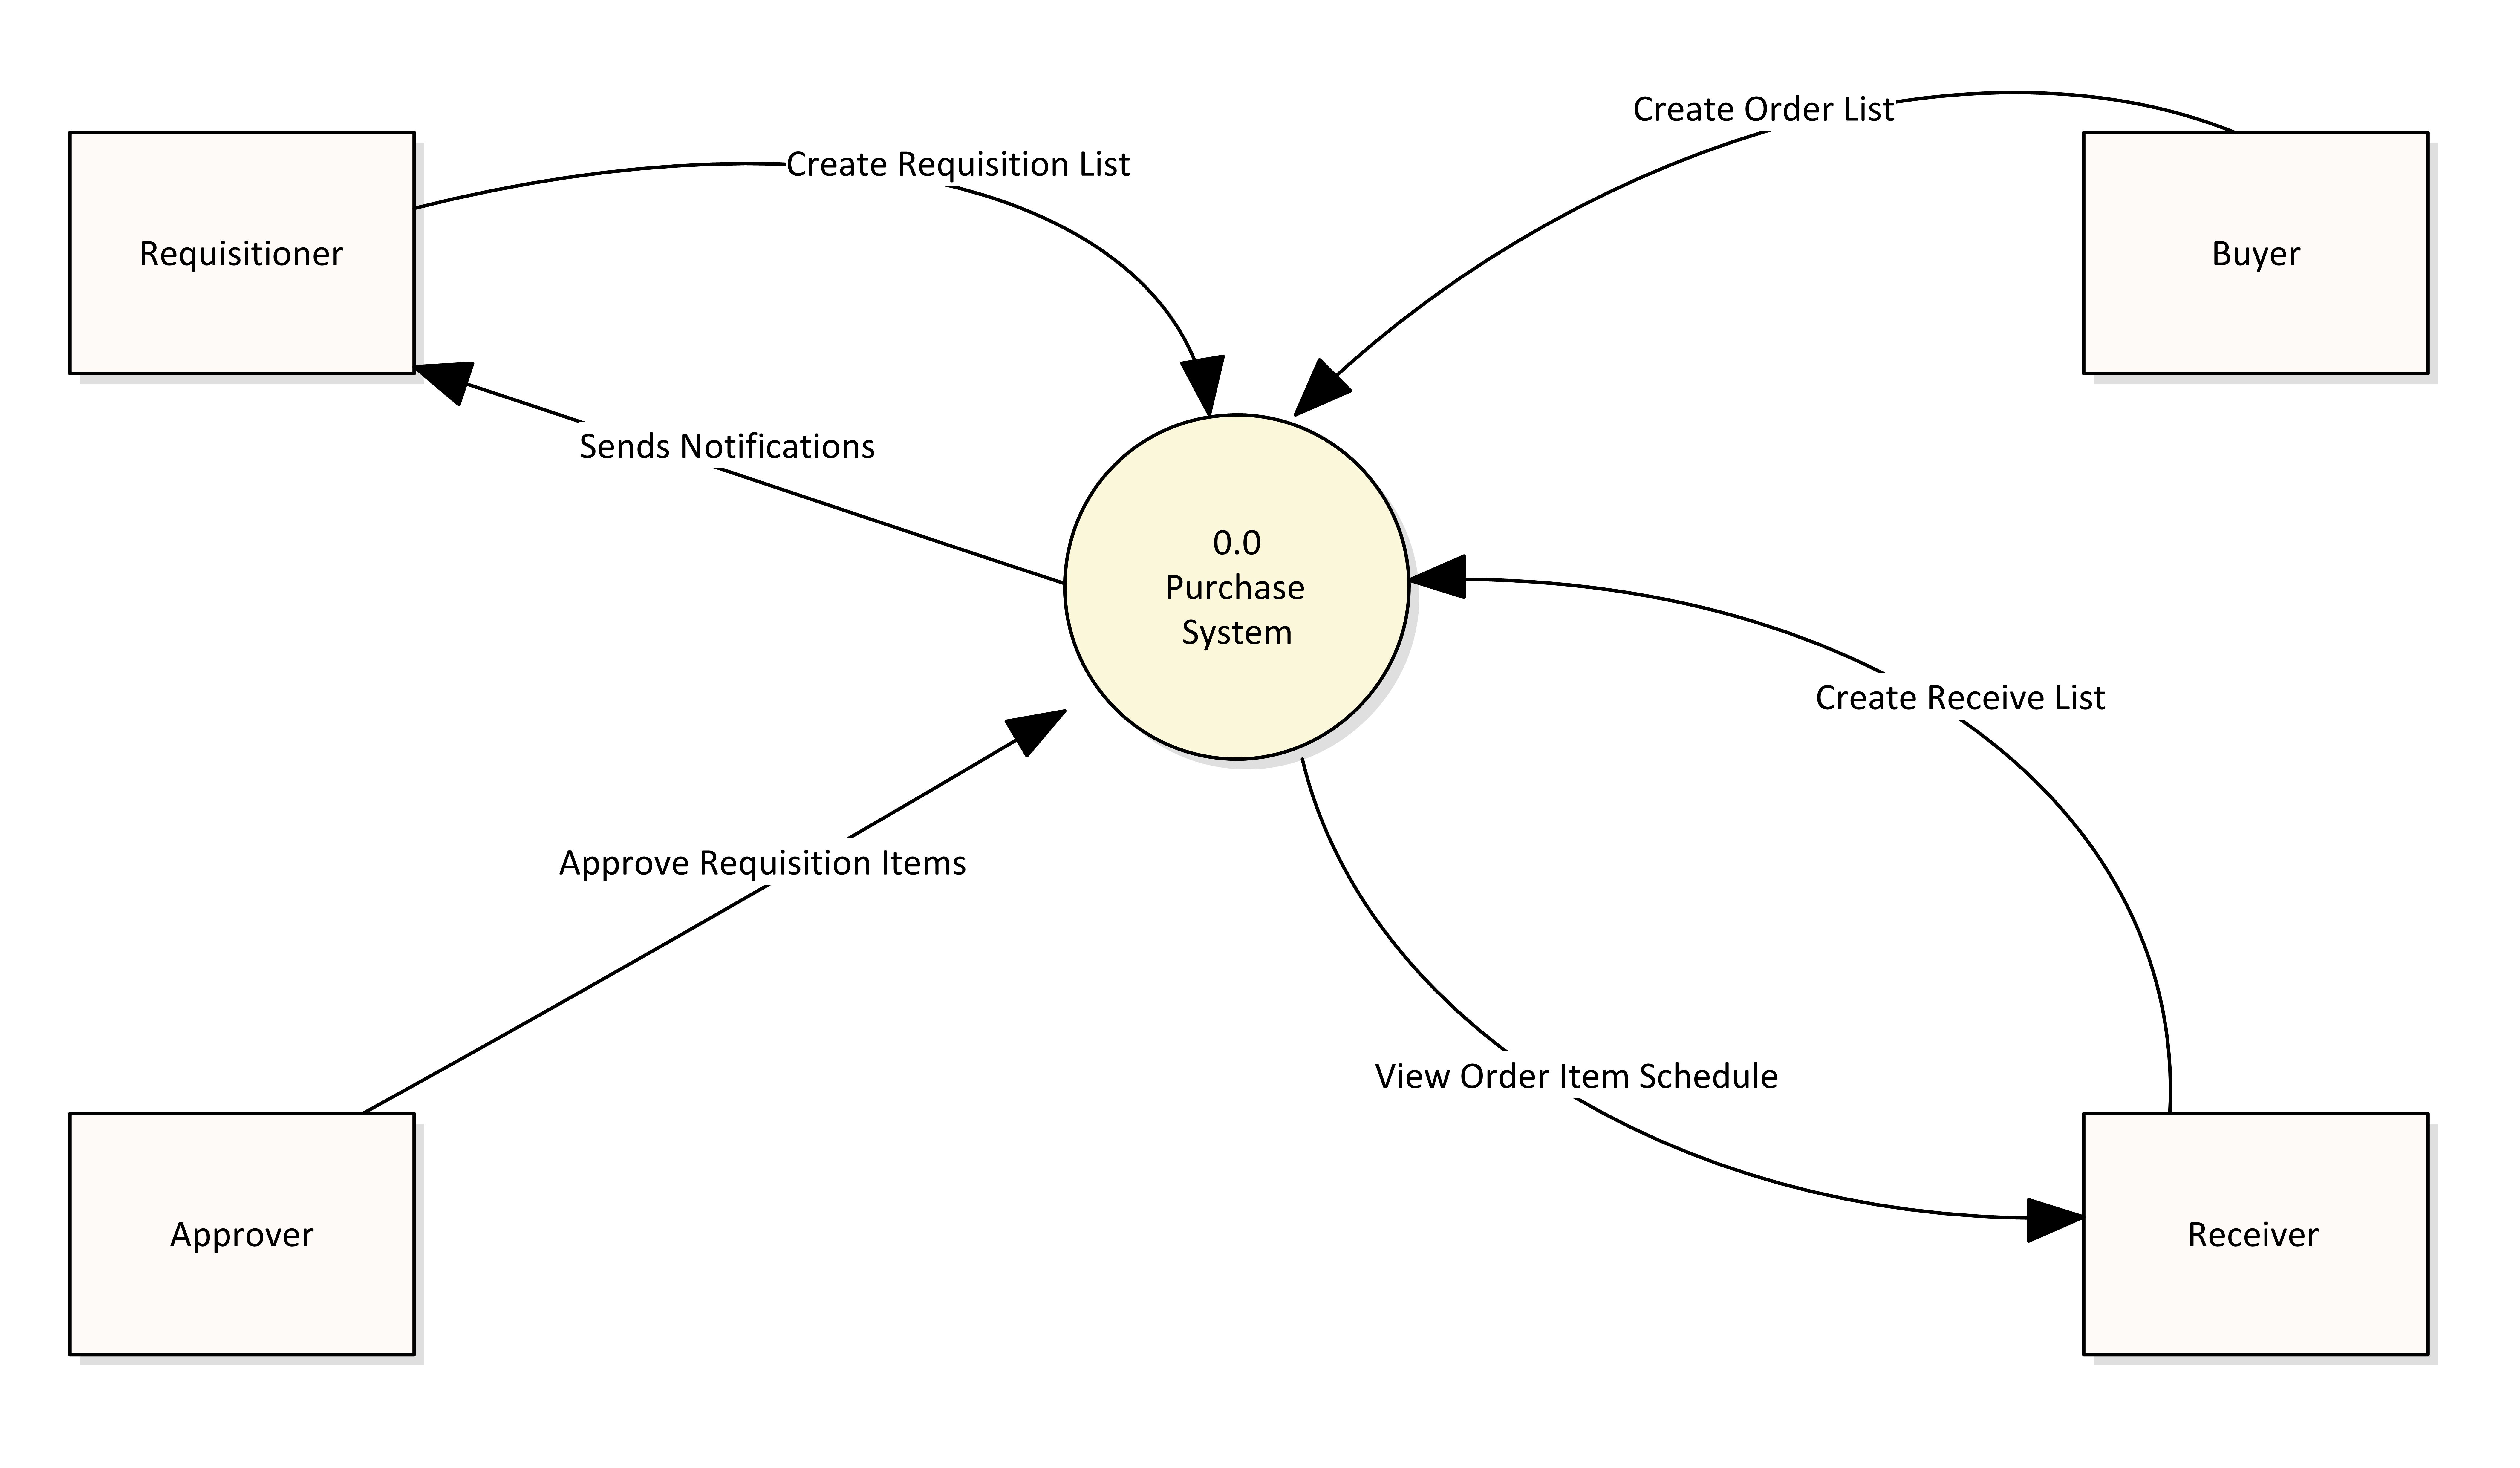
\includegraphics[width=1\textwidth]{pic/DFD/context_level.png}
	\caption{A context level DFD of SEU Purchase Requisition}
	\label{fig:context_level}
\end{figure}
\clearpage


%================Schema Diagram==============================
%================Schema Diagram==============================



\newgeometry{bottom=1cm,left=1cm, top=0cm, right=0cm}
\begin{landscape}
\subsection{Schema Diagram}
\begin{figure}[h]
	\begin{center}
		%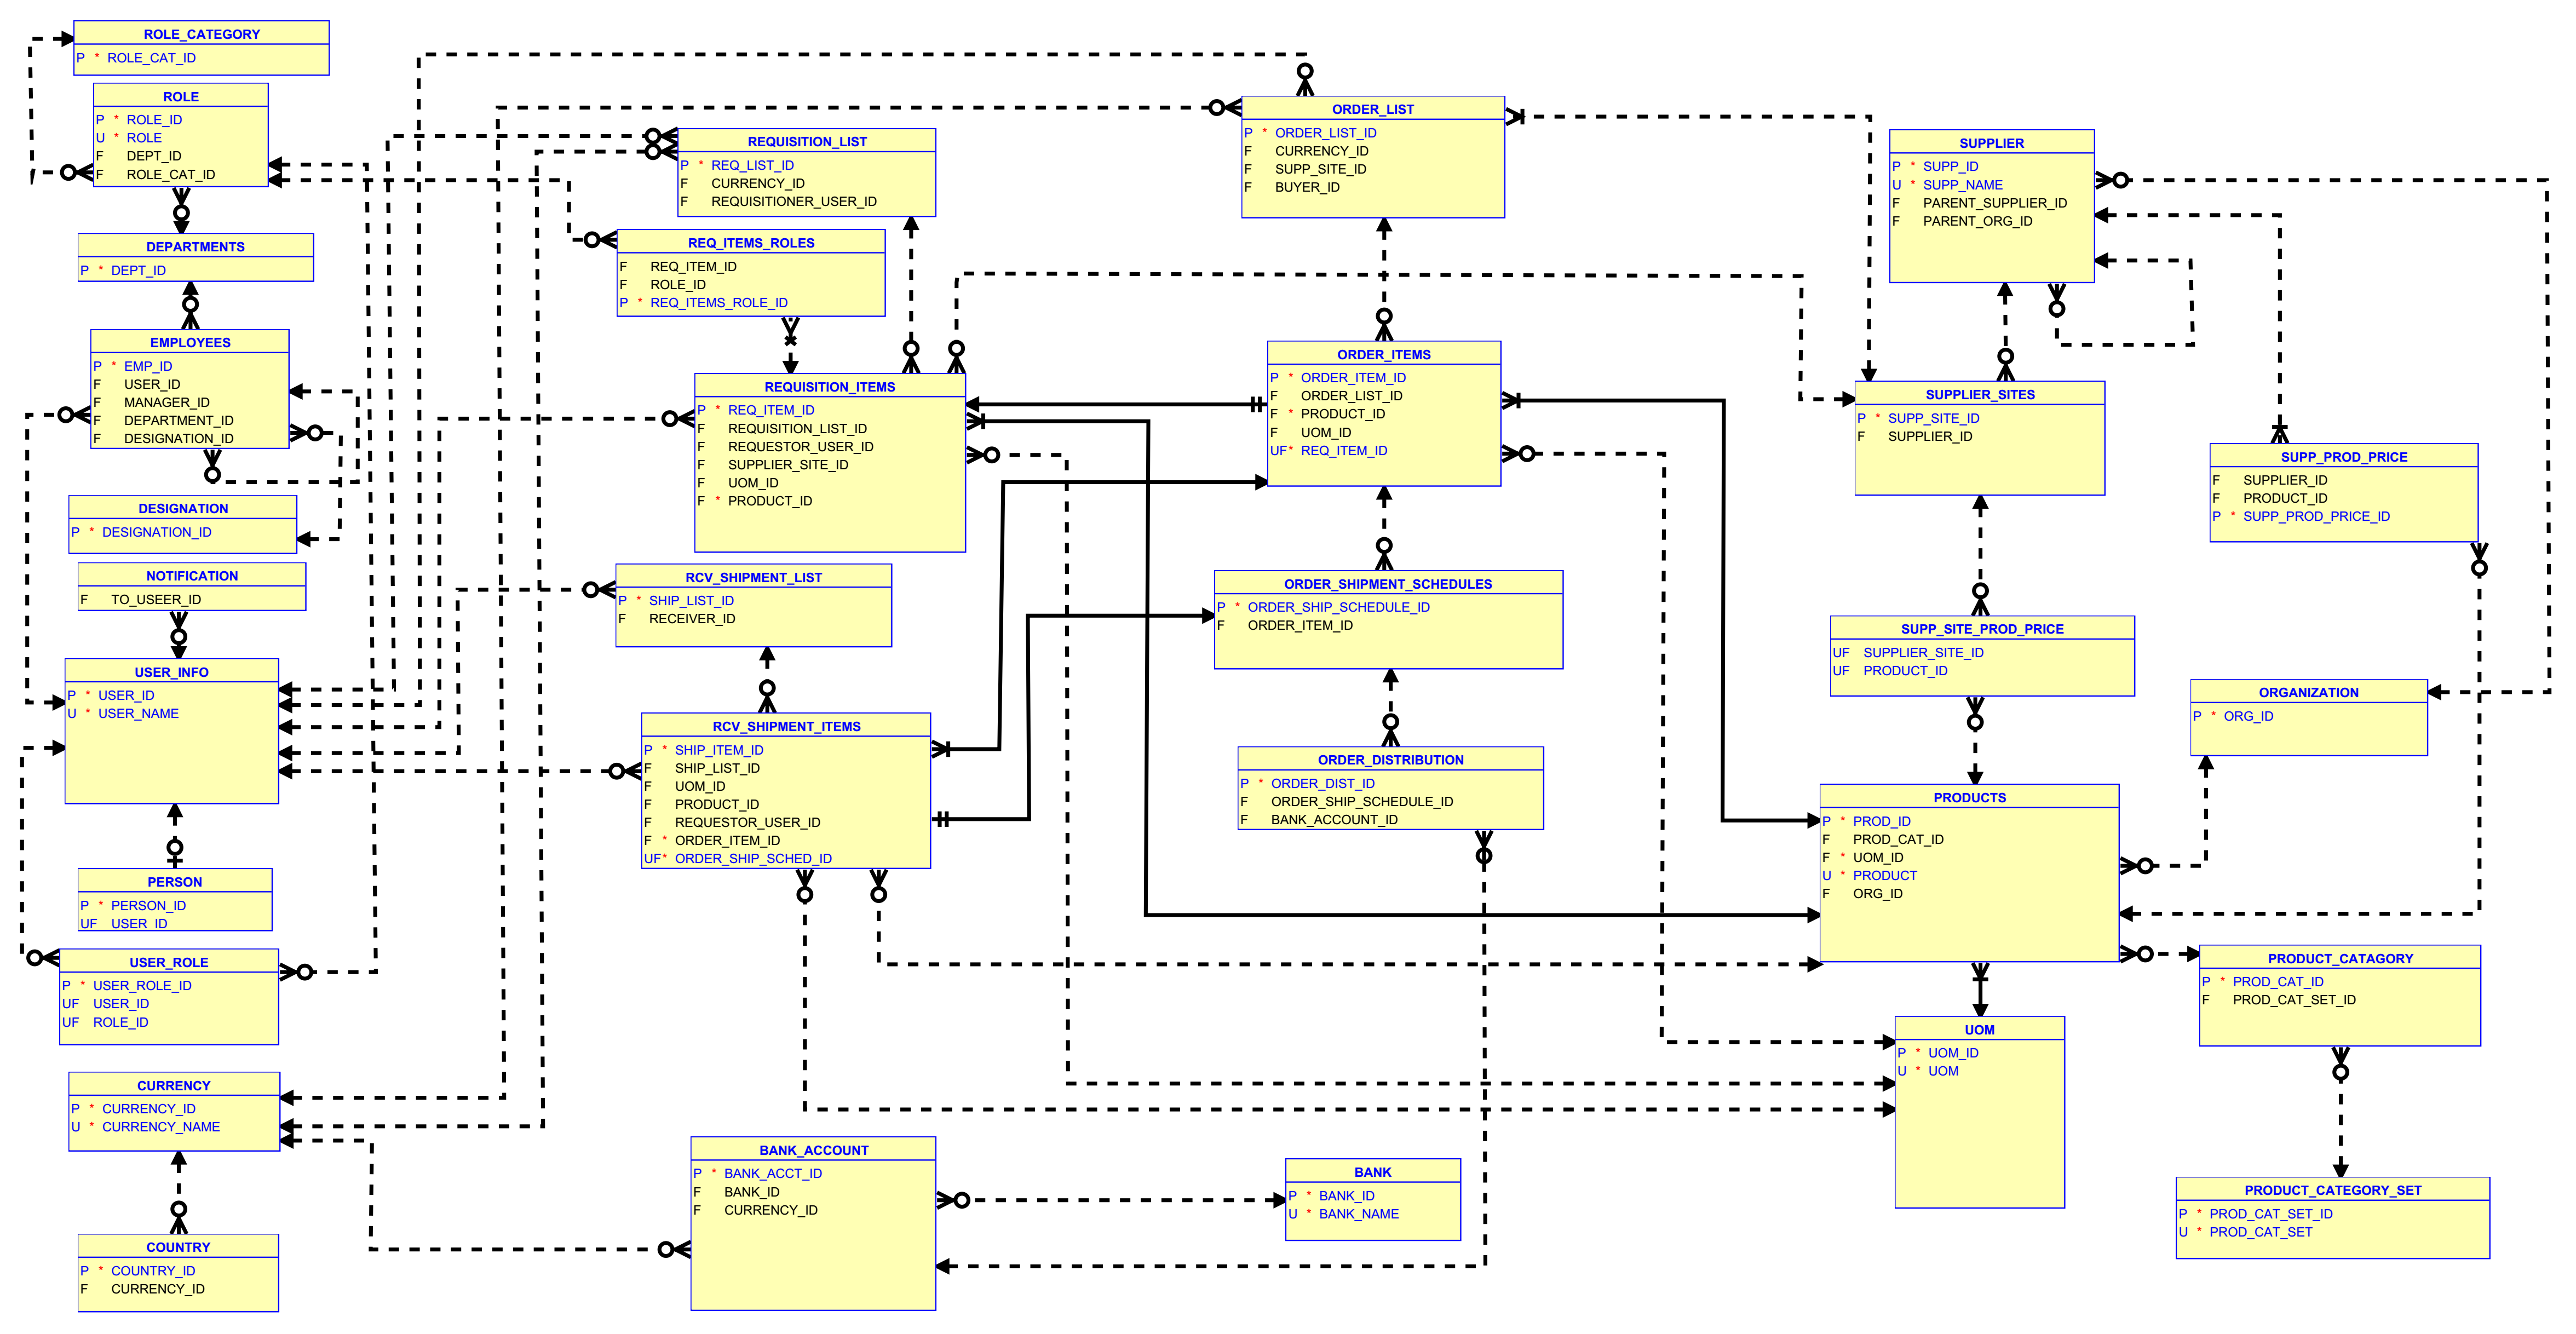
\includegraphics[width=0.95\textwidth, angle =90]{pic/schema/seupr_schema.png}
		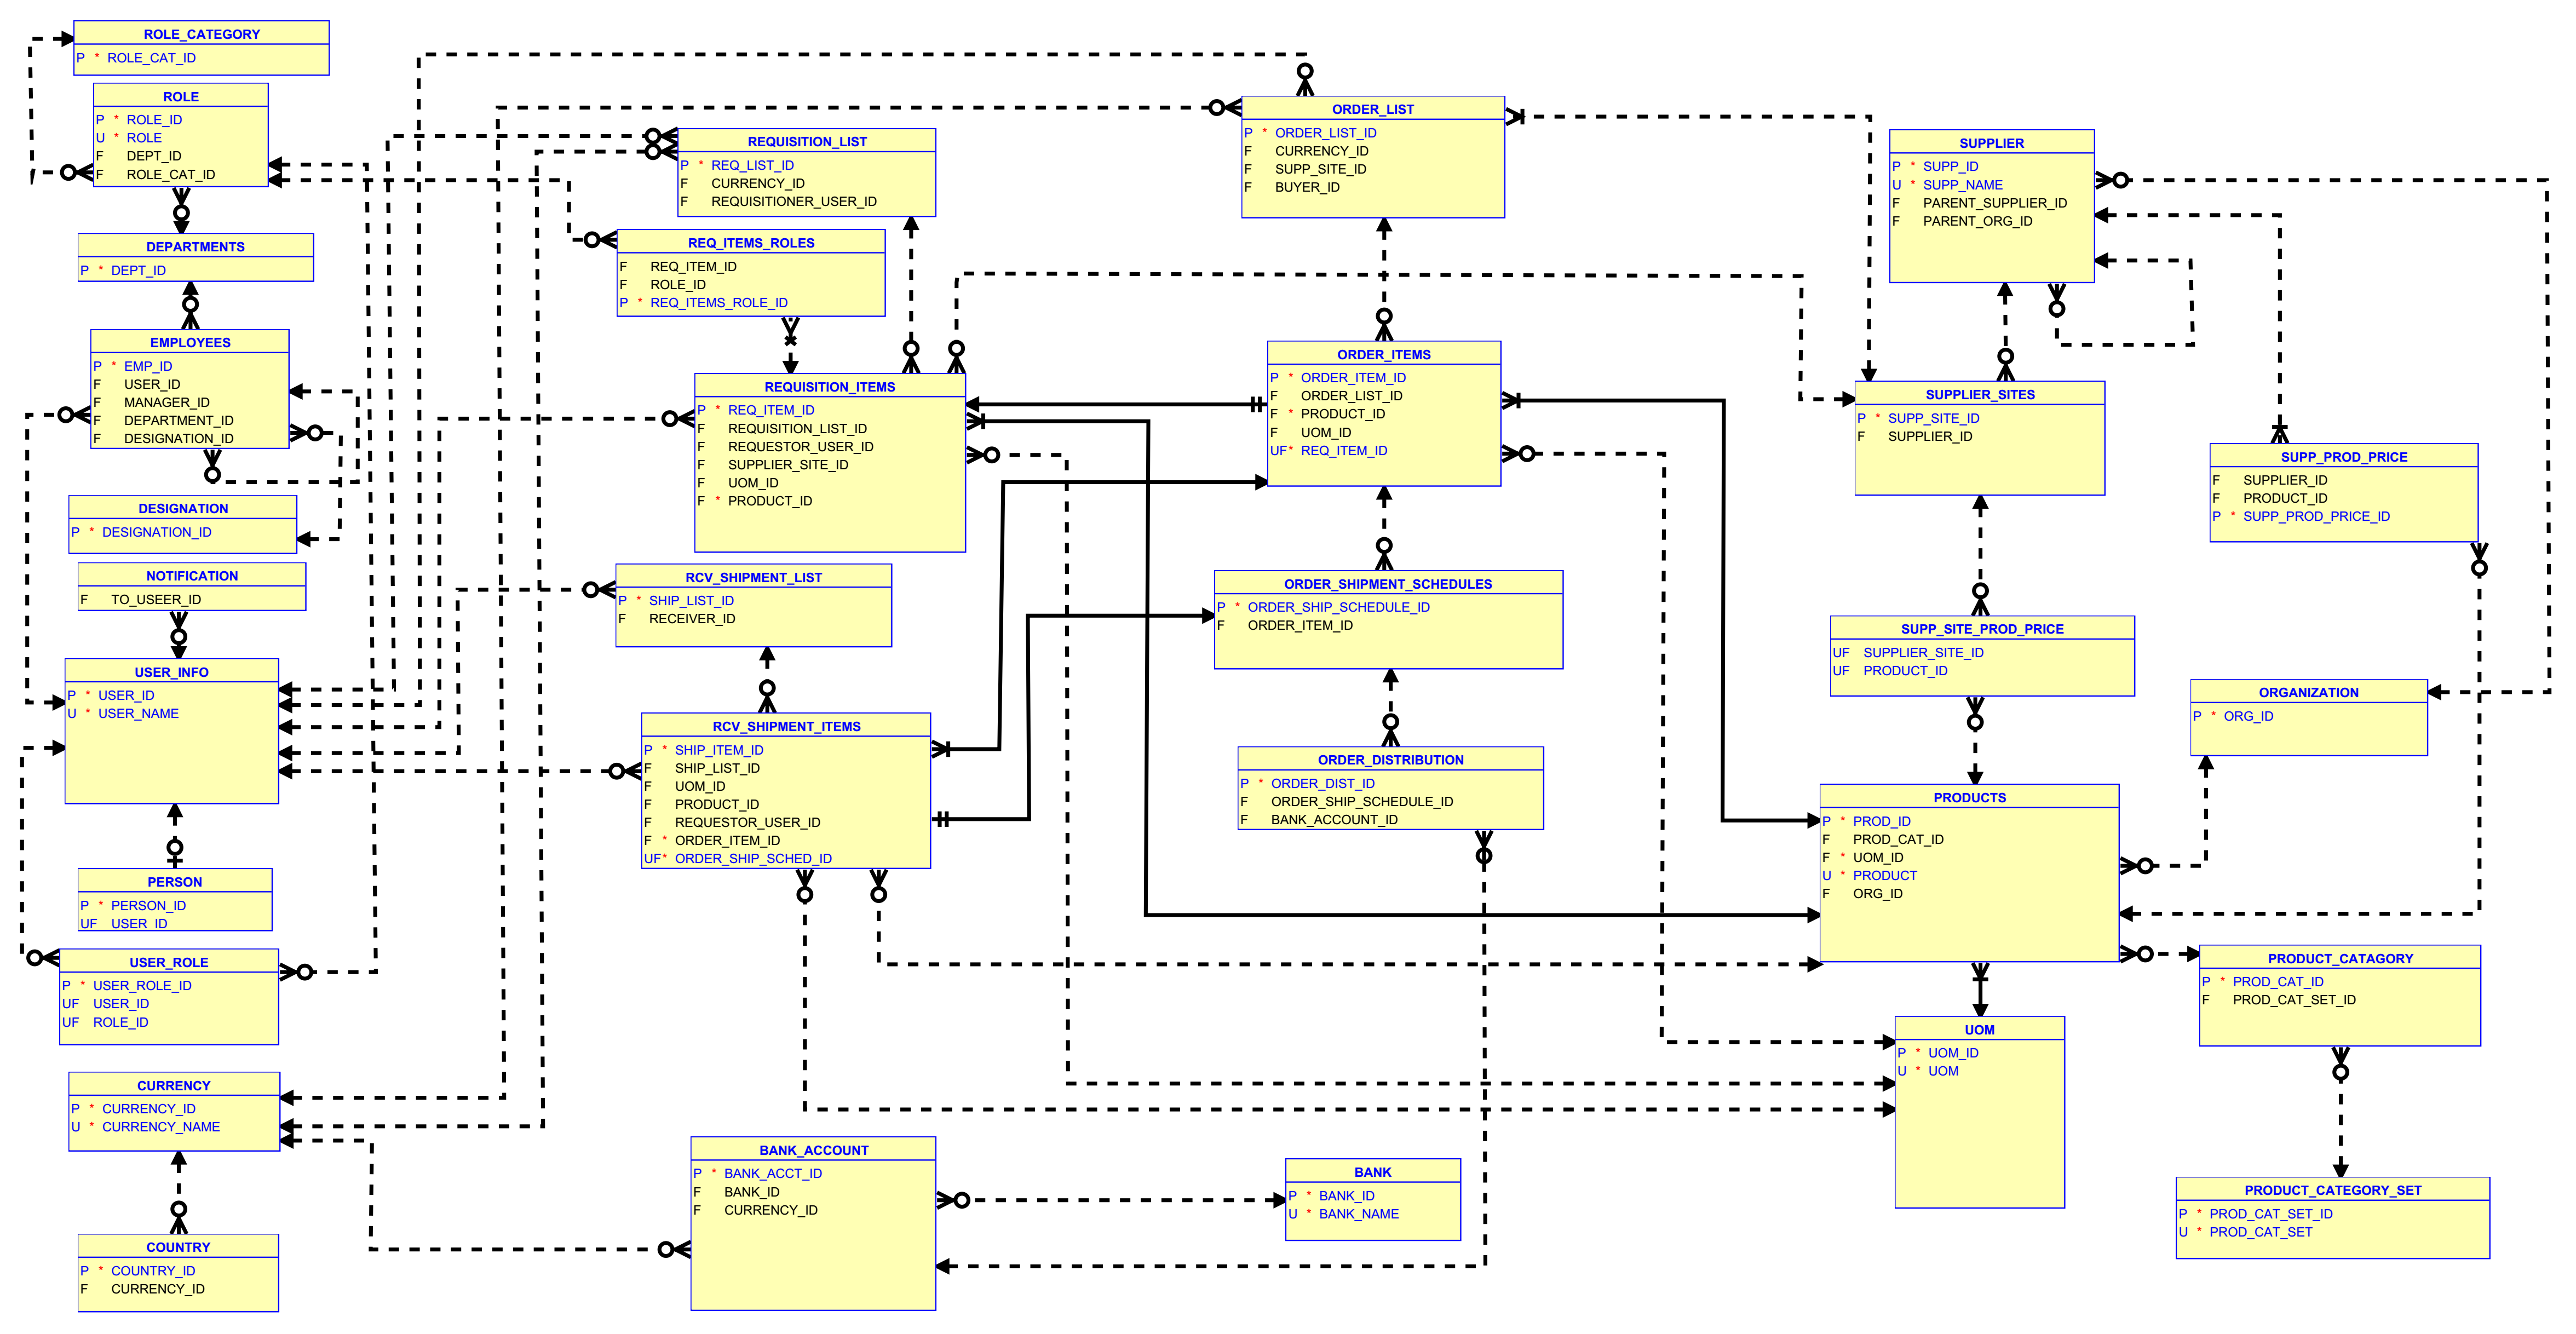
\includegraphics[width=1.3\textwidth]{pic/schema/seupr_schema.png}
	\end{center}
	\caption{Schema Diagram of SEU Purchase Requisition}
	\label{fig:context_level}
\end{figure}
\thispagestyle{empty} 
\end{landscape}

\restoregeometry




\ifx
\newgeometry{bottom=1cm,left=1cm, top=0cm, right=0cm}
\begin{landscape}
\subsection{Activity Diagram}
\begin{figure}[h]
%Activity diagrams combination of activities for a system and represents the flow of use cases and work-flows of step-wise activities and actions. The activity is described as operation in the system. Activity diagram can show that are conditional or parallel. \\

	\begin{center}
	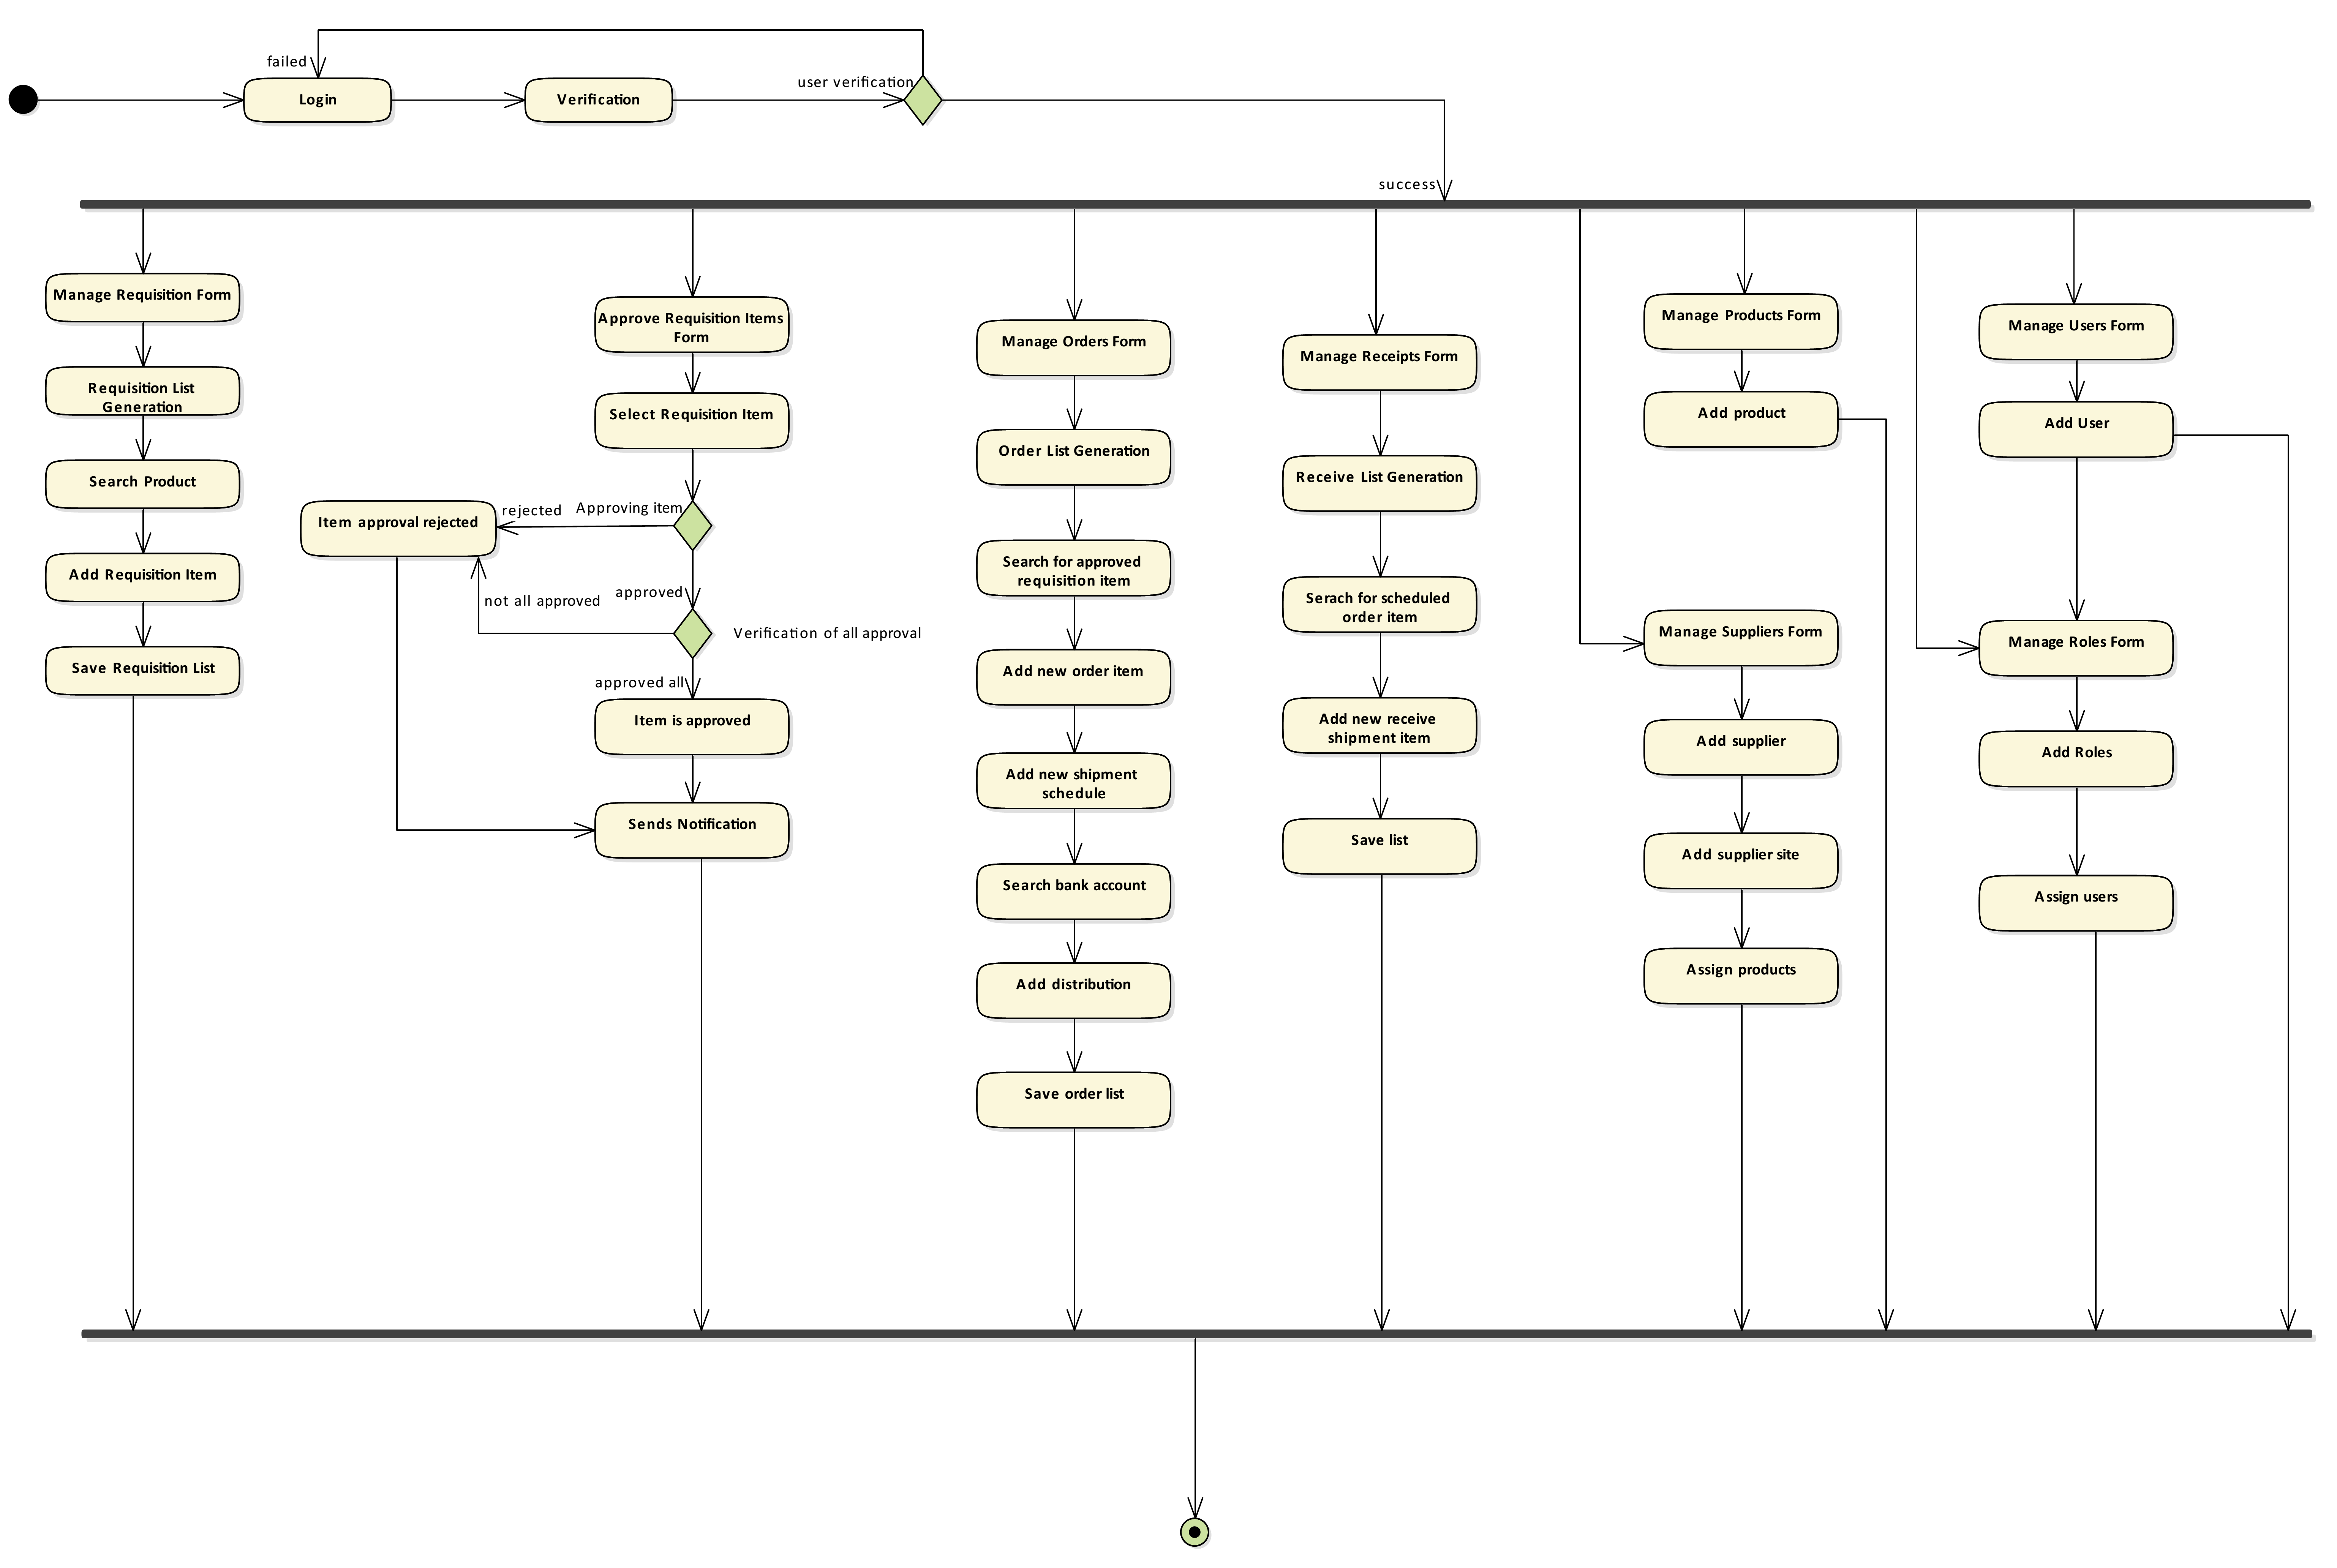
\includegraphics[width=1.06\textwidth]{pic/Activity/seupr_full_activity.png}
	\end{center}
	\caption{SEU Purchase Requisition Activity Diagram}
	\label{fig:activity}
\end{figure}
%\clearpage
\thispagestyle{empty} 
\end{landscape}
%\clearpage

\restoregeometry
\fi




%================Deployment Diagram==============================
%================Deployment Diagram==============================
\subsection{Deployment Diagram : Modeling a client/server system}

\begin{figure}[h]
	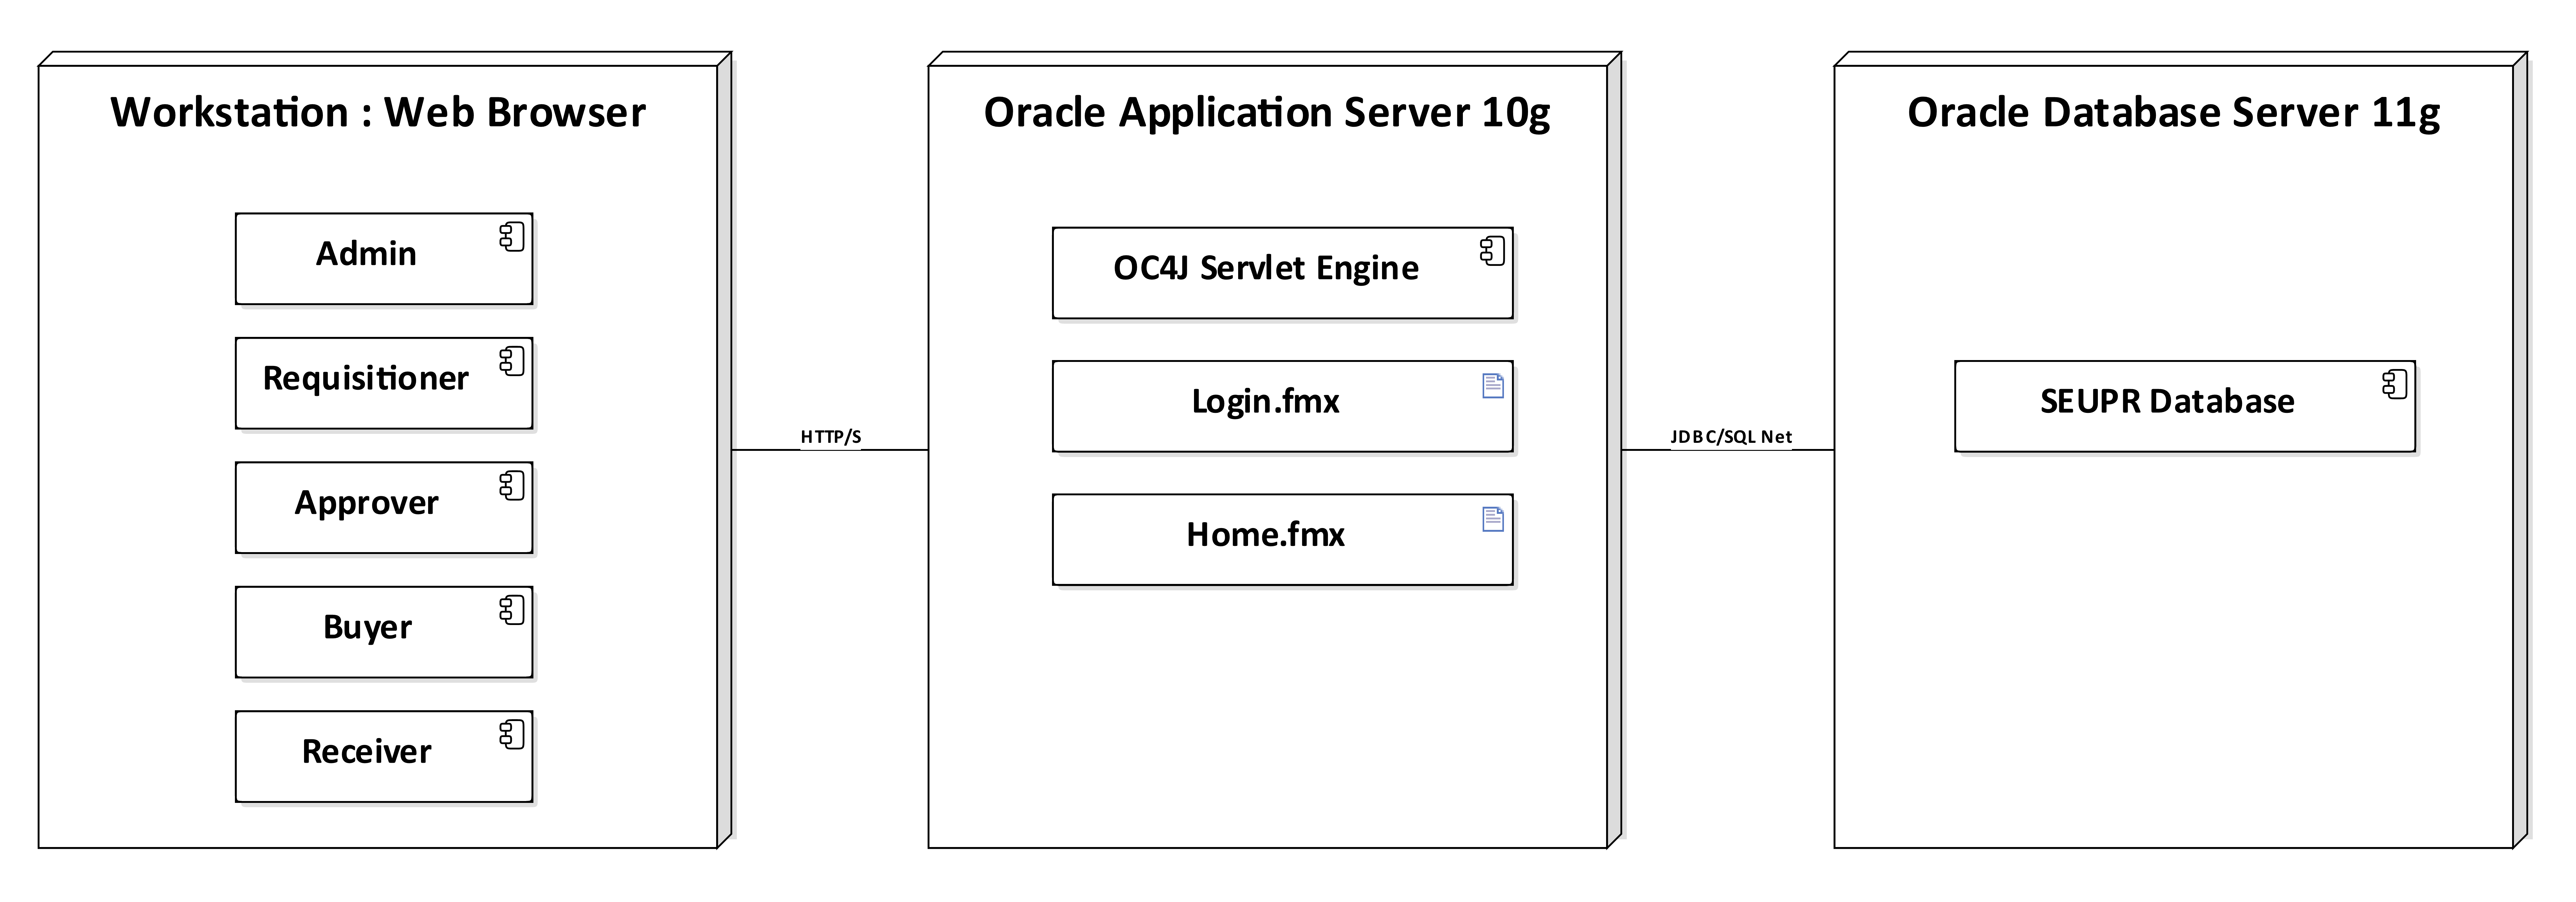
\includegraphics[width=1.1\textwidth]{pic/deployment/client_server.png}
	\caption{A client/server system deployment diagram of SEU Purchase Requisition}
	\label{fig:client_server}
\end{figure}


\paragraph{Oracle Forms Services :}
Oracle Forms Services uses a three-tier architecture to deploy database applications:\cite{form_builder_book}  \label{sec:form_builder_book_1}
\begin{enumerate}
	\item	The client tier contains the Web browser, where the application is displayed and used.
	\item	The middle tier is the application server, where the application logic and server software reside.
	\item	The database tier is the database server, where enterprise data is stored.
\end{enumerate}

\paragraph{Running a Form : Browser}
\renewcommand{\labelenumi}{\alph{enumi})}
\begin{enumerate}
	\item http://seupr.com:8889/forms/frmservlet?config=seupr
\end{enumerate}
\clearpage
SEU purchase requisition's URL consists of those components\\

\begin{table}
\begin{tabular}{|l|l|}
\hline
 Protocol & http \\
\hline
 Host and domain & seupr.com\\
 \hline
 Port for HTTP Server or OC4J  & 
 \vtop{
 		\hbox{\strut 80 default for HTTP Server}				
 		\hbox{\strut 8889 default for OC4J}
	}\\
\hline
 Forms Servlet Alias or static HTML file & /forms/frmservlet \\
 \hline
 Parameters: This section begins with “?" & config=seupr\\
\hline

\end{tabular}
\end{table}

\clearpage





%\section{Testing}




\chapter{Tools}
%\section{Goals}
\setcounter{page}{1}

\section{Hardware Requirement} %IS Chapter 5
\renewcommand{\labelenumi}{\alph{enumi})}
	\begin{enumerate}
  		\item A PC with Windows (preferred) operating system.
  		\item RAM is greater than or equivalent to 4 GB
  		\item Intel® Core™2 Duo Processor E8400 or higher  
  		\item Secondary Memory atleast 10 GB
	\end{enumerate}





%\section{Required Tools} 
\section{Software Requirement}
\thispagestyle{empty}    %ADD IMMEDIATELY BEFORE EVERY CHAPTER
\subsection{Front End}
\renewcommand{\labelenumi}{\alph{enumi})}
\begin{enumerate}
  \item Oracle Developer Suite 10g (10.1.2.0.2) 
  	\begin{enumerate}
  		\item Oracle Form Builder [32-bit]
  		\item Oracle Reports Developer
	\end{enumerate}
	
  \item Oracle SQL Developer (4.0.1.14)
  \item SQL*Plus: Release 10.1.0.4.2 - Production
  \item Enterprise Architect 13 
  \item Maxthon Browser [Version: 5.1.6.1000]
  \item Mozilla Firefox Browser [Version: 40.0.1, 32-bit]
  \item Sublime Text 3
\end{enumerate}




\subsection{Back End}
\renewcommand{\labelenumi}{\alph{enumi})}
\begin{enumerate}
  \item Oracle Database 11g Enterprise Edition Release 11.2.0.1.0 - Production
  \item Java SE Development Kit 6u45
\end{enumerate}


\subsection{Supported Platforms}
\renewcommand{\labelenumi}{\alph{enumi})}
\begin{enumerate}
		\item Microsoft Windows (XP, Vista, 7, 8, 10)
		\item macOS
		\item Red Hat Linux
		\item and others
\end{enumerate}

%\section{Features of this Software}
%
%\begin{itemize}
%		\item Role wise user access
%		\item Requisition generation
%		\item Requisition approvals and notifications
%		\item Purchase order generation 
%		\item Supplier, Supplier Sites and Supplier Sites's product price information management
%\end{itemize}

\subsection*{Oracle Forms} 
\renewcommand{\labelenumi}{\alph{enumi})}
\begin{enumerate}
		\item \textbf{What is Oracle Forms?}
		\begin{enumerate}
			\item a component of Oracle Fusion Middleware.
			\item a software product to create GUI for end users
			\item It has an IDE including an object navigator, property sheet and code editor that uses PL/SQL.
			\item originally developed to run server-side .

		\end{enumerate}
		
		\item \textbf{Why Oracle Forms is being used?}
		\begin{enumerate}
			\item It is Oracle's long-established technology to design and build enterprise applications quickly and efficiently.
			\item Development the way you want it .
			\item Simple and fast.
			\item An old technology but widely used in Oracle ERP. 

		\end{enumerate}
\end{enumerate}

\clearpage







%Chapter 4: Implementation / Formalism
%Not every thesis has or needs an implementation
%If yours does, then be thorough in describing exactly what you are going to do

%Chapter 3 Overview of the project  Start HERE----------
%Chapter 3 Overview of the project  Start HERE----------

%\section{Overview of the project}
\chapter{Implementation}
\setcounter{page}{1}
\thispagestyle{empty}    %ADD IMMEDIATELY BEFORE EVERY CHAPTER
This projects has been divided into several modules to make the development of the project is much more easier. Such are -  



\section{Modules}
This software has covered some specific modules. These modules are listed below :
\renewcommand{\labelenumi}{\alph{enumi})}
\begin{enumerate}
		\item Login Page
		
		\item Information List
		\begin{enumerate}
			\item Unit List page
			\item Bank List page	
			\item Company List page
			\item Product Categories page
			\item Product List page
			\item Supplier List page
		\end{enumerate}
		
		\item Purchase
		\begin{enumerate}
			\item Requisition Entry page
			\item View Requisition items page	
			\item Requisition approvals page
			\item Purchase order page
			\item Receipt page
		\end{enumerate}
		
		\item Purchase Administration
		\begin{enumerate}
			\item User Information page
			\item Roles page	
		\end{enumerate}
		
		\item Help
		\begin{enumerate}
			\item Profile page
			\item Notifications page	
			\item About Developer page
			\item Change Password page
			\item Calling About SEU Purchase Requisition Management System
			\item Log-out 
		\end{enumerate}
\end{enumerate}





\section{Log-in Form}
% https://www.youtube.com/watch?v=zrJ2fyDCq-U   = pic inserting tutorial
% https://www.youtube.com/watch?v=bQ8Gp1LSCmY

\begin{figure}[h]
	\begin{center}
	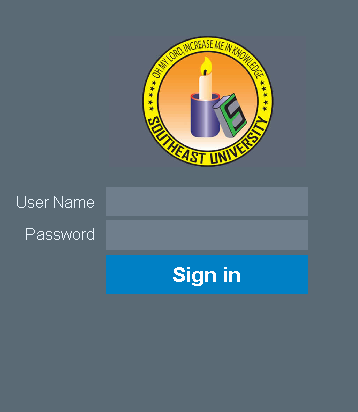
\includegraphics[width=.5\textwidth]{pic/login_page.png}
	\end{center}
	\caption{Log-in Page}
	\label{fig:login_page}
\end{figure}


Logging in is a process where an individual access into a secured computer system by entering authentic identification. Here, in this page a authentic user must enter valid username and password to access the main system to perform a task. After successful logging in Home page will be appeared. Which user when access to the system, it will be stored in the database for security purpose. A valid user of course can modify the password and modify his own profile of course.


In, Figure-\ref{fig:login_page} the log-in page has been showed from this project. The user-name and password must be more than or equivalent to 4 characters and should be valid to access the home page. 





\section{Home Form}

A home page  is the initial page of a software application. It is also sometimes called main page as well. In, Figure-\ref{fig:home_page} the Home page has been showed. Any user with authentic username and password can access this page. In this page a user can see all the roles that has been assigned to that user.In this page a menu bar will be showed up in the header area of the page. By using the menu bar the user can go to the specific pages and does the jobs according to the roles.

\clearpage



%\begin{landscape}
\begin{figure}[h]
		\begin{center}
			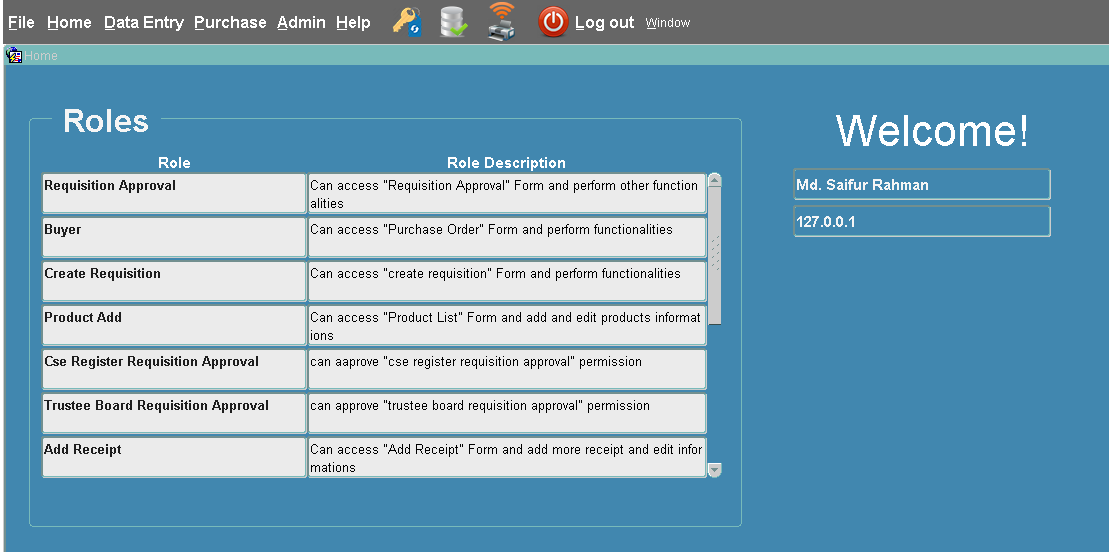
\includegraphics[width=1\textwidth]{pic/home_page.png}
		\end{center}
	\caption{Home Page}
	\label{fig:home_page}
\end{figure}
%\thispagestyle{empty} 
%\end{landscape}
%\clearpage

\ifx
\clearpage

\begin{figure}[h]
	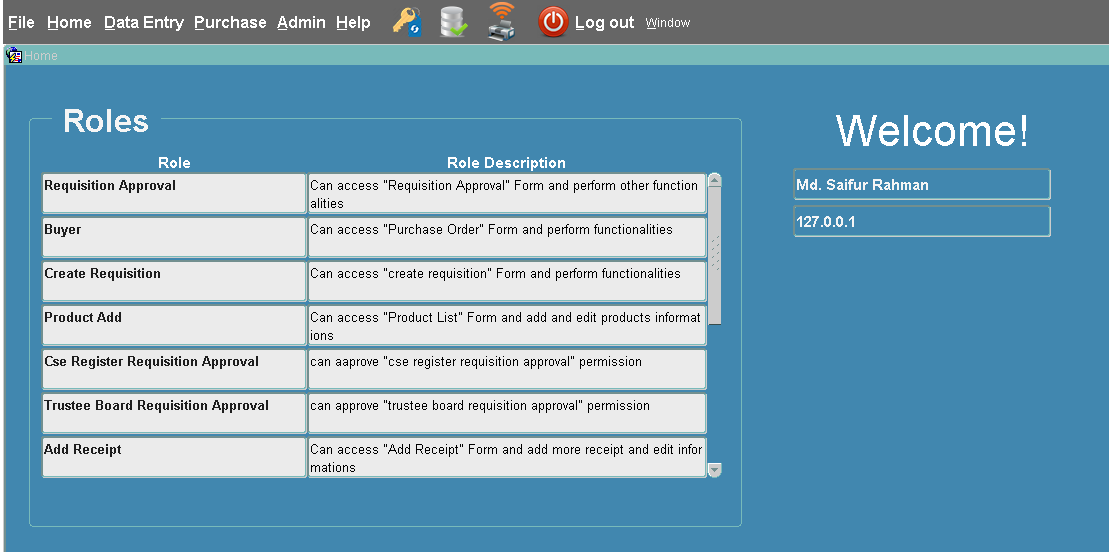
\includegraphics[width=1\textwidth]{pic/home_page.png}
	\caption{Home Page}
	\label{fig:home_page}
\end{figure}



\begin{landscape}
\subsection{Schema Diagram}
\begin{figure}[h]
	\begin{center}
		%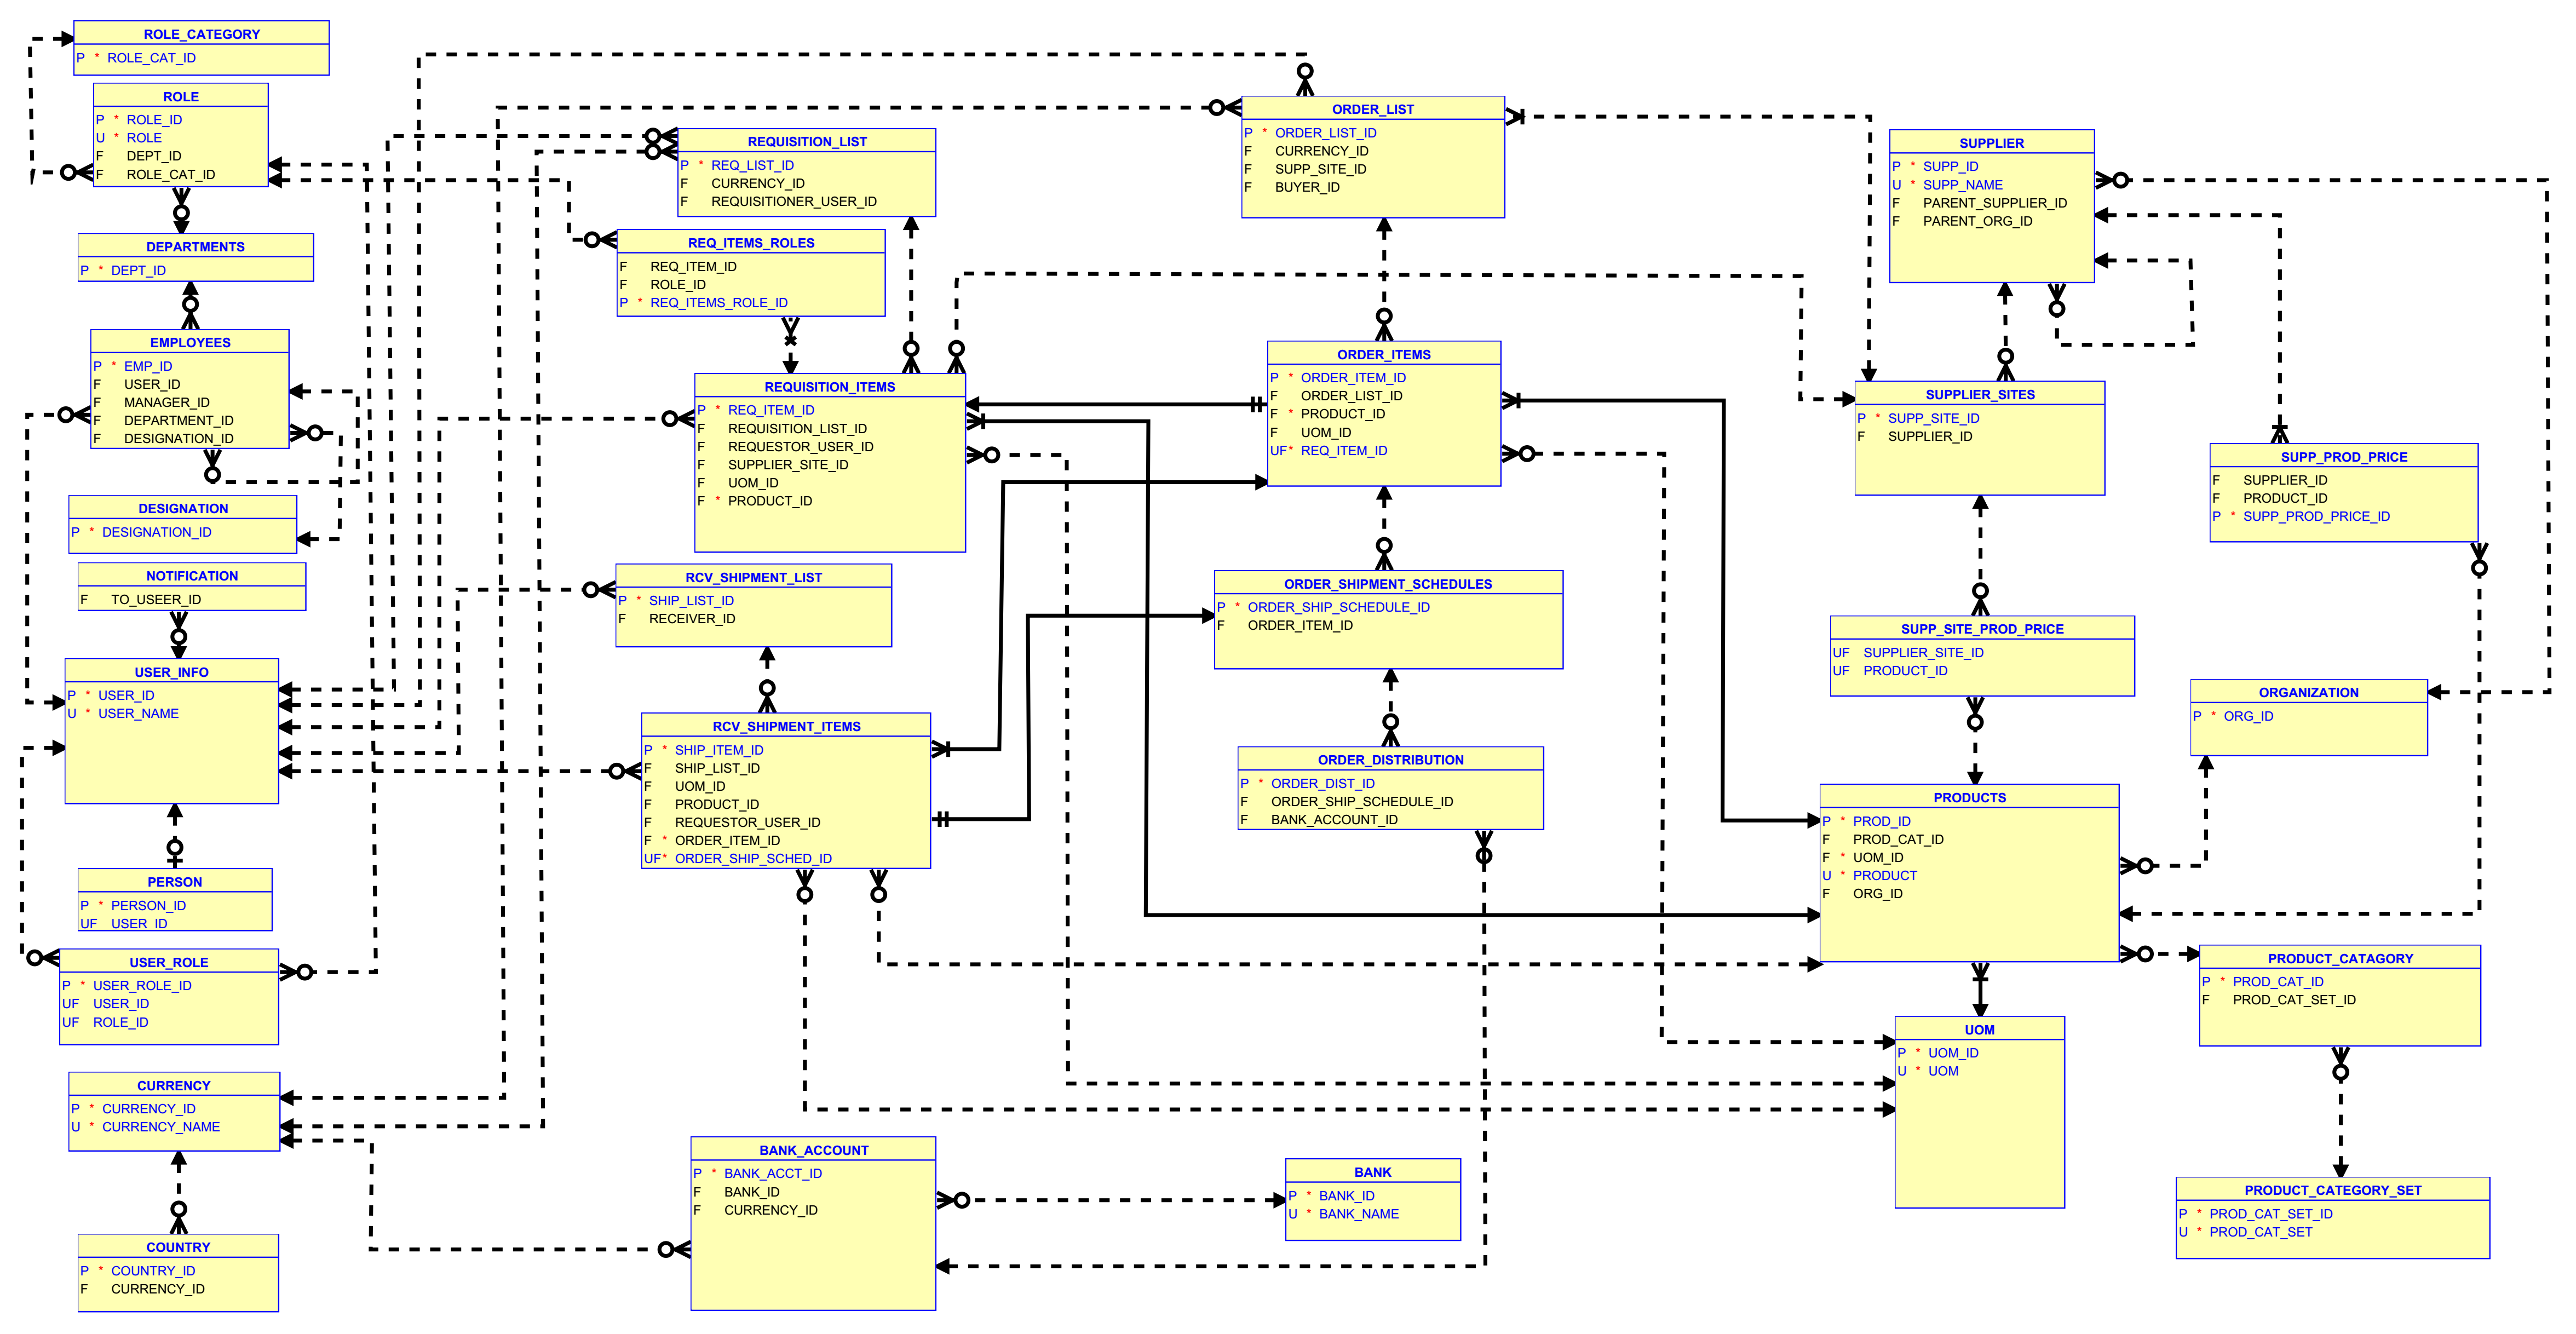
\includegraphics[width=0.95\textwidth, angle =90]{pic/schema/seupr_schema.png}
		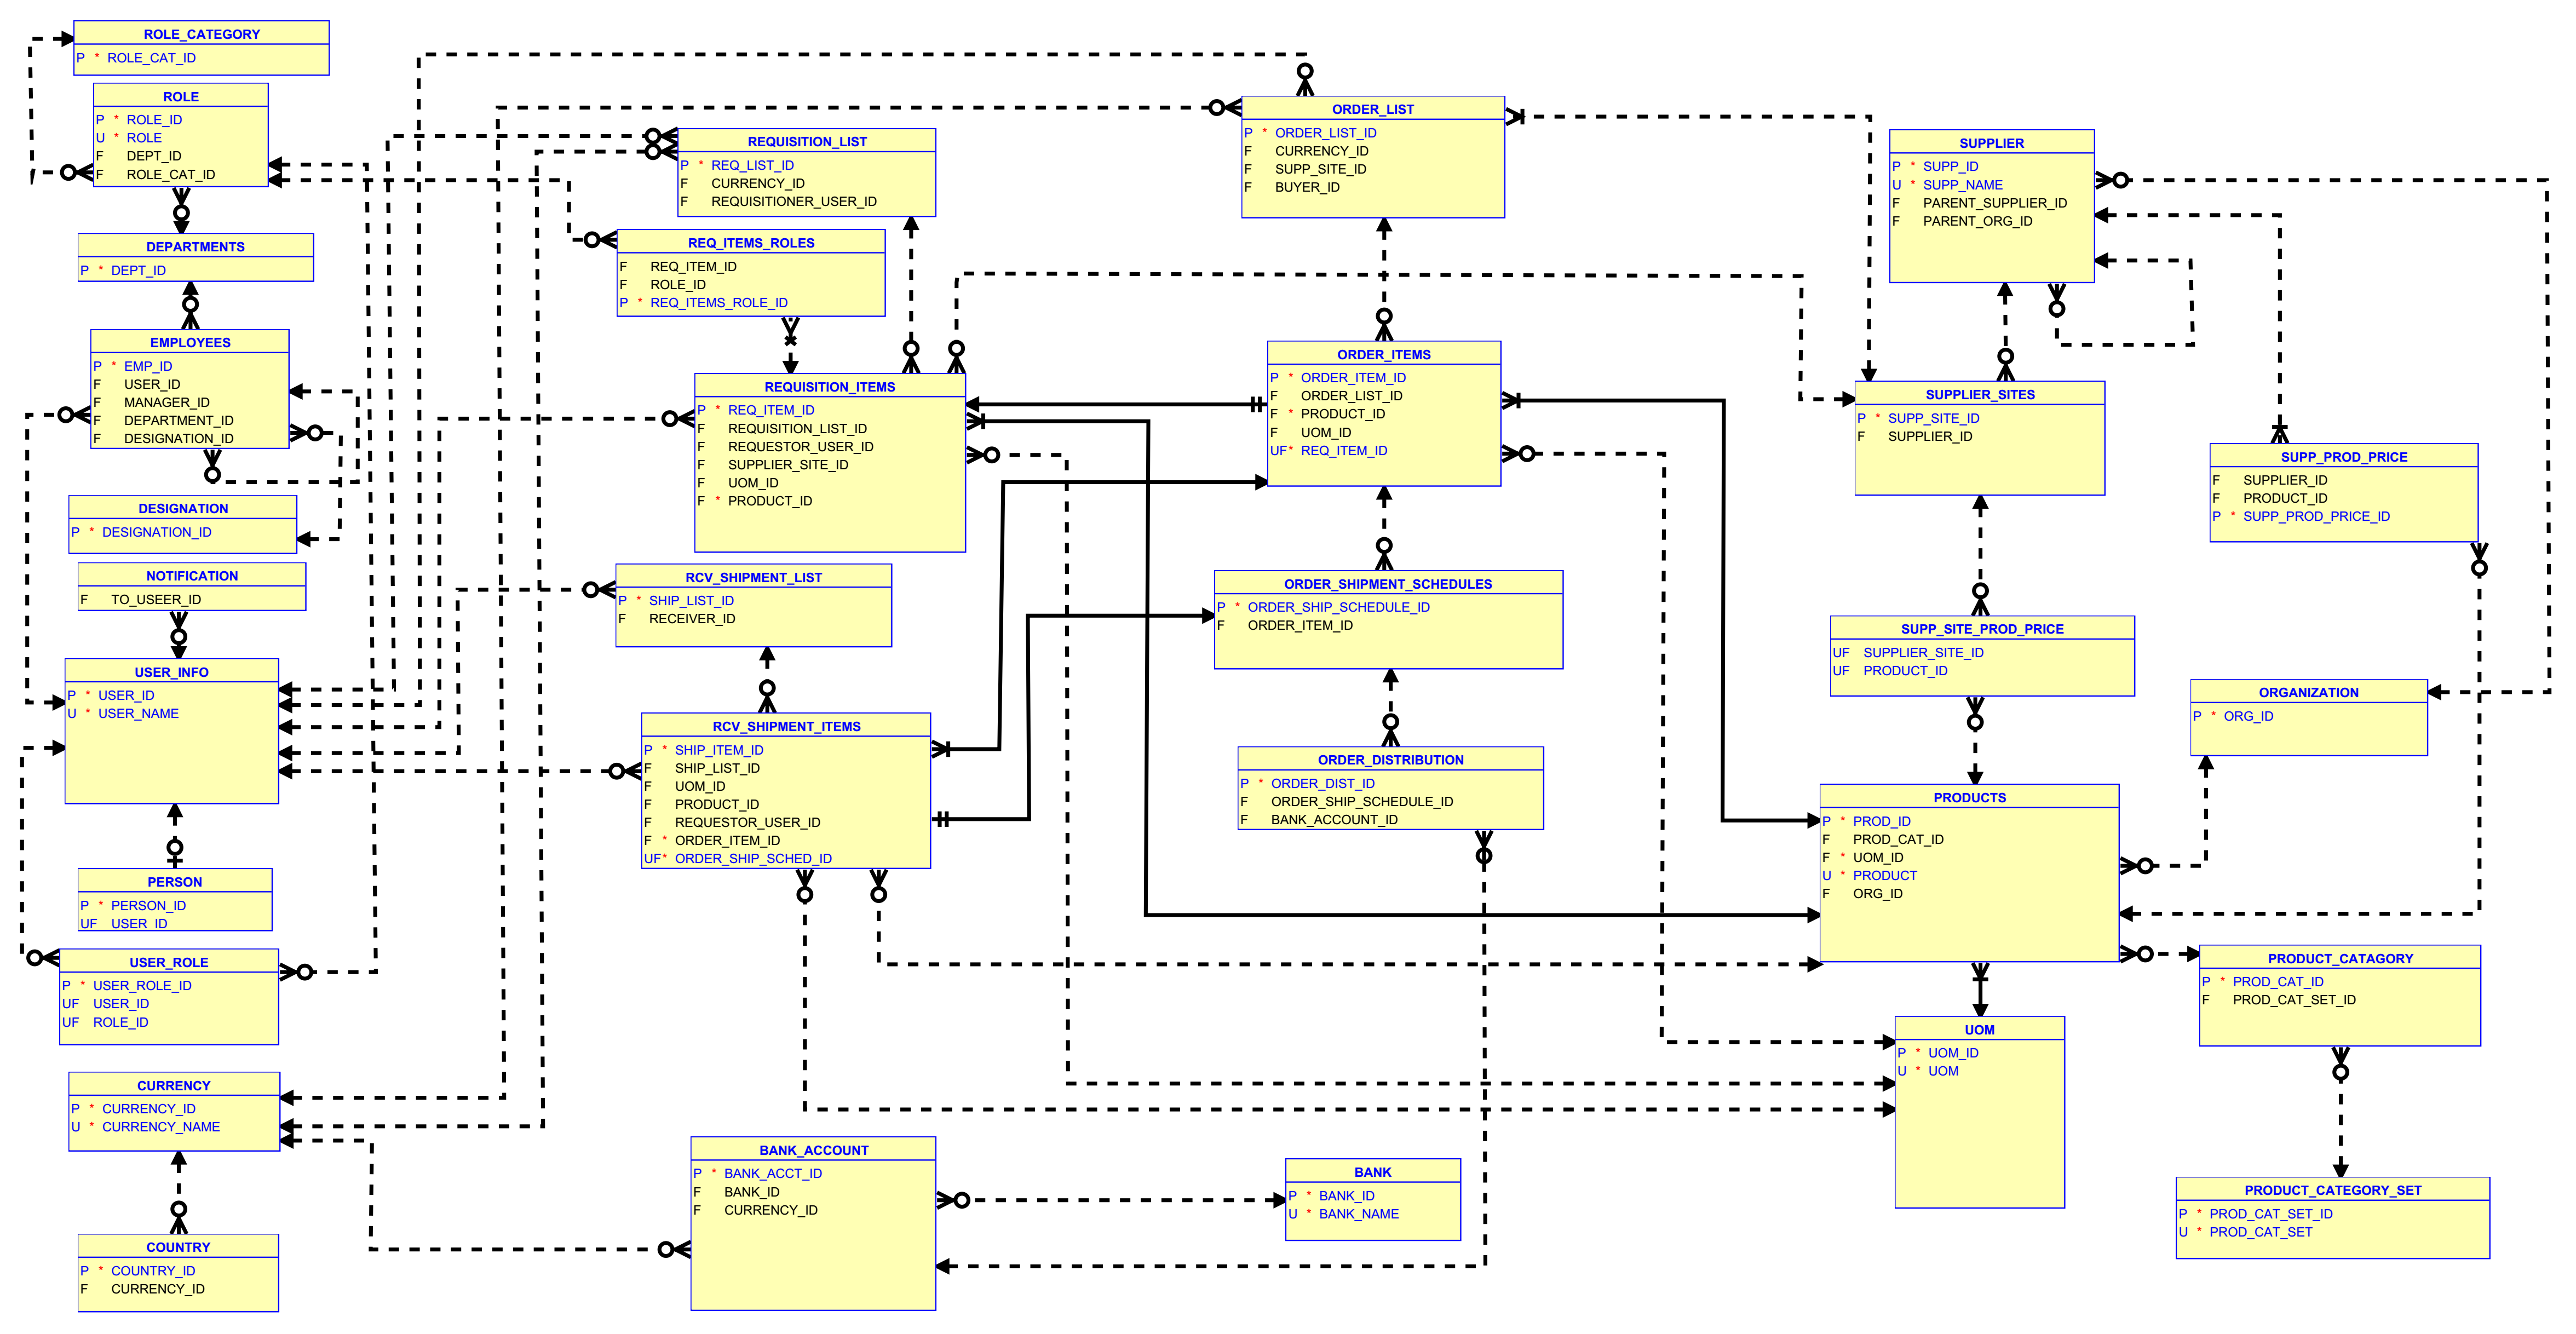
\includegraphics[width=1.3\textwidth]{pic/schema/seupr_schema.png}
	\end{center}
	\caption{Schema Diagram of SEU Purchase Requisition}
	\label{fig:context_level}
\end{figure}
\thispagestyle{empty} 
\end{landscape}
\clearpage
\fi

\section{Unit of measurement List Form}
\begin{figure}[h]
	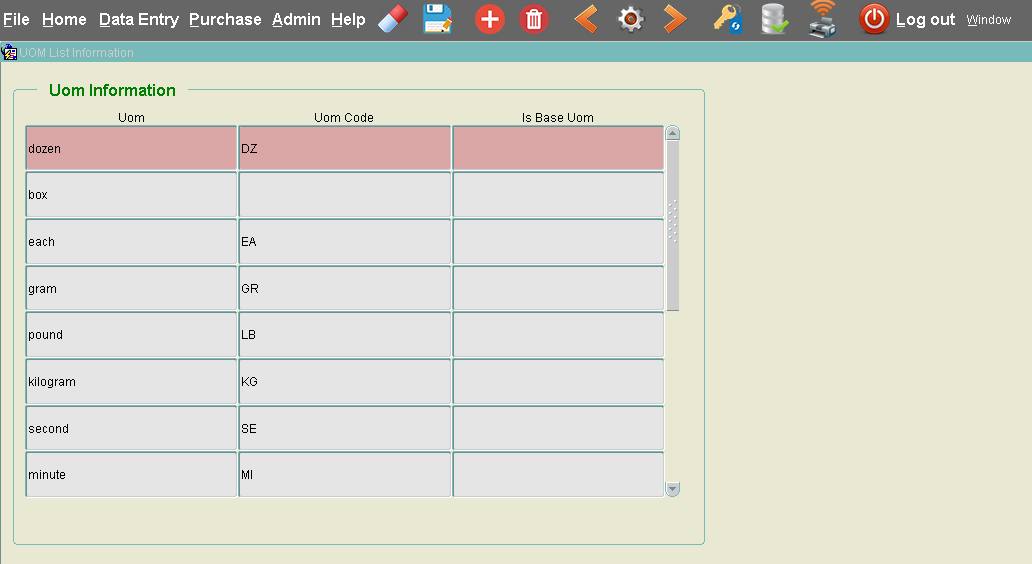
\includegraphics[width=1\textwidth]{pic/unit_list_page.PNG}
	\caption{Unit of Measurement List Page}
	\label{fig:unit_list_page}
\end{figure}
In, Figure-\ref{fig:unit_list_page} UOM list page has been showed.Here a user can add an UOM to the system if he/she has the sufficient privilege to do that. Suppose, an item is pen and it's unit of measures is \textbf{each} and UOM code is \textbf{EA}.   An UOM must be unique otherwise there an error will be prompted in that case. \\

\textbf{UOM (Unit of Measure):} along with a numeric value, to specify
the quantity of an item. For example, each is a unit of measure that is used to specify a singular number of units of an item. Units of measure are used to define the quantity of an item when defining, stocking, planning, ordering, transacting, shipping, receiving, and counting items.\\
%\clearpage



\section{Bank List Form}

\begin{figure}[h]
	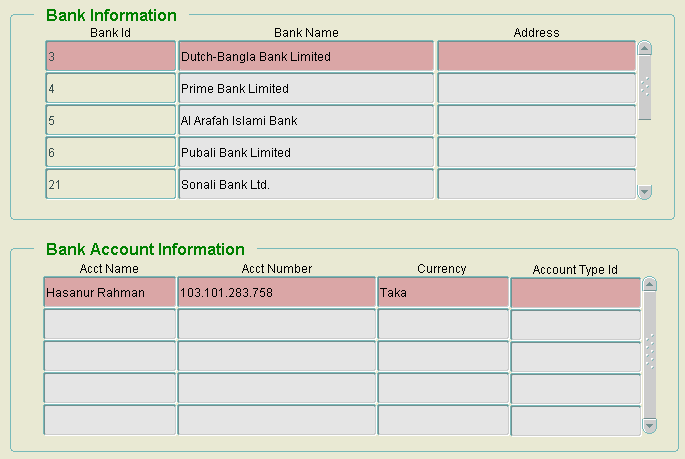
\includegraphics[width=1\textwidth]{pic/bank_list_page.PNG}
	\caption{Bank List Page}
	\label{fig:bank_list_page}
\end{figure}
In, Figure-\ref{fig:bank_list_page} the bank list page has been showed. Here, a user can add a bank name if he/she has the privilege.\\
\textbf{Bank id :} auto increment. User does not have to worry  Bank id.\\ 
\textbf{Bank name :} must be unique. \\
In Bank Account information block there can be multiple records and each record contains account name , account number, currency (in which currency the transactions will be occurred), account type. \\
\textbf{Acct Name:} Name of the bank account that this supplier or supplier site or employees of the organization uses. The list of values allow for only active supplier bank accounts. The user entry Bank Account name in Acct Name field supplier those supplier are active. \\
\textbf{Acct Number:} Bank account number of the bank account that this supplier or supplier site. User must entry supplier Account Number in Acct Number field.\\
\textbf{Currency :} have to use select currency if multiple currency is being used.




\section{Product List Form}
\begin{figure}[h]
	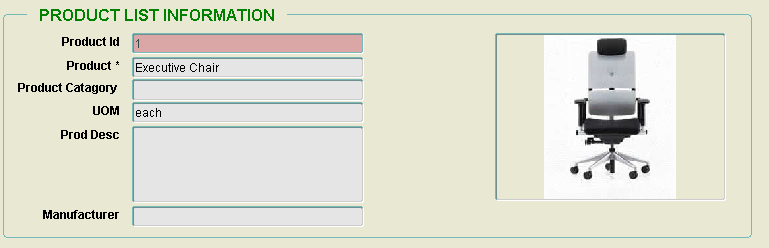
\includegraphics[width=1\textwidth]{pic/product_list_page.PNG}
	\caption{Product List Page}
	\label{fig:product_list_page}
\end{figure}
In, Figure-\ref{fig:product_list_page} the product list page has been showed. Here, a user can add a product information if the user has the sufficient privilege.\\ 
\textbf{product id :} is the auto generated number which is generated by the system.\\
\textbf{Product name : } must be unique. \\
\textbf{UOM :} (Unit of Measurement) can be selected from the LOV(List Of values). When user clicked the lov button then a list will be prompted with data then user can select one of them and it be set to the UOM field. \\
\textbf{product Description : } user can add description of that product.\\
 \textbf{picture :} select any picture with the format of .jpg, .png, .gif can be added to load in the database and then it will be retrieved automatically from the database when forms will be executed in the new-form-instance happened. \textbf{Caution: } Picture must be located in this 
 \ifx
 \begin{lstlisting}[
    basicstyle=\small  %or \small or \footnotesize etc.
]
``D:\SAIFURSOFT\SEUPR\images" location to load in the database.
\end{lstlisting} 
\fi


\section{Supplier List Form}


In, Figure-\ref{fig:supplier_list_page} a user can add a supplier to the system and manage the suppliers if the user has the sufficient role or privilege to do that. \\
In this form supplier id is auto generated by the system, user shouldn't worry about that. Supplier name field must be entered and it should be unique as well. In organization name field the organization name of the supplier can be added. Bank account number is to be selected using lov button. The bank account number will be retrieved from the list of bank account. URL is the website where the supplier broadcasting their products. Inactive date is from which date the supplier can't do any dealing with the organization. Tax registration number and tax payer id can be added here too.\\
In supplier site information block at least one supplier site record should be added. In each record supplier site address , supplier site phone, supplier site name and agent name should be added.\\
In supplier site product price block product name can be selected using lov and then UOM would be automatically filled by the system. User should be added a valid price there and also put comments. User can add multiple products here their specific price.
%\clearpage

%\begin{landscape}
\begin{figure}[h]
	\begin{center}
		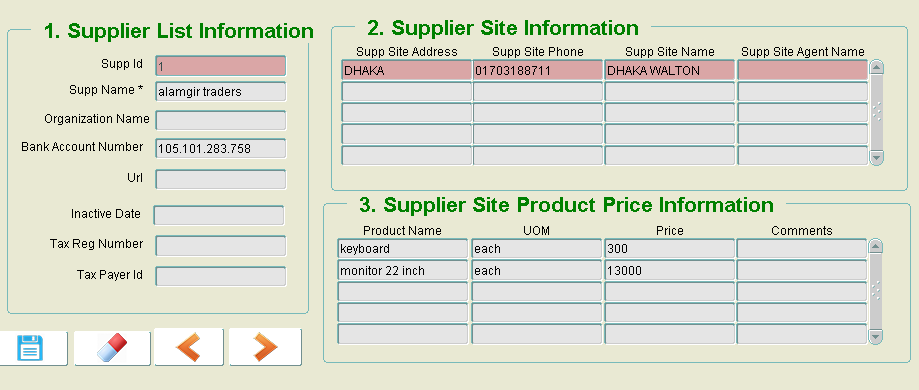
\includegraphics[width=1\textwidth]{pic/supplier_list_page.PNG}
	\end{center}
	\caption{Supplier List Page}
	\label{fig:supplier_list_page}
\end{figure}
%\thispagestyle{empty} 
%\end{landscape}
%\clearpage


\ifx

\begin{figure}[h]
	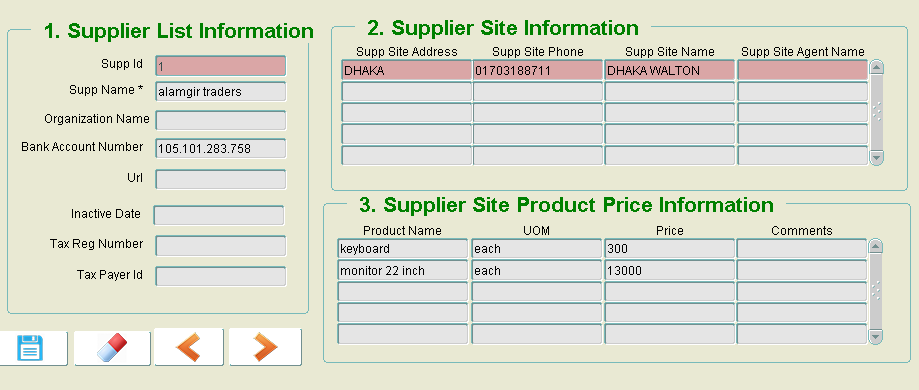
\includegraphics[width=1\textwidth]{pic/supplier_list_page.PNG}
	\caption{Supplier List Page}
	\label{fig:supplier_list_page}
\end{figure}
\clearpage

\begin{landscape}
\begin{figure}[h]
		\begin{center}
			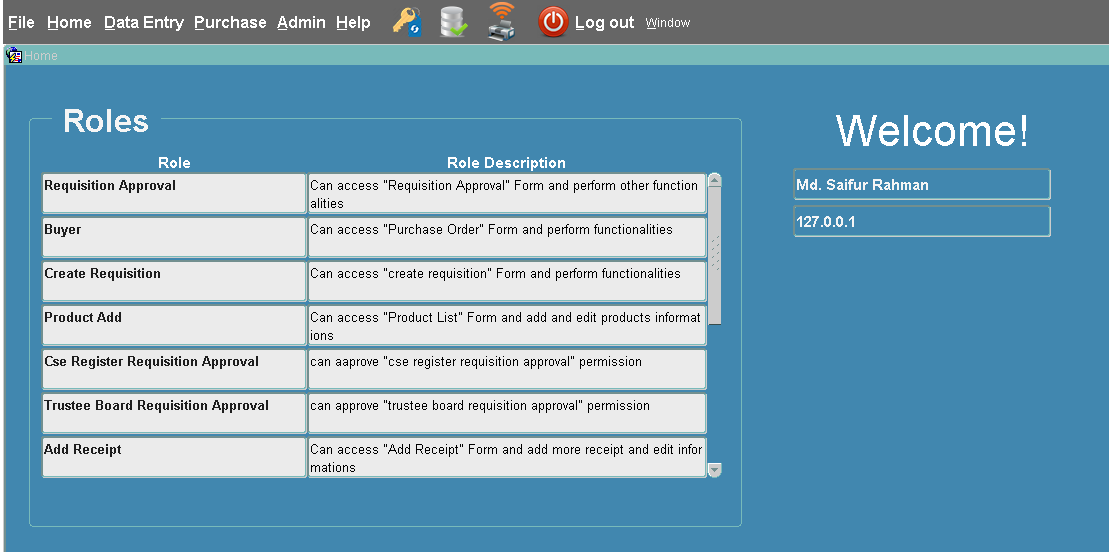
\includegraphics[width=1.5\textwidth]{pic/home_page.png}
		\end{center}
	\caption{Home Page}
	\label{fig:home_page}
\end{figure}
\thispagestyle{empty} 
\end{landscape}
\clearpage
\fi

\section{Requisition Entry Form}
During a Requisition lifecycle, many people can act on the requisition including Employees, Buyers or buyer-planners, Approvers, Suppliers, Purchasing staff or employees. Here a requisition generator creates a requisition who must be a registered user and an employee of SEU of course and must have "Create Requisition" privilege. An employee can create requisition list which can contain multiple requisition items. In the description section a requisition generator can tells if it's urgent or not. In which currency the transactions will be occurred the user can select it using lov that has been assigned to that field. Prepared by and last updated time field will be automatically filled by the system.\\

In each requisition items, there will be information about requisition item id,the requestor's demanded product name (selected by using LOV), the requestor name(selected by using LOV), price of the product, quantity of that product that is required (QTY), total amount(which is automatically calculated, total amount = QTY * price ), supplier site name, need by date, delivery locations and so on. Each item must need all level of approvals before generating purchase order against that requisition item.\\

Here, if the total amount for an item is less than or equal to 3000 then one approval is needed. If item total amount is greater than 3000 and less than or equal to 10,000 then it will need 2 approvals  and if item total amount is greater than 10,000 then it will need 3 approvals. In this way the new rules can be applied. This is an automatic system. One trigger is created to complete this task. The trigger's code is given below. The software developer must maintain the code when the rules will be changed.\\%codes
%\clearpage



\begin{table}

	\begin{tabular}{|l|}
	\hline
	\begin{lstlisting}[
	    basicstyle=\tiny, %or \small or \footnotesize etc.
	]
	CREATE OR REPLACE TRIGGER REQ_ITEM_ROLES_LOAD_TR
	AFTER UPDATE OF  QTY,PRICE ON REQUISITION_ITEMS  
	FOR EACH ROW
	DECLARE
	    TOTAL_AMUNT SEUPR.REQUISITION_ITEMS.PRICE%TYPE;
	BEGIN
	    TOTAL_AMUNT := NVL(:NEW.QTY, 0)*NVL(:NEW.PRICE, 0);

	    IF UPDATING AND (NVL(:OLD.QTY, 0) != NVL(:NEW.QTY, 0) OR NVL(:OLD.PRICE, 0) != NVL(:NEW.PRICE, 0)) THEN

	        IF(TOTAL_AMUNT>=10000) THEN
	            DELETE FROM REQ_ITEMS_ROLES WHERE REQ_ITEM_ID=:NEW.REQ_ITEM_ID ;
	            INSERT ALL
	                INTO REQ_ITEMS_ROLES (REQ_ITEM_ID, ROLE_ID) VALUES (:NEW.REQ_ITEM_ID,1)
	                INTO REQ_ITEMS_ROLES (REQ_ITEM_ID, ROLE_ID) VALUES (:NEW.REQ_ITEM_ID,2)
	                INTO REQ_ITEMS_ROLES (REQ_ITEM_ID, ROLE_ID) VALUES (:NEW.REQ_ITEM_ID,3)
	            SELECT * FROM dual;

	        ELSIF(TOTAL_AMUNT>=3000 AND TOTAL_AMUNT<10000) THEN
	           DELETE FROM REQ_ITEMS_ROLES WHERE REQ_ITEM_ID=:NEW.REQ_ITEM_ID ;

	            INSERT ALL
	                INTO REQ_ITEMS_ROLES (REQ_ITEM_ID, ROLE_ID) VALUES (:NEW.REQ_ITEM_ID,1)
	                INTO REQ_ITEMS_ROLES (REQ_ITEM_ID, ROLE_ID) VALUES (:NEW.REQ_ITEM_ID,2)
	            SELECT * FROM dual;

	        ELSIF(TOTAL_AMUNT<3000) THEN
	            DELETE FROM REQ_ITEMS_ROLES WHERE REQ_ITEM_ID=:NEW.REQ_ITEM_ID ;
	            INSERT ALL
	                INTO REQ_ITEMS_ROLES (REQ_ITEM_ID, ROLE_ID) VALUES (:NEW.REQ_ITEM_ID,1)
	            SELECT * FROM dual;
	        END IF;

	        COMMIT;
	    END IF;

	    EXCEPTION
	          WHEN OTHERS THEN
	            NULL;
	END;
	\end{lstlisting}\\
	\hline
	\end{tabular}
\end{table}


In Requisition Amount Distribution block there will be multiple records for each requisition items. Each record holds a bank account(suggesting an account to be charged) which is selected by using LOV, expenditure percent can't be more than 100\% then expenditure amount's field will be automatically filled by system calculation.\\

Requisition items roles block is only for view. A used can ad or modify any information here. This page is for requisition creator so that he/she can view which approver and when did or didn't approve the requisition item and for which reason with comments.
In, Figure-\ref{fig:req_list_page} Requisition Entry Form is being showed. Some key things to remember :

\renewcommand{\labelenumi}{\alph{enumi})}
\begin{enumerate}

		\item After inserting and saving items in the requisition items block, the items cannont be deleted
		\item Requisitioner has to wait to take it further steps till all the approvals for that item is being approved
		\item Only the user who created the requisition item can access his/her own created item
		\item If the requisition item once saved it cannot be changed by the creator
\end{enumerate}



\newgeometry{bottom=1cm,left=2cm, top=1cm, right=0cm}
\begin{landscape}

%\clearpage
\begin{figure}[h]
	\begin{center}
	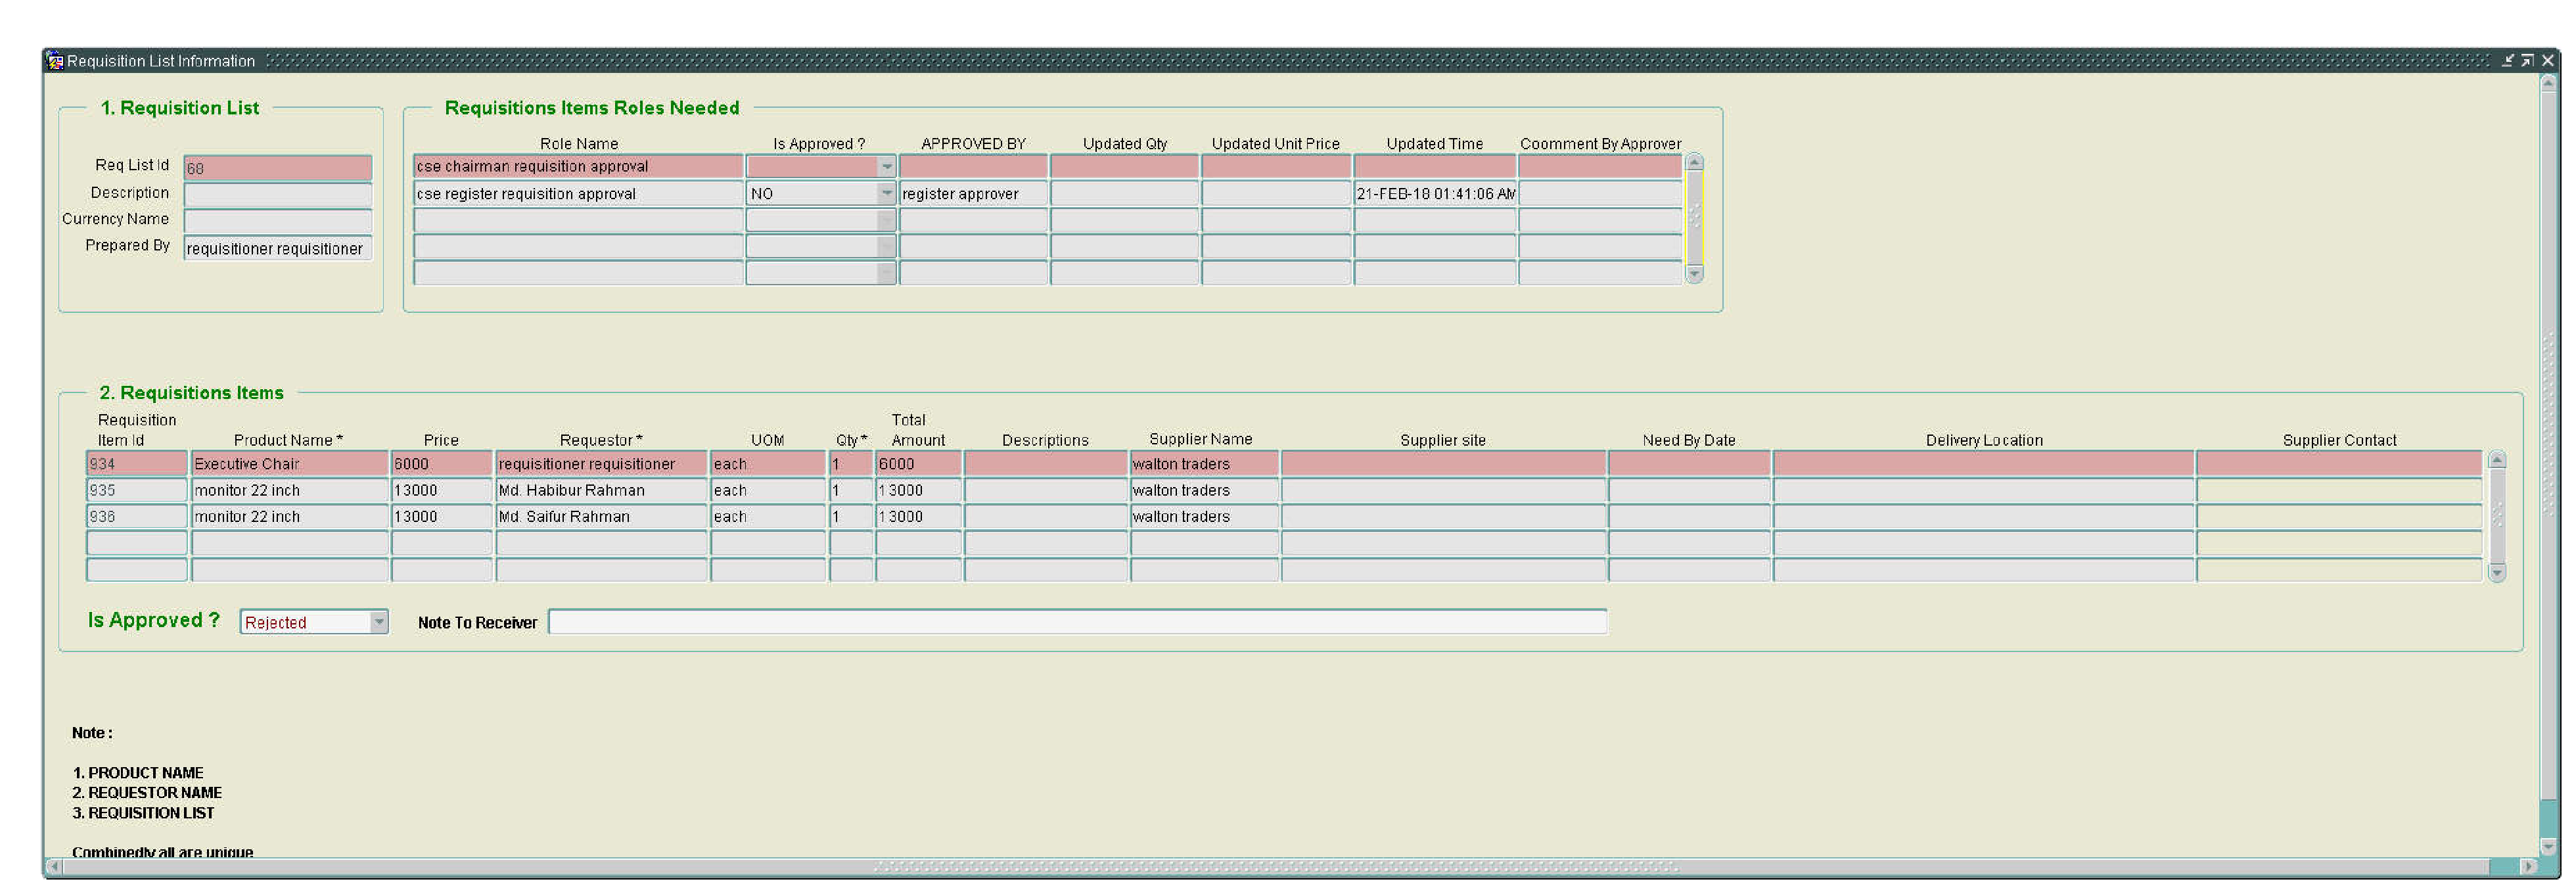
\includegraphics[width=1.35\textwidth]{pic/req_list_page.PNG}
	\end{center}
	\caption{Requisition List Page}
	\label{fig:req_list_page}
\end{figure}
\thispagestyle{empty} 
\end{landscape}
\clearpage







\begin{landscape}
\section{Requisition Approval List Form}
A user with the role of ``Requisition Approval" can access the form. Requisition items block is only for view. An approver can select one item from here to give approval. In requisition item roles needed block an approver ha to select yes or no in ``is approve?" field. Once all the approval is given as yes by all the approvers then the item will be approved and it connot be changed anymore.
Suppose, if a requisition item needs 3 approvals. If first approver gives approval then second approver can gain power to give approval. Again if second approver gives approvals then third approver can give approval. 
\begin{figure}[h]
	\begin{center}
		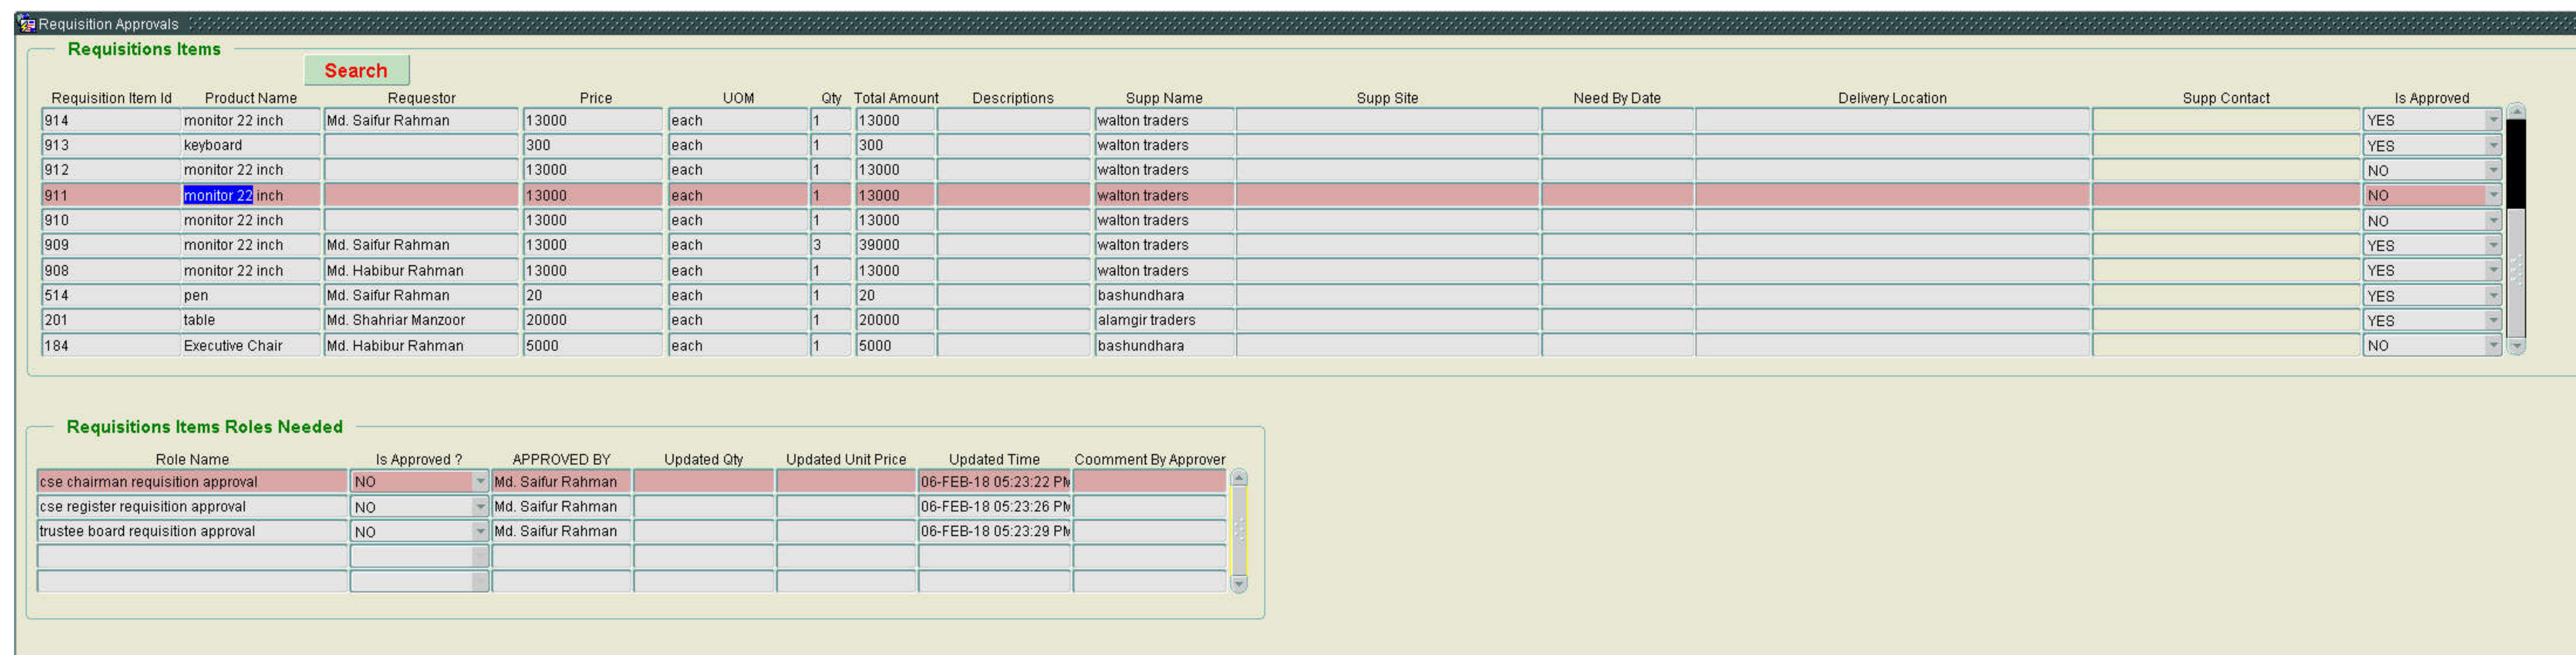
\includegraphics[width=1.35\textwidth]{pic/req_approval_list.PNG}
	\end{center}
	\caption{Requisition Approval List Page}
	\label{fig:req_approval_list}
\end{figure}
\thispagestyle{empty} 
\end{landscape}
\clearpage
\restoregeometry






\section{Purchase order Form}
To access purchase order form a user must need "Buyer" role. A buyer can create a order and in that order can contain multiple order items. In the Order Entry block the buyer has to fill order type. In this case, order type is standard purchase order. Buyer has to add currency name, supplier name, supplier site by using different lov. Buyer should also add Description and Bill to location in the specific fields. \\

In the order items block, buyer can add multiple order items. Each order items can contains order item id which is automatically generated by the system and buyer shouldn't worry about that. Each order item must be against a unique requisition item. It is strictly restricted by the system. Buyer don't have to worry about that matter. Requisition item id is selected by the buyer using ``Requisition item lov". Then Product name, UOM, price will be automatically filled by the system.\\

Each order item contains multiple shipment schedule if needed. Shipment schedules total qty, and charge amount will not be crossed cause of system automatic restriction. \\

Each shipment schedules contains multiple order distributions. Each distribution contains the bank account, expenditure percent and charge amount.
\clearpage


\newgeometry{bottom=1cm,left=2cm, top=1cm, right=0cm}

\begin{landscape}
\begin{figure}[h]
	\begin{center}
	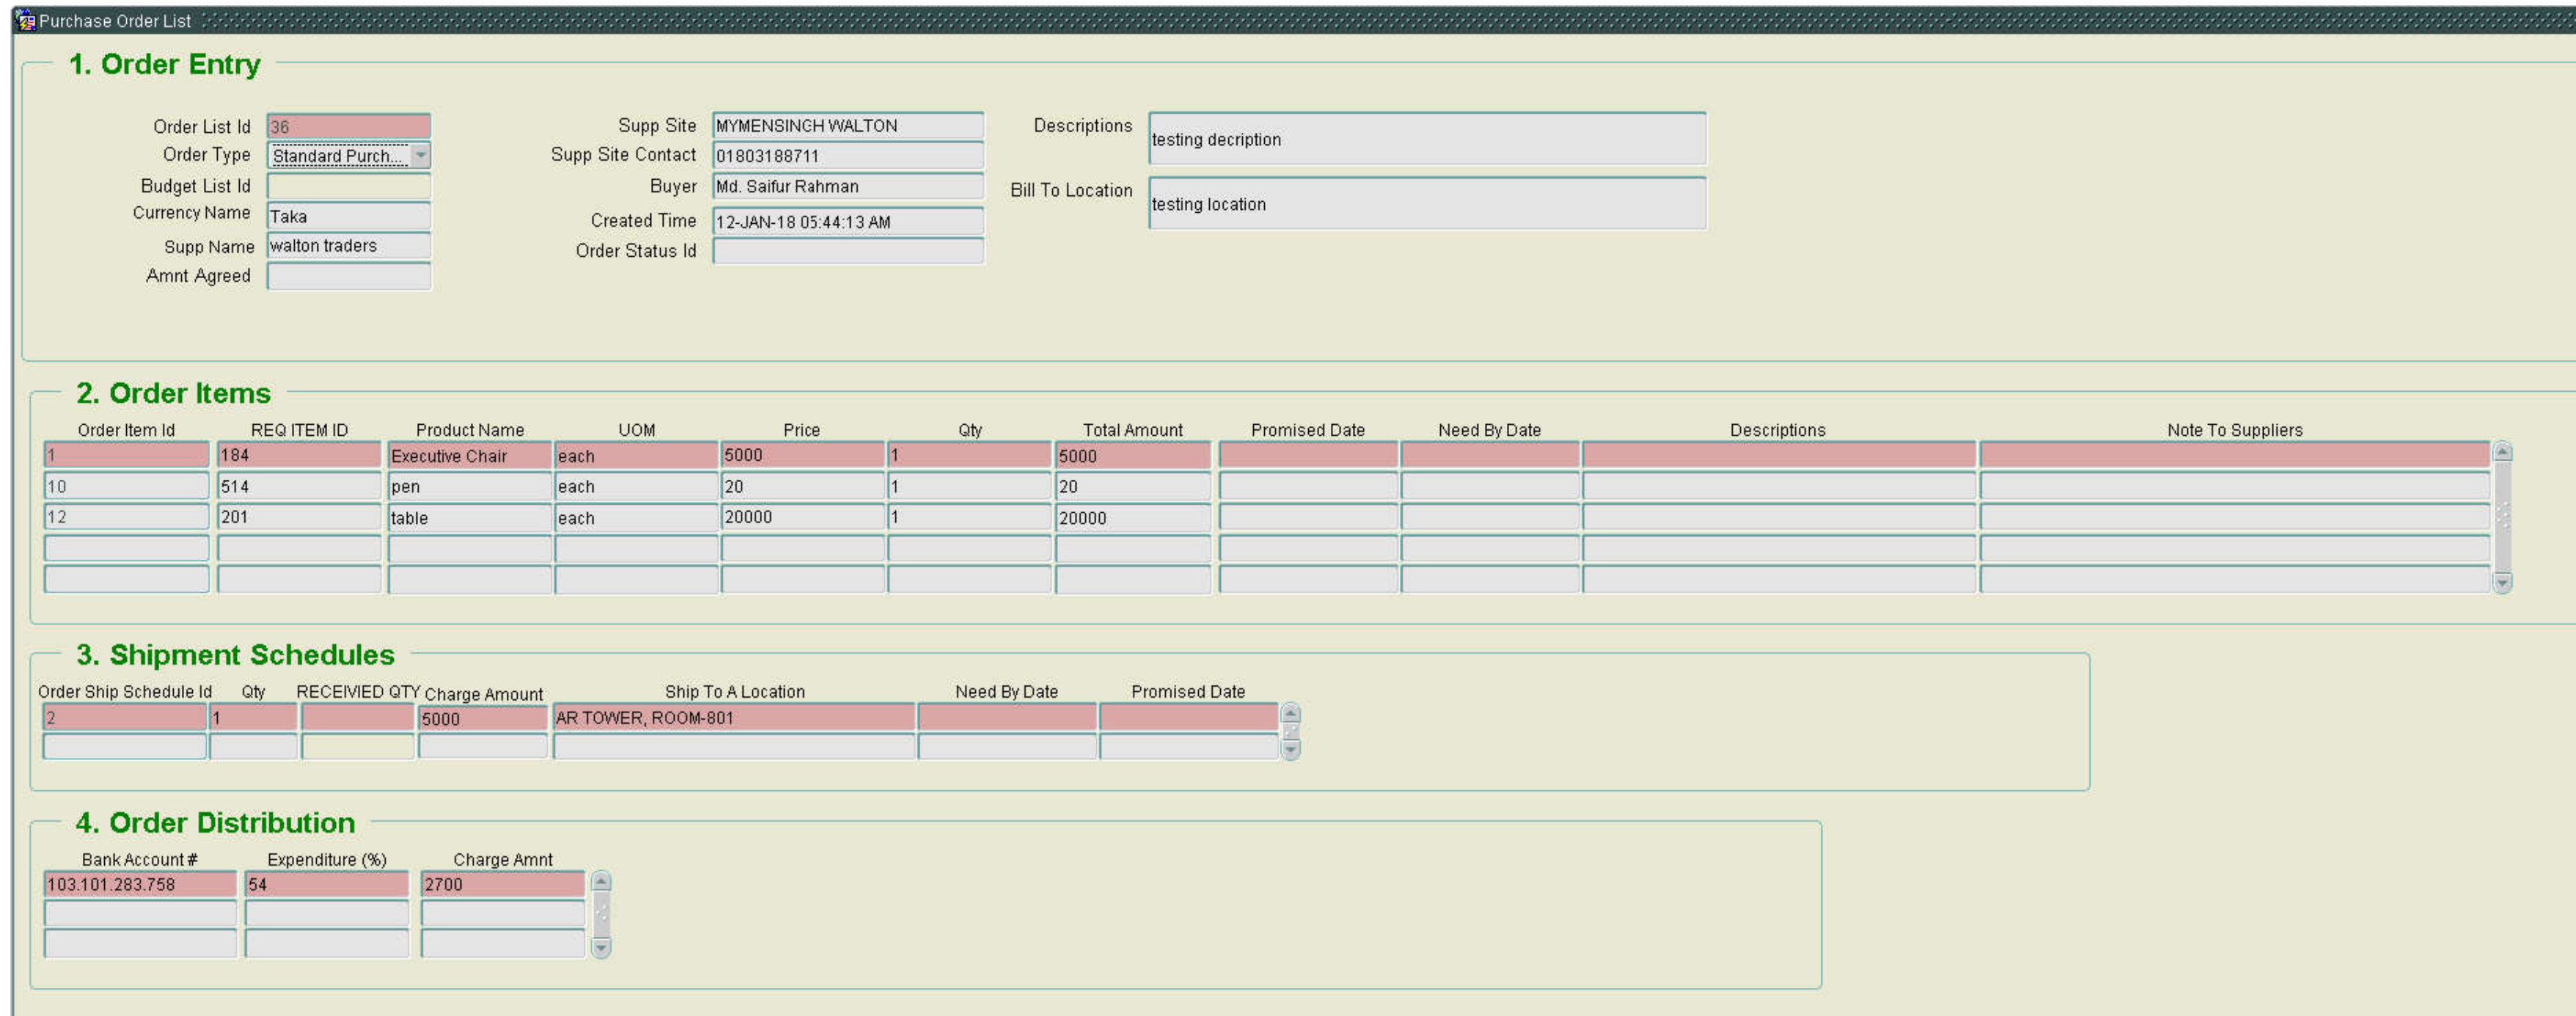
\includegraphics[width=1.35\textwidth]{pic/Pur_order_page.PNG}
	\end{center}
	\caption{Purchase order Page}
	\label{fig:Pur_order_page}
\end{figure}
\thispagestyle{empty} 
\end{landscape}
\clearpage





\begin{landscape}
\section{Receipt Form}
To access the Receipt form a user must have ``Add Receipt" Role. After accessing the receipt form a receiver all he has to do is write the name and select order shipment schedule id by using lov that has been set to that item and and write the received qty. Other than these three things a receiver doesn't have to do anything. It's very simple and all things are generated automatically by the system for more user friendly environment. Receipt date will be automatically set by system. UOM, requestor name, Expected qty and note to receiver will be automatically set. Commenting will be a good practice for future analysis and make the receipt form much more understandable.
%\clearpage
\begin{figure}[h]
	\begin{center}
	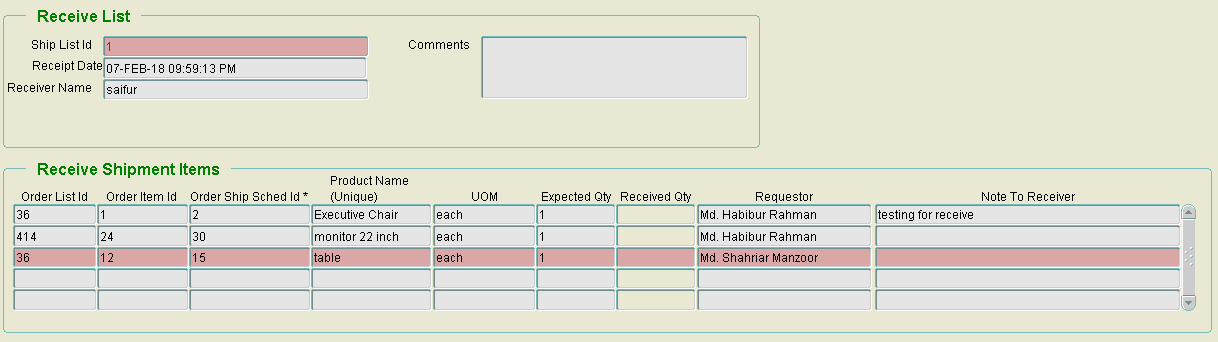
\includegraphics[width=1.35\textwidth]{pic/receipt_list_page.PNG}
	\end{center}
	\caption{Receipt Page}
	\label{fig:receipt_list_page}
\end{figure}
\thispagestyle{empty} 
\end{landscape}
\clearpage



\restoregeometry





%\begin{landscape}
\section{User Information Form}
To access the User Information form a user must have ``Add User" Role. Normally system administrator does have that kind of permissions. Administrator add user with roles to access the software application and do some specific functions. in this form the user must have to fill the user name and password field and first name and last name field to save the page.\\
Administrator should add some roles to the new user to access specific forms. The roles are uniquely added to the new user or already existed users too in the user roles block section. One thing to be remembered that role name must be unique for each user. %Though it is restricted by system. User doesn't have to worry about that.
\begin{figure}[h]
	\begin{center}
		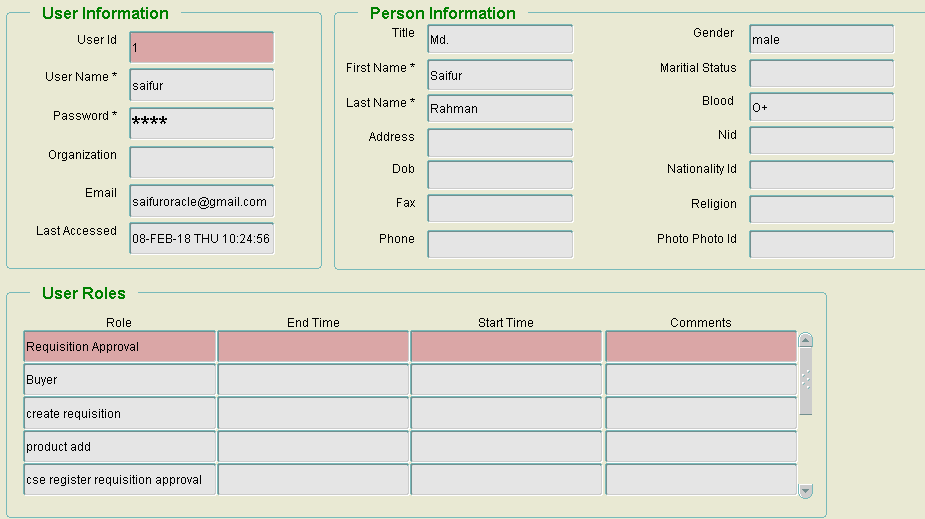
\includegraphics[width=1\textwidth]{pic/user_info_page.PNG}
	\end{center}
	\caption{User Information Page}
	\label{fig:user_info_page}
\end{figure}
%In, Figure-\ref{fig:user_info_page} User Information Form page has been showed.

%\thispagestyle{empty} 
%\end{landscape}
\clearpage




%\begin{landscape}
\section{Roles Form}
To access the Roles form a user must have ``Add Role" Role. In this page normally for administrator user. The user add new unique roles for system privacy maintenance for user access controlling.\\
In Role information block role id is auto generated by system. Role is unique and user has to add new role by following organization policy. Role description is described as what is the purpose of that role.\\
In user role information block a user has to add user name by using lov and person name field will be automatically filled by the system. Start time means starting date from when the role is applied for that user and end time means when the role is terminated for that user. 
\begin{figure}[h]
	\begin{center}
	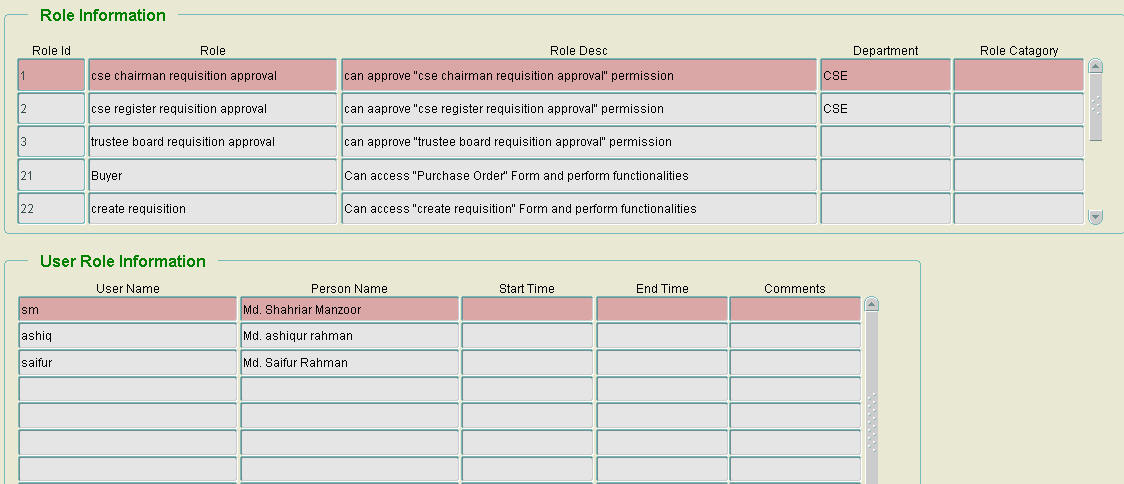
\includegraphics[width=1\textwidth]{pic/Roles_page.PNG}
	\end{center}
	\caption{Roles Page}
	\label{fig:Roles_page}
\end{figure}
%In, Figure-\ref{fig:Roles_page} Roles Form page has been showed.
%\thispagestyle{empty} 
%\end{landscape}
\clearpage



\section{Profile Form}
This page is for only user. Any user can access his/her own profile and edit information. User can add phone, blood group, address, Date of birth(DOB), NID, Marital status, select gender and so on. User also can change user name and email. Note, user role information is only for view for the user.\\
\textbf{Title : } These can be titles prefixing a person's name. Like Mr, Mrs, Miss, Ms, Sir, Dr.\\
\textbf{First name \& Last Name: }First name is the person first part of the name. Last name is the person last part of the name. For example, Habibur Rahman, here Habibur is the first name and Rahman is the last name.\\
\textbf{Address :} is the location where the user is currently living.\\
\textbf{Dob :} is date of birth of the user.\\
\textbf{Phone :} is the contact number of the user\\
\textbf{Blood Group :} Human blood groups.  like, O+,O-, A+, A- and so on.\\
\textbf{NID :} National Identity (NID) Card. Its use as a voter's identity card. If the user is more than 18 years old then he must have an NID.\\
\textbf{Gender :} male or female or other can be selected\\
\textbf{Religion :} Islam, Hinduism, Christianity , etc.\\
\textbf{Username :} is the name to access the software.\\
\textbf{Email :} xxx@gamil.com, xxx@yahoo.com, etc\\
\textbf{Organization :} where the user works\\
\clearpage


%\newgeometry{bottom=1cm,left=2cm, top=1cm, right=0cm}
%\begin{landscape}
\begin{figure}[h]
	\begin{center}
	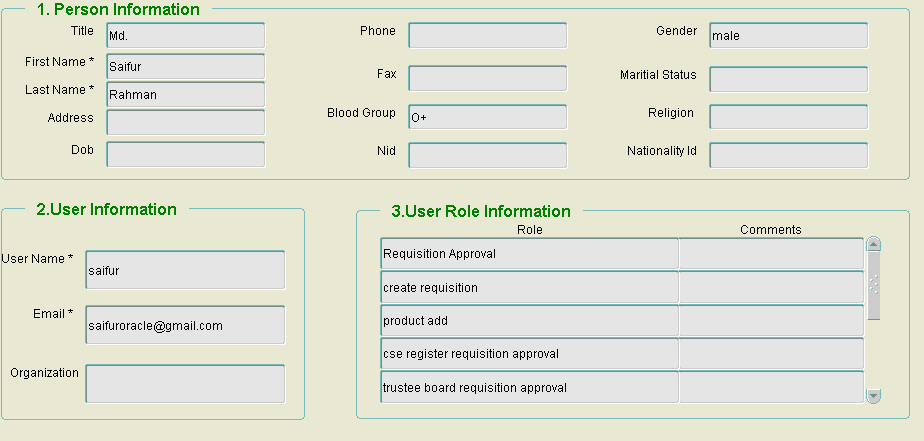
\includegraphics[width=1.1\textwidth]{pic/profile.PNG}
	\end{center}
	\caption{Profile Page}
	\label{fig:profile}
\end{figure}
%\thispagestyle{empty} 
%\end{landscape}
%\restoregeometry



\section{Notification Form}
This page is for user to get instant message of the actions performed by other users. Suppose in requisition approval list form, if an item has all the approval yes then creator of that requisition item get a notification message with item id, time, which user performed the action, what approval is given and note. This notification system is created for users for better usage of the software and make this software very much user friendly. User can also delete all the notifications by clicking the Delete all button.
\begin{figure}[h]
	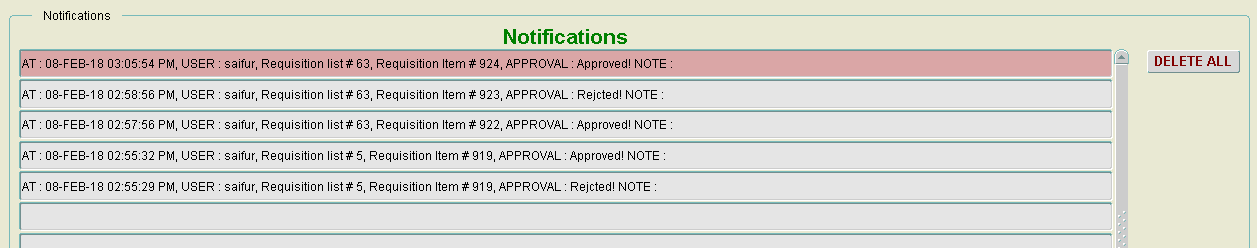
\includegraphics[width=1\textwidth]{pic/notification.PNG}
	\caption{Notification Page}
	\label{fig:notification}
\end{figure}
%In, Figure-\ref{fig:notification} Notification Form page has been showed.


\section{Change Password Form}
In this page any user can access. The user can change the password by giving valid old password. The new password and re-type password must match to save the password. \\
\textbf{Note:} New password length must be greater than or equivalent to 4 character.\\
\begin{figure}[h]
	\begin{center}
	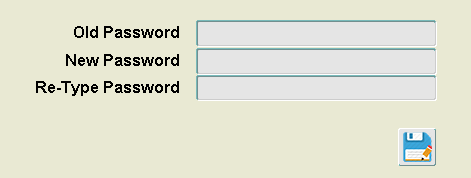
\includegraphics[width=0.6\textwidth]{pic/change_pass.PNG}
	\end{center}
	\caption{Change Password Page}
	\label{fig:change_pass}
\end{figure}
%In, Figure-\ref{fig:change_pass} Change Password Form page has been showed.


%clearing the left portion of the page

\clearpage

%Chapter 3 Overview of the project  End HERE----------
%Chapter 3 Overview of the project  End HERE----------









%Chapter 4 Implementation and Result  Start HERE----------
%Chapter 4 Implementation and Result  Start HERE----------
%\chapter{Implementation and Result}
\ifx
\section{Graphical User Interface}
Graphical user interface is type of user interact that allow to interact with electronic devices with images rather than text commands. This is the software's \textbf{login page}. A user must log-in before accessing the main software to do his/her works by typing the user-name and password accurately. 
\fi






%clearing the left portion of the page
%\clearpage

%Chapter 4 Implementation and Result  end HERE----------
%Chapter 4 Implementation and Result  Staendrt HERE----------















\ifx
\chapter{Results \& Evaluation}
\setcounter{page}{1}
\thispagestyle{empty}    %ADD IMMEDIATELY BEFORE EVERY CHAPTER

\section{Results}
This thesis is an applied research. Here a purchase requisition management system has been implemented for SEU authority.
%design error, weak areas 
\fi







\chapter{Limitations and Conclusion}
%\chapter{Conclusion and Further Work}
\setcounter{page}{1}
\thispagestyle{empty}    %ADD IMMEDIATELY BEFORE EVERY CHAPTER
\section*{Conclusion}
% important and final part, summarized,provide future lead for improvements, main points, show your idea why it matter to them, 
%so waht? why it is important? what is the meaning of your paper?
%Give something you readier to thinkk about after finishing the story
This software projects is based on purchase requisition management system using Oracle Forms 10g. In here user creates requisition list which contains requisition item and each of them needs approvals. After being approved, a notification will be sent to the creator of that requisition item by the system automatically and the requisition item can be added as an order item in an order list by a buyer and purchase the item from suppler site. Then items are supplied by vendor and it is received by a receiver and the process ends. The user can made the purchase process in a single platform and don't have to waste time unnecessarily when the system is online. It needs more functionality like tender, auction process, market analyzing and other business processes to make it fully compatible to the SEU purchase requisition management system.


\section*{Limitations and Boundaries}
Limited time, lack of resources and lack of industry level experiences are the main reasons for the limitations and boundaries of this project. Right now this software isn't accessible to everyone. It will be if there is a unique real IP and network configurations can be done. This software will be well designed and well be described to make it more user reliable, robust and user friendly in future implementations. This project requires jdk 6 version which isn't quite appreciable for current time application users but jdk 8 will be used in future implementations. 


\section*{Recommendations on Future Improvement}
\ifx
There is always room for improvements. In this software there are so many other functionalities to add. In future, this project can be implemented in Oracle E-Business Suite or Oracle Application Express or  Oracle Forms 12c to make this project more reliable and more robust and more user friendly and will be added some more business functions. In addition, the software can also be improved in terms of the calculations it can perform, and the rates of flexibility used in calculations per user. If any problem will be generated in the future the developers will try best to solve the issues. 
\fi
There is always room for improvements. In this software there are so many other functionalities to add.

%http://smallbusiness.chron.com/checklist-purchasingprocess-audit-45378.html

\renewcommand{\labelenumi}{\alph{enumi})}
\begin{enumerate}
	\item This project can be implemented in Oracle E-Business Suite or Oracle Application Express or  Oracle Forms 12c to make this project more reliable and more robust
	\item Tender and Auction system can be added to maintain tender process. That part can describe the cost of the contract, submit the best prices, prices are compared to other vendors prices, cooperating about the quality of the goods or services during a specific periods.
	\item Supplier Comparisons in terms of product's quality, price etc. Analyzing the Actual Costs, communicating different providers, Measuring Supply Performances. 
	\item Messaging System : For example, requisitioner wants to reminds the approver by a message to ensure requisition item approval.
	\item Audit : To control risks, prevent fraud, ensure maximum savings and maintain regulatory requirements and maintain periodic audits to avoid unwanted risks. 
	\item Vendor Validation : Analyzing, if the vendor's plays an integral role in the organization, if they follow the guidelines, policies and continue to meet company criteria as SEU required.
	\item Quality Assessment : By continuous checking the reports of the quality once the goods or services are received. Checking inventory reports, patterns of poor or damaged products may lead to review of the vendor's suitability for the organization.
	%\item Inquiries : Analyzing information from a purchase order, 
	
\end{enumerate}

\section*{Contribution}

The purchase requisition management system is a new project in Southeast University. In the past no one worked on this subject. It may be a good solution to help the procurement process undoubtedly. And this is a nonprofit software application.




%\chapter*{References}
%\setcounter{page}{1}
%\thispagestyle{empty}    %ADD IMMEDIATELY BEFORE EVERY CHAPTER
%Reference PAGE start HERE----------
%Reference PAGE start HERE----------


%Format of Citations and References
%Creating a Reference Page in APA
%https://www.youtube.com/watch?v=s_jZy3kJd6E
%How to write reference in project report or research paper?
%http://nob.cs.ucdavis.edu/classes/ecs015-2007-02/paper/citations.html
%https://www.youtube.com/watch?v=10eg_GB_A9E             Using APA style for references and citations


%biblatex - How to go back to body after visiting a reference?------------------



%format:
%    Structure: Last, F. M. (Year Published) Book. City, State: Publisher.
%    Examples: James, H. (1937). The ambassadors. New York, NY: Scribner.
%    Examples: Rowling, J.K. (2001). Harry Potter and the socerer's stone. London: Bloomsburg Children's.
%    Format: Last name, F. M. (Year Published) Book. Retrieved from URL.
%    Examples: James, H. ( 2009). ...
%    Format: Last, F. M. (Year Published). Book. ...
%    Examples: Morem, S. ( 2005).
%    https://www.youtube.com/watch?v=gGtkh_-9OC0&list=PLJte6w3fUL6tnN8wb_hndiZViJzZNpcDI (apa styles)
\pagestyle{empty}
\setcounter{page}{0}
\renewcommand\bibname{References} % Removing thebibliography title
\begin{thebibliography}{1}
\addcontentsline{toc}{chapter}{\refname} %make bibliography as reference chapter 
  \bibitem{purchase_module_book}  \hyperref[sec:purchase_module_book_1]{Mitchell, V. \& Simpson, D.F. (2007). R12 Oracle purchasing fundamentals.} 
  \bibitem{sql_book} \hyperref[sec:sql_book_1]{Clement, S. \& Pottle, B. \& Singh, P. (2010). Oracle Database: SQL Fundamentals I.}
  \bibitem{sql_book2} \hyperref[sec:sql_book_1]{Koratamaddi, C. \& Pottle, B. \& Srivastava, T. (2010). Oracle Database: SQL Fundamentals II.}
  
  \bibitem{plsql_book} \hyperref[sec:plsql_book_1]{Pottle, B. (2009). Oracle Database 11g: PL/SQL Fundamentals.}
  \bibitem{plsql_book2} \hyperref[sec:plsql_book_1]{Serhal, L.K. (2009). Oracle Database 11g: Develop PL/SQL Program Units.}
  
  \bibitem{form_builder_book}  \hyperref[sec:form_builder_book_1]{Gamer, P. (2006). Oracle Forms Developer 10g: Build Internet Applications.}
  
  \bibitem{norman} \textit{Oracle Purchasing User's Guide}. (2018, January 10). Retrieved  from  {\url{https://docs.oracle.com/cd/E18727_01/doc.121/e13410/toc.htm}}
  
  \bibitem{norman} Greenwood, S. (August 3, 2015). The future of Oracle Forms. Retrieved  from  {\url{http://www.explorer.uk.com/the-future-of-oracle-forms/}}
  
  \bibitem{feature_forms} \hyperref[sec:feature_forms_1]{ \textit{The future of Oracle Forms}. (2018, February 10). Retrieved  from  {\url{https://www.toadworld.com/platforms/oracle/w/wiki/11125.the-future-of-oracle-forms}} }
  
  
  %\bibitem{notes} John W. Dower {\em Readings compiled for History
  %21.479.}  1991.

  %\bibitem{impj}  The Japan Reader {\em Imperial Japan 1800-1945} 1973:
  %Random House, N.Y.

  %\bibitem{norman} E. H. Norman {\em Japan's emergence as a modern
  %state} 1940: International Secretariat, Institute of Pacific Relations.

  %\bibitem{fo} Bob Tadashi Wakabayashi {\em Anti-Foreignism and Western
  %Learning in Early-Modern Japan} 1986: Harvard University Press.

  \end{thebibliography}
  

 \thispagestyle{empty}    %ADD IMMEDIATELY BEFORE EVERY CHAPTER
\clearpage

%Reference PAGE ends HERE----------
%Reference PAGE ends HERE----------






\end{document}
